\documentclass{fast-nuces-bs}
%\documentclass{article}

\usepackage{blindtext}
\usepackage{mathptmx}% Times Roman font
\usepackage[T1]{fontenc}
\usepackage{lipsum} 
\usepackage{sectsty}
\usepackage{tikz-uml}
\usepackage{titlesec}
\usepackage{longtable,booktabs,array,graphicx,xcolor,tabularx,multirow,enumitem,float,caption,listings,url}
\usetikzlibrary{arrows.meta,positioning,shapes.geometric,fit,calc,backgrounds,decorations.pathreplacing}
\graphicspath{{./ThesisFigs/}{../screenshots/}{./figures/}}
\setlist{itemsep=2pt,topsep=4pt}
\setlength{\tabcolsep}{3pt}
\sloppy\setlength{\emergencystretch}{3em}
\renewcommand{\arraystretch}{1.12}
\setlength{\parindent}{0pt}\setlength{\parskip}{5pt}
\lstset{basicstyle=\ttfamily\footnotesize,breaklines=true,frame=single,columns=fullflexible}
\tikzset{
  box/.style={draw,rounded corners=2pt,align=center,font=\footnotesize,minimum height=0.75cm,inner sep=4pt,fill=white},
  ext/.style={draw,rounded corners=2pt,align=center,font=\footnotesize,minimum height=0.75cm,inner sep=4pt,fill=gray!18},
  grp/.style={draw,dashed,rounded corners=4pt,inner sep=7pt},
  arr/.style={-{Stealth[length=2mm]}},
  darr/.style={dashed,-{Stealth[length=2mm]}},
  lab/.style={font=\scriptsize,fill=white,inner sep=1pt},
}
% Items the team must confirm before submission are highlighted so they cannot be missed.
\makeatletter\g@addto@macro\UrlBreaks{\do\_\do\-\do\:}\makeatother
\newcommand{\code}[1]{\texttt{\detokenize{#1}}}
\newcommand{\pth}[1]{{\urlstyle{tt}\path{#1}}}
\usepackage{soul}
\newcommand{\confirm}[1]{{\sethlcolor{yellow}\bfseries\hl{[CONFIRM: #1]}}}

% Information about the Thesis 
% -----------------------------------------------------------------------------
% (All are compulsory, do not delete any line other than author Information)
% For e.g., usually there are 3 students in a group, so leave authorone, 
% authortwo, and authorthree, and delete authorfour.
%%%%%%%%%%%%%%%%%%%%%%%%%%%%%%%%%%%%%%%%%%%%%%%%%%%%%%%%%%%%%%%%%%%%%%%%%%%%%%%
\department{FAST School of Computing}
\faculty{Computer Science}
\degreeyear{2026}
\degreemonth{October}
\degreename{Computer Science}
\campuscity{Islamabad}
\authorone{Shahmeer Atif}{23I-0711}
\authortwo{Muhammad Umar}{23I-0782}
\authorthree{Muhammad Usman Al Haq}{23I-0585}
\supervisor{Syed Muhammad Saad Salman}
\sessionduration{ 2023--2027}
\deanname{Dr. Dean Computing}
\directorname{Dr. Director of the Campus}
\hodname{Dr. Head of Computer Science Department}
\fypcoordinatorname{Name of FYP Coordinator}
\title{Halite: AI-Powered Maintenance Diagnostics and Asset Intelligence Platform}
%%%%%%%%%%%%%%%%%%%%%%%%%%%%%%%%%%%%%%%%%%%%%%%%%%%%%%%%%%%%%%%%%%%%%%%%%%%%%%%

%%%%%%%%%%%%%%%%%%%%%%%%%%%%%%%%%%%%%%%%%%%%%%%%%%%%%%%%%%%%%%%%%%%%%%%%%%%%%%
% Former document starts below this
\def\projecttitle{Halite: AI-Powered Maintenance Diagnostics and Asset Intelligence Platform}
\def\studentone{Shahmeer Atif (23I-0711)}
\def\studenttwo{Muhammad Umar (23I-0782)}
\def\studentthree{Muhammad Usman Al Haq (23I-0585)}

\begin{document}

%\begin{acknowledgements}
%	Your acknowledgments here
%\end{acknowledgements}

%\begin{abstract}
%Briefly state the (1) research problem, (2) methodology, (3) key results, and (4) conclusion. Generally, abstracts are between 150 and 200 words–roughly 10-15 sentences.
%\end{abstract}

\cleardoublepage
\pagenumbering{roman}
\chapter*{Students' Submission}
\addcontentsline{toc}{chapter}{Students' Submission}
We certify that this report is submitted as the FYP-1 mid-report for the project titled \textit{\projecttitle}.
\vspace{1cm}
\begin{tabular}{p{0.58\textwidth}p{0.38\textwidth}}
Student 1: \studentone & Signature: \rule{0.25\textwidth}{0.4pt}\\[1cm]
Student 2: \studenttwo & Signature: \rule{0.25\textwidth}{0.4pt}\\[1cm]
Student 3: \studentthree & Signature: \rule{0.25\textwidth}{0.4pt}
\end{tabular}

\chapter*{Anti-Plagiarism Statement}
\addcontentsline{toc}{chapter}{Anti-Plagiarism Statement}
The students certify that this report is their own work and that all sources used in preparing the report have been appropriately acknowledged and referenced.

\chapter*{Authors' Declaration}
\addcontentsline{toc}{chapter}{Authors' Declaration}
We declare that the work documented in this report represents the work completed by the project team up to the FYP-1 mid-report stage. Contributions, tools, external components, and relevant sources are disclosed where applicable.

In particular, AI coding assistants (Claude Code, OpenAI Codex and Cursor) were used during development and during the preparation of this report. They are disclosed in Section~\ref{sec:tools} together with the checks the team applied to their output. The team is responsible for, and able to explain, every change and every statement in this report.

\chapter*{Abstract}
\addcontentsline{toc}{chapter}{Abstract}
Maintenance teams keep years of service reports whose diagnostic value is lost because the records are free text, scattered, and sometimes corrected by a later report that a keyword search never connects to the original. Halite is a maintenance diagnostics and asset-intelligence platform that turns such records into an evidence-linked knowledge graph. The research gap it addresses is the combination of graph-constrained retrieval with explicit record validity: a diagnostic answer should say not only which past records look similar, but which of them were later corrected.

This mid-report documents the first iteration, a working vertical slice on real data. It loads 2,079 public FAA Service Difficulty Reports for 118 aircraft into Neo4j, shows each aircraft's dated history, ranks investigative checks with a deterministic, documented heuristic, validates every cited record identifier against the graph, classifies pairs of records as conflicting or superseding, and routes uncertain cases to a human review queue. A React interface exposes these paths, and a GitHub Actions pipeline runs the tests and deploys a shared staging backend.

Validation so far consists of 194 backend and 171 frontend automated tests passing in continuous integration, and a bounded live run on one aircraft in which the conflict engine found all three FAA-recorded corrections for that aircraft. We do not claim diagnostic accuracy: the ranking is a heuristic aid, semantic retrieval is not yet built, and most of the corpus has not been analysed. FYP-2 continues with hybrid retrieval, evaluation against baselines, role-based access, and the training and analytics modules.

\chapter*{Acknowledgments}
\addcontentsline{toc}{chapter}{Acknowledgments}
The project team thanks its supervisor, Syed Muhammad Saad Salman, for his supervision and guidance throughout the project, and the faculty of the FAST School of Computing. We thank the Federal Aviation Administration for publishing the Service Difficulty Report data openly, and the maintainers of the open-source software on which Halite is built.

\chapter*{Executive Summary}
\addcontentsline{toc}{chapter}{Executive Summary}

\textbf{Problem.} A technician investigating a recurring fault needs to know which symptoms occurred before, which components were examined, which repairs failed, and which earlier reports a later report has since corrected. Ordinary search returns similar documents but cannot say whether they still stand. Halite addresses this over public FAA Service Difficulty Reports (SDR): 2,079 records covering 118 aircraft.

\textbf{What exists at FYP-1 Mid.} The proposal planned nine modules. This iteration delivers a vertical slice through four of them, on real data, with the same commit passing automated tests in continuous integration:
\begin{itemize}
\item \textbf{Asset intelligence:} a fleet list and a dated history for each aircraft, with every record's original FAA identifier.
\item \textbf{Knowledge graph:} \code{Asset} and \code{ServiceRecord} nodes in Neo4j joined by \code{ABOUT}, \code{PRECEDED_BY} and \code{SUPERSEDES} relationships, shown one aircraft at a time.
\item \textbf{Diagnostics:} a symptom-based investigation that retrieves bounded graph context, ranks inspection checks with a deterministic heuristic, and verifies every cited record identifier against the graph. A model phrases the answer (and, in the multi-turn Copilot, extracts facts from the technician's message); it never decides the ranking. If no live model is available the system reports that instead of inventing a diagnosis.
\item \textbf{Conflict intelligence:} classification of record pairs (supersedes, partially supersedes, contradicts, scope-disjoint, no conflict), a confidence score, and a human review queue with accept and reject actions.
\end{itemize}
A CSV upload path, a React user interface, and a continuous-integration and staging-deployment pipeline complete the slice.

\textbf{Research findings.} Retrieval bounded by the graph (same aircraft, at least one matching signal, no records from the future) keeps conflict analysis tractable: on the largest aircraft (153 records) exhaustive pairing would need 11,628 comparisons. The FAA's own ``supplemental report'' wording gave us 141 correction pairs as ground truth without hand labelling.

\textbf{Validation status.} 200 backend and 171 frontend tests pass in GitHub Actions on the evaluated commit. A live re-validation of the diagnosis path on 18 October found a defect that the tests had missed (a function that returned nothing, so every fresh one-shot diagnosis failed); it was fixed, and diagnosis then succeeded on both the local stack and shared staging. A bounded live run on one aircraft (800NN, 13 records) found all three FAA-recorded corrections for it. An older offline evaluation of the conflict engine (350 evaluated pairs, threshold 0.50) reported precision 0.903, recall 0.660 and F1 0.762; it is historical evidence for conflict detection only and is not a measure of diagnostic accuracy.

\textbf{Honest limits and risks.} The diagnostic ranking is a lexical heuristic, not a trained model, and its scores are not probabilities. Semantic retrieval, authentication and organisations, the training module and analytics are not built. On the shared staging system every record is still unanalysed, because a full analysis run needs several days of model quota. Most of the code was merged in the last days before this report (Section~\ref{sec:timeline}), so each member's section states what they can demonstrate and explain.

\textbf{Remaining work.} FYP-1 Final adds hybrid retrieval, role-based access and session history; FYP-2 adds training, analytics, evaluation against baselines and production hardening (Chapter~\ref{ch:remaining}).

% The class prints the contents and the lists of figures and tables with the title page.
\chapter*{List of Abbreviations}
\addcontentsline{toc}{chapter}{List of Abbreviations}
\begin{tabular}{ll}
API & Application Programming Interface\\
ATA / JASC & Aviation maintenance chapter and component coding schemes used in SDR records\\
CI/CD & Continuous Integration / Continuous Delivery\\
CRUD & Create, Read, Update, Delete\\
FAA & Federal Aviation Administration\\
FR & Functional Requirement\\
FYP & Final Year Project\\
GenAI & Generative Artificial Intelligence\\
LLM & Large Language Model\\
NFR & Non-Functional Requirement\\
RAG & Retrieval-Augmented Generation\\
SDR & Service Difficulty Report (FAA)\\
SRS & Software Requirements Specification\\
UC & Use Case\\
UI / UX & User Interface / User Experience\\
UUID & Universally Unique Identifier\\
\end{tabular}


\cleardoublepage
\pagenumbering{arabic}
\chapter{Introduction and Project Vision}\label{ch:intro}

\section{Project Overview}
Halite is a maintenance diagnostics and asset-intelligence platform. It organises historical service records around the aircraft they describe, links each record to the record before it and to any later record that corrects it, and uses that structure to answer a technician's question: \emph{given this aircraft and this symptom, what has been seen before, what was examined, and what should be checked next?} Every answer names the records it rests on, and the system states plainly when it cannot answer.

Halite is decision support. It does not approve repairs, certify airworthiness, or replace licensed inspectors.

\section{Problem Statement}
Given an identified asset, a natural-language symptom, a corpus of historical service reports, and the possibility that some reports have been superseded or contradicted by later ones, design a system that retrieves relevant evidence, ranks investigative possibilities, and explains its recommendations without treating unsupported model output as fact. The system must preserve provenance, identify conflicting historical claims, and allow a human to intervene.

\section{Problem Context and Motivation}
Maintenance organisations accumulate service reports, inspection findings and corrective actions over the life of each asset. These records are free text, inconsistent in vocabulary, and sometimes wrong in hindsight. A retrieved report may describe a repair that did not work, or a finding that a later report corrected. In the FAA data we use, reporters sometimes file a ``supplemental report'' that names the earlier record it replaces, and the replacement may name a different component from the original. A search tool that returns the original as if it still stood misleads the technician; the correction is itself diagnostic evidence.

This is therefore not only a document-search problem. It is a problem of reasoning over evidence that changes over time, which is what motivates a graph that records order and correction explicitly, rather than a flat index of text.

\section{Project Vision}
To turn fragmented maintenance records into an accessible, explainable diagnostic knowledge system that helps maintenance teams investigate failures, understand earlier interventions, and learn from historical cases.

\section{Project Objectives}
The proposal lists thirteen objectives. Table~\ref{tab:objectives} states each one's status at this mid-report, with the measurable check we apply.

\begin{longtable}{p{0.04\textwidth}p{0.36\textwidth}p{0.14\textwidth}p{0.36\textwidth}}
\caption{Project objectives and their status at FYP-1 Mid}\label{tab:objectives}\\
\toprule
\textbf{\#} & \textbf{Objective} & \textbf{Status} & \textbf{Measurable check} \\ \midrule \endfirsthead
\toprule \textbf{\#} & \textbf{Objective} & \textbf{Status} & \textbf{Measurable check} \\ \midrule \endhead
1 & Structured maintenance knowledge graph & Done (Mid scope) & 2,079 records and 118 aircraft in Neo4j; relationships \code{ABOUT}, \code{PRECEDED_BY}, \code{SUPERSEDES} \\
2 & Record ingestion and normalisation & Partial & CSV ingest with explicit skip counts and duplicate safety; no free-text extraction \\
3 & Asset-aware historical retrieval & Done & Retrieval bounded to the aircraft history plus a capped fleet scan (Section~\ref{sec:alg-rank}) \\
4 & Semantic retrieval & Not started & Planned for FYP-1 Final; not claimed \\
5 & Evidence-aware diagnostic ranking & Done (heuristic) & Deterministic, documented weights; scores are not probabilities \\
6 & Interactive conversational investigation & Done (basic) & Multi-turn Copilot with carried case state \\
7 & Detect superseded and contradictory findings & Done & Five-label classifier with confidence and routing \\
8 & Human review for uncertain decisions & Done & Review queue with accept and reject; notes stored \\
9 & Educational diagnostic scenarios & Not started & Training module is FYP-2 \\
10 & Recurring-fault and fleet analytics & Not started & FYP-2 \\
11 & Secure multi-user SaaS application & Not started & No authentication yet \\
12 & Evaluation against controlled baselines & Partial & Historical conflict evaluation exists; diagnostic baselines not yet run \\
13 & Deployment with automated testing and CI/CD & Done & GitHub Actions on pushes to \code{main} and three named branches and on every pull request; CI-gated staging deploy \\
\bottomrule
\end{longtable}

\section{Project Scope}
\subsection{Included at FYP-1 Mid}
The iteration is a \emph{vertical slice}: one working path from real data to a cited answer, not a small piece of every module. A technician chooses a real aircraft, reads its dated records, enters a symptom, receives a ranked, evidence-linked investigation, opens a cited record, and sees a real correction or conflict example. The same commit has automated tests and a CI run.

\subsection{Excluded at FYP-1 Mid}
Authentication and organisations, the technician training module, analytics dashboards, semantic or hybrid retrieval, trained predictive models, and parts-demand forecasting are excluded. Performance claims for industries other than aviation are excluded because only FAA data has been used. Table~\ref{tab:scope} gives the scope decision for every module so that this report, the proposal and the demonstration agree.

\begin{longtable}{p{0.07\textwidth}p{0.2\textwidth}p{0.18\textwidth}p{0.45\textwidth}}
\caption{Scope of the nine proposal modules at FYP-1 Mid}\label{tab:scope}\\
\toprule
\textbf{ID} & \textbf{Module} & \textbf{Mid scope} & \textbf{What is delivered, or why not} \\ \midrule \endfirsthead
\toprule \textbf{ID} & \textbf{Module} & \textbf{Mid scope} & \textbf{What is delivered, or why not} \\ \midrule \endhead
M01 & Workspace and identity & Out & No login, roles or tenancy yet; batch analysis is protected only by an operations token \\
M02 & Assets & In & Fleet list, per-aircraft dated history, fleet-wide record search with filters \\
M03 & Knowledge graph & In & Graph in Neo4j; interactive 3D view of one aircraft's stored subgraph \\
M04 & Diagnostics & In & One-shot diagnose and multi-turn Copilot; ranking and citation validation \\
M05 & Conflict intelligence & In & Candidate pairing, classification, confidence, routing, review queue, corrections view \\
M06 & Report intelligence & Partial & CSV upload and single-record entry; no extraction from documents \\
M07 & Technician academy & Out & FYP-2 \\
M08 & Analytics & Out & FYP-2 \\
M09 & Administration & Out & FYP-2; only a read-only system-status page exists \\
\bottomrule
\end{longtable}

\section{Project Modules}
The four modules in scope are summarised below; their design is in Chapter~\ref{ch:design} and their implementation in Chapter~\ref{ch:iter1}.

\begin{description}
\item[M02 Assets.] Lists the 118 aircraft with record counts, shows each aircraft's records in date order with their FAA identifiers, and provides a fleet-wide, filterable, paginated record list.
\item[M03 Knowledge graph.] Stores aircraft and service records and the relationships between them. The interface draws one aircraft at a time and separates relationships created at ingest from the ones computed by the conflict engine.
\item[M04 Diagnostics.] Retrieves bounded graph context for a symptom, ranks inspection checks with a deterministic heuristic, and verifies each cited record identifier against the graph. A language model phrases the explanation; in the multi-turn Copilot it also extracts structured facts from each message, but it never decides the ranking.
\item[M05 Conflict intelligence.] Compares a record with earlier records on the same aircraft, classifies the relationship, scores confidence, and sends uncertain cases to a human reviewer.
\end{description}

\section{Stakeholders and User Classes}
\begin{longtable}{p{0.2\textwidth}p{0.35\textwidth}p{0.35\textwidth}}
\caption{Stakeholders and what each needs}\label{tab:stakeholders}\\
\toprule
\textbf{Stakeholder} & \textbf{Role in the system} & \textbf{Need} \\ \midrule \endfirsthead
\toprule \textbf{Stakeholder} & \textbf{Role in the system} & \textbf{Need} \\ \midrule \endhead
Maintenance technician & Reads aircraft history, enters symptoms, opens cited records & Find relevant past cases quickly; avoid repeating a failed repair \\
Maintenance supervisor & Reviews records the system could not resolve & See both records and the reasoning; accept or reject with a note \\
Technician (uploading reports) & Loads new records from a CSV or a single entry & Know exactly how many records were created, skipped or duplicated \\
Project supervisor (evaluator) & Assesses progress & Demonstrable claims that match the code and tests \\
\bottomrule
\end{longtable}
Only the technician and maintenance-supervisor roles are exercised in this iteration, and they are not yet separated by authentication.

\section{Success Criteria}
Success at FYP-1 Mid is defined by the team's own pass gate, agreed before this iteration:
\begin{enumerate}[label=\textbf{\Alph*.}]
\item A functional application with real asset and graph history.
\item A diagnosis path that succeeds with a live model, or reports a clearly explained limitation.
\item At least one cited record that opens the real source record.
\item The existing conflict workflow is visible and testable.
\item Backend and frontend tests and the build run automatically in GitHub Actions.
\item A repository tag or commit, setup instructions, tests, evidence and individual contributions are documented.
\item Every member can defend their own code and explain an integration failure.
\end{enumerate}
Section~\ref{sec:gate} reports each item with its evidence.

\section{Constraints and Assumptions}
\begin{itemize}
\item \textbf{Time and team.} Three students and one academic term for the first iteration.
\item \textbf{Data.} Public FAA SDR data does not confirm the true root cause of every fault; correction pairs are those the FAA reporters wrote themselves.
\item \textbf{External services.} The language model (Groq) has request and token limits per day and can be unavailable. The design therefore never depends on it for the ranking, and it fails visibly (HTTP 503) when it is needed and absent.
\item \textbf{Hosting.} A shared staging backend (a virtual machine with a managed Neo4j instance) and Vercel for the frontend; staging data is shared, so destructive actions on it are avoided.
\item \textbf{Assumption.} The corpus is a historical sample of 2,079 records; claims about it are not claims about all aviation maintenance.
\end{itemize}

\section{Ethical, Legal and DEI Considerations}
\begin{itemize}
\item \textbf{Safety boundary.} Output is investigative support. The interface labels ranking scores as heuristic, not probabilities, and a citation check as confirming that a record exists, not that a statement is supported.
\item \textbf{Data licence.} FAA Service Difficulty Reports are works of the United States government and are in the public domain (17 U.S.C.~\S105). Raw and processed data are excluded from version control and downloaded by script.
\item \textbf{Privacy and secrets.} The data contains no personal data about Halite's users. API keys and operations tokens are kept in ignored environment files; none is committed.
\item \textbf{Honest presentation.} Records that have not been analysed are shown as ``Not analysed'', never as a confident result. A legacy placeholder confidence of 1.0 in old data is reported as unanalysed rather than as a real score.
\item \textbf{Accessibility.} The interface uses plain language and error messages that say what failed. A formal accessibility audit has not been done.
\item \textbf{Generative AI.} AI coding assistants were used and are disclosed in Section~\ref{sec:tools}.
\end{itemize}

\chapter{Research and Existing Solutions}\label{ch:research}

\section{Research Method / Approach}
The research combined reading with measurement on our own data, and each stage fed a design decision (Section~\ref{sec:findings}).
\begin{enumerate}
\item \textbf{Literature and software review.} We reviewed maintenance-management software categories, keyword and semantic retrieval, retrieval-augmented generation \citep{lewis2020rag,asai2023selfrag}, graph-based retrieval \citep{edge2024graphrag} and case-based reasoning \citep{aamodt1994cbr}. The review is architectural: it compares how approaches are designed and does not claim measured superiority of any of them, nor does it make claims about specific commercial products.
\item \textbf{Data profiling.} We downloaded the 2025 FAA SDR file and profiled it with \pth{scripts/fetch_sdr_data.py}: 67,637 raw rows, 66,658 after removing duplicates (1.45\%), spread over 8,550 aircraft with a median of 4 and a maximum of 153 records per aircraft.
\item \textbf{Ground truth from the data itself.} Reporters sometimes file a supplemental report that begins ``SUPPLEMENTAL REPORT FOR (record id)''. Extracting these gave 141 valid correction pairs (six more were discarded: five cite a record outside the corpus, one crosses aircraft). No labels were written by the team \citep{faa-sdr}.
\item \textbf{A working prototype and measurement.} We built the pipeline, measured the conflict classifier on the 141 positive and 209 negative pairs, and measured the cost of running it over the corpus (Section~\ref{sec:challenges}).
\end{enumerate}

\section{Existing Solutions / Products}
\subsection{Maintenance-management systems}
Computerised maintenance management systems administer assets, work orders, schedules and inspection history. Their strength is record keeping and workflow. Searching history is usually by field or keyword, and a later correction is a separate record that the system does not connect to the one it corrects. We do not review specific vendors; a formal product comparison is outside this iteration.

\subsection{Keyword retrieval}
Matching literal terms is cheap and easy to explain, but two technicians describing the same condition in different words are not matched, and nothing in the result says whether a record was later corrected.

\subsection{Semantic retrieval and retrieval-augmented generation}
Embedding-based retrieval finds records whose meaning is close even when the words differ, and retrieval-augmented generation lets a language model answer from retrieved text \citep{lewis2020rag}. Variants add self-critique of the retrieved passages \citep{asai2023selfrag}. These methods rank by similarity; similarity says nothing about whether the retrieved intervention worked or has since been superseded.

\subsection{Graph-based retrieval}
Graph retrieval represents entities and their relationships explicitly and uses them to narrow and structure retrieval \citep{edge2024graphrag}. This is the closest published approach to ours: Halite adapts the idea to maintenance records, where the relationship that matters most is \emph{correction}.

\subsection{Case-based reasoning}
Case-based reasoning solves a new problem by retrieving similar past cases and adapting their solutions \citep{aamodt1994cbr}. Our diagnostic ranking is case-based: a symptom is compared with earlier records and the components they implicate are ranked. We add record validity (a superseded case counts for less) and evidence provenance (every case is a citable record).

\subsection{Related research on technical and aviation text}
Two lines of published work are close to the data we use. Technical language processing argues that maintenance text (work orders, logs and similar free text) needs processing designed for engineering language, and that the information in it is under-used in asset management \citep{brundage2021tlp}. Work on aviation safety reports applies language-processing methods to classify and retrieve incident reports and to support the analysts who study them \citep{tanguy2016aviation}. We have read these at the level of their published abstracts and use them to position our work, not to claim a comparison of results. Both address finding and organising technical text; neither, as described, represents a later report as a \emph{correction} of a specific earlier one, which is the relationship our graph stores explicitly and our ranking uses.

\section{Comparison of Existing Solutions}
Table~\ref{tab:compare} compares the approaches on criteria that matter for this problem. The last column states what is \emph{implemented in this iteration}, not what is planned.

\begin{longtable}{p{0.2\textwidth}p{0.12\textwidth}p{0.15\textwidth}p{0.15\textwidth}p{0.26\textwidth}}
\caption{Architectural comparison of retrieval approaches}\label{tab:compare}\\
\toprule
\textbf{Capability} & \textbf{Keyword} & \textbf{Semantic RAG} & \textbf{Graph RAG} & \textbf{Halite (implemented at Mid)} \\ \midrule \endfirsthead
\toprule \textbf{Capability} & \textbf{Keyword} & \textbf{Semantic RAG} & \textbf{Graph RAG} & \textbf{Halite (implemented at Mid)} \\ \midrule \endhead
Natural-language input & Limited & Yes & Yes & Yes (lexical matching only) \\
Asset-specific context & Manual & Filter & Graph & Graph (aircraft history plus capped fleet scan) \\
Historical corrections & No & Not intrinsic & Possible & Explicit \code{SUPERSEDES} edges; superseded records down-weighted \\
Ranked hypotheses & No & Generated text & Generated text & Deterministic, documented heuristic \\
Evidence checking & Manual & Partial & Partial & Every cited record identifier checked against the graph \\
Uncertainty handling & No & Model-based & Model-based & Heuristic labelled not-a-probability; unanalysed state shown; model failure reported \\
Semantic similarity & No & Yes & Yes & \textbf{Not implemented} (planned) \\
\bottomrule
\end{longtable}

\section{Limitations and Gaps}
Existing approaches treat a record's relevance as similarity and its validity as someone else's problem. Three gaps follow.
\begin{enumerate}
\item \textbf{Validity is invisible.} A retrieved record may have been corrected by a later one; nothing tells the technician.
\item \textbf{Corrections change the component.} In the 141 FAA-recorded pairs, the superseding record names a different part from the one it supersedes in 92 cases (65.2\%), a different ATA/JASC code in 60 (42.6\%) and a different location in 67 (47.5\%). This does \emph{not} show that the earlier report was wrong; it shows that the follow-up often points at a different component, so a system that ignores later records will often surface the wrong one.
\item \textbf{Generated text is not evidence.} A language model can cite a record that does not exist. Each cited identifier needs checking against the data.
\end{enumerate}

\section{Proposed Solution}
Halite records order and correction in a graph, retrieves evidence only from a bounded neighbourhood of that graph, ranks components with a deterministic heuristic, lets a model phrase (not decide) the answer, and checks every cited record identifier against the graph. Records that cannot be resolved with confidence go to a human reviewer. The design is described in Chapter~\ref{ch:design}.

\section{Complex Computing Problem}
\emph{How can a diagnostic system identify, rank and explain plausible fault hypotheses from heterogeneous, temporally evolving and possibly contradictory maintenance records, while preserving evidence provenance and avoiding unsupported high-confidence conclusions?}

It is a complex problem for the following reasons, each of which we met in this iteration.
\begin{itemize}
\item \textbf{Heterogeneous text.} Free-text reports with inconsistent abbreviations, and fields such as component and location that are sometimes blank or \code{UNKNOWN}.
\item \textbf{Conflicting and evolving evidence.} A diagnosis can change after a later inspection, so order matters and a record's validity depends on records that came after it.
\item \textbf{A large candidate space.} Comparing every record with every earlier record is quadratic; the largest aircraft alone has 153 records and 11,628 pairs.
\item \textbf{Conflicting objectives.} Finding corrections (recall) trades against asserting false corrections (the baseline we measured asserts one on every pair).
\item \textbf{Evidence accountability.} Each displayed conclusion needs a traceable record.
\end{itemize}

\section{Technical Challenges}\label{sec:challenges}
These are challenges we encountered and what happened.
\begin{longtable}{p{0.27\textwidth}p{0.67\textwidth}}
\caption{Technical challenges met in this iteration}\label{tab:challenges}\\
\toprule \textbf{Challenge} & \textbf{What we found and did} \\ \midrule \endfirsthead
\toprule \textbf{Challenge} & \textbf{What we found and did} \\ \midrule \endhead
Query fan-out & The first service-record view issued one request per aircraft: 1 + 118 requests on load. It now loads two page-initiated calls, and the assets list is one aggregation query (about 1.0\,s on staging). \\
Cost of conflict analysis & On the real corpus, 1,835 of 2,079 records have a candidate. Classifying the top pair of each with five self-consistency votes projects to 9,175 model requests, against a free-tier limit of 1,000 per day: at least ten days of quota. An opt-in cascade (a deterministic text screen first, then two votes, escalating to five only on disagreement) projects to 2,062--5,155 requests. Token cost has not been measured on the full corpus. \\
Model instability & On one pair, two models gave different labels (\code{contradicts} versus \code{scope_disjoint}). We record method, model and votes for every classification and do not tune thresholds to look better. \\
Legacy placeholder data & Records ingested by an early version carried a confidence of 1.0 and status auto-accepted without ever being analysed. The API now reports such untouched values as unanalysed instead of displaying 1.0. \\
Provider limits & Rate limiting (HTTP 429) is normal: a 13-record run met 27 and retried each. Retries are bounded, a daily budget stops runs cleanly, and a missing live model fails closed. \\
Empty model output & On staging, fresh diagnoses returned no explanation text; the cause is not established (the staging model is smaller than the one used locally). The API treats empty model output as an explicit error (HTTP 503) and never as a blank success. \\
Dense graphs & The aircraft with 153 records produces a 305-edge subgraph that is unreadable if drawn with everything else; the interface shows one aircraft at a time. \\
\bottomrule
\end{longtable}

\section{Research Findings and Design Decisions}\label{sec:findings}
\begin{longtable}{p{0.33\textwidth}p{0.6\textwidth}}
\caption{How findings shaped the design}\label{tab:findings}\\
\toprule \textbf{Finding} & \textbf{Design decision} \\ \midrule \endfirsthead
\toprule \textbf{Finding} & \textbf{Design decision} \\ \midrule \endhead
Corrections change the component in 65.2\% of FAA-recorded pairs & Represent \code{SUPERSEDES} explicitly; down-weight superseded records in the ranking (factor 0.3); show the corrector next to a corrected record \\
Exhaustive pairing is quadratic & Only compare within the same aircraft, only with earlier records, only when at least one matching signal exists, at most 25 candidates \\
Models disagree and fail & Ranking is deterministic and needs no model; the model only phrases it; failures are reported, not hidden \\
Model-generated identifiers can be invented & Every identifier in the text is checked against the graph; unmatched ones are marked unverified \\
Analysis is expensive and rate-limited & Ingest stores records as unanalysed; analysis is a separate, resumable, budgeted step; the interface shows ``Not analysed'' honestly \\
Labels come free from the data & Use FAA-recorded supplemental pairs as ground truth rather than hand labels \\
\bottomrule
\end{longtable}

\chapter{Proposal Feedback and Iteration Plan}\label{ch:plan}

\section{Proposal Feedback Summary}
No panel feedback or required changes were issued at the proposal stage, so there is no panel action to answer. The supervisor can confirm this. The team nevertheless identified and corrected three statements of its own proposal before this report, listed in Section~\ref{sec:register}.

\section{Proposal Action Register}\label{sec:register}
\begin{longtable}{p{0.05\textwidth}p{0.23\textwidth}p{0.3\textwidth}p{0.1\textwidth}p{0.2\textwidth}}
\caption{Proposal action register}\label{tab:register}\\
\toprule \textbf{No.} & \textbf{Feedback / required change} & \textbf{Action taken} & \textbf{Status} & \textbf{Evidence} \\ \midrule \endfirsthead
\toprule \textbf{No.} & \textbf{Feedback / required change} & \textbf{Action taken} & \textbf{Status} & \textbf{Evidence} \\ \midrule \endhead
-- & None issued by the proposal panel & Not applicable & Not applicable & Team statement; supervisor can confirm \\ \midrule
\multicolumn{5}{l}{\textit{Corrections the team made to its own proposal}} \\ \midrule
T1 & Proposal describes embedding-based and hybrid retrieval (its \S10.4) & Mid-I addendum states these are planned for FYP-1 Final, not implemented; the prototype uses lexical matching over a bounded candidate set & Corrected & \pth{docs/mid1/15_report_mid1_addendum.md}; Table~\ref{tab:compare} \\
T2 & Proposal gives about 60 airframes & The proof-of-concept corpus keeps every aircraft that has a ground-truth pair before adding others, giving 2,079 records and 118 aircraft & Corrected & \pth{docs/dataset_profile.md}; Section~\ref{sec:data} \\
T3 & Proposal plans a complete nine-module product & Mid scope is a vertical slice through four modules; Table~\ref{tab:scope} states every module's scope & Corrected & Chapter~\ref{ch:intro} \\
\bottomrule
\end{longtable}

\section{Iteration Strategy}
Development is iterative and incremental, as the FYP handbook prescribes \citep{fyp-handbook}. Three practices shaped this iteration.
\begin{itemize}
\item \textbf{Ownership with a controlled interface.} Each member owns a set of files (frontend; graph, retrieval and ranking; ingest, conflict engine, CI). Shared contracts such as the diagnose request and response were frozen early, and a change to another owner's file needed an explicit hand-off decision.
\item \textbf{Pull requests with automated checks.} In this iteration work reaches \code{main} by pull request. GitHub Actions runs the backend tests (with a real Neo4j service), the frontend tests and build, and a Docker Compose smoke test on every push; the staging deployment runs only after CI succeeds.
\item \textbf{A written knowledge bank.} A \code{knowledge/} folder records context, flows with dependency diagrams, and short decision records for non-obvious choices. A rule file (\code{AGENTS.md}) requires it to be updated in the same change as the code, so design documents cannot drift from the implementation.
\end{itemize}

\section{Iteration 1 Plan}
\textbf{Objective.} Demonstrate a working maintenance diagnostic vertical slice on real historical data.

\textbf{Selected features} (from the proposal): a maintenance-focused interface; an asset history browser; a live knowledge graph; symptom-based diagnostic input; historical evidence retrieval; ranked investigation suggestions; conflict review; API integration; automated tests; GitHub Actions CI/CD.

\textbf{Planned demonstration flow:} open an asset, view its history, enter a symptom, retrieve related records, generate an evidence-backed response, display real source references, show a relevant historical correction, and show CI results.

\textbf{Deliverables and evidence.} The running application, the tests and CI runs, the evidence documents under \code{docs/mid1/}, and this report.

\section{Iteration 2 Plan}
FYP-1 Final targets an integrated minimum viable product: improved diagnostic ranking, hybrid (graph and semantic) retrieval, multi-turn sessions with server-side history, an asset and component graph, role-based access, a deployed demonstration, and an updated requirements and design specification with an initial algorithm evaluation. Chapter~\ref{ch:remaining} gives the detailed plan, including what slipped from this iteration.

\section{Work Breakdown and Responsibilities}
\begin{longtable}{p{0.08\textwidth}p{0.4\textwidth}p{0.16\textwidth}p{0.26\textwidth}}
\caption{Work packages of Iteration 1}\label{tab:wp}\\
\toprule \textbf{Pkg} & \textbf{Work package} & \textbf{Owner} & \textbf{Status} \\ \midrule \endfirsthead
\toprule \textbf{Pkg} & \textbf{Work package} & \textbf{Owner} & \textbf{Status} \\ \midrule \endhead
S1 & Maintenance-only navigation; isolate legacy screens & Shahmeer & Done \\
S2 & Asset list and dated history & Shahmeer & Done \\
S3 & Diagnostic workspace states and safety & Shahmeer & Done \\
S4 & Evidence navigation and review UI & Shahmeer & Done \\
S5 & Frontend tests and build quality & Shahmeer & Done; no linter yet \\
U1 & Audit of existing diagnostics & Umar & Done \\
U2 & Real-data graph retrieval (bounded) & Umar & Done \\
U3 & Deterministic fault ranking & Umar & Done \\
U4 & Citation validation and model boundary & Umar & Done \\
U5 & Diagnostic backend tests & Umar & Done \\
A1 & Data and environment baseline & Usman & Done \\
A2 & Maintenance APIs and conflict workflow & Usman & Done \\
A3 & GitHub Actions and repository health & Usman & Done \\
A4 & Backend wiring and documentation & Usman & Done \\
-- & Diagnostic Copilot (multi-turn), confidence and corrections, conflict-analysis cost cascade (PRs \#5--\#7) & Usman & Done after the packages above \\
-- & Knowledge graph view, CSV upload, evidence refresh, WebGL fallback (PRs \#9--\#14) & Shahmeer & Done; \#14 open at the time of writing \\
\bottomrule
\end{longtable}
Member contributions are described in Chapter~\ref{ch:evidence}.

\section{Progress Against Plan}\label{sec:progress}
\begin{longtable}{p{0.05\textwidth}p{0.27\textwidth}p{0.12\textwidth}p{0.5\textwidth}}
\caption{Planned Iteration 1 features against delivered state}\label{tab:progress}\\
\toprule \textbf{\#} & \textbf{Planned feature} & \textbf{Status} & \textbf{Delivered state and evidence} \\ \midrule \endfirsthead
\toprule \textbf{\#} & \textbf{Planned feature} & \textbf{Status} & \textbf{Delivered state and evidence} \\ \midrule \endhead
1 & Maintenance-focused UI & Done & Sidebar lists only maintenance screens; legacy URLs redirect. Tests: Sidebar, DomainContext \\
2 & Asset history browser & Done & 118 aircraft; dated history with FAA identifiers (Figure~\ref{fig:shot-history}) \\
3 & Live knowledge graph & Done & Neo4j graph; interactive 3D view of one aircraft's stored subgraph (Figure~\ref{fig:shot-graph}) \\
4 & Symptom-based diagnostic input & Done & One-shot diagnose and multi-turn Copilot \\
5 & Historical evidence retrieval & Done (lexical) & Bounded retrieval; semantic retrieval not built \\
6 & Ranked investigation suggestions & Done (heuristic) & Deterministic ranking with documented weights \\
7 & Conflict review capability & Done & Review queue, corrections view (Figures~\ref{fig:shot-review}, \ref{fig:shot-corr}) \\
8 & API integration & Done & Axios client to the FastAPI routes; contract tests \\
9 & Automated tests & Done & 194 backend and 171 frontend tests pass in CI \\
10 & GitHub Actions CI/CD & Done & CI on every push; CI-gated staging deploy \\
\bottomrule
\end{longtable}

\subsection{Team pass gate}\label{sec:gate}
\begin{longtable}{p{0.04\textwidth}p{0.3\textwidth}p{0.14\textwidth}p{0.42\textwidth}}
\caption{Mid-I pass gate and evidence}\label{tab:gate}\\
\toprule \textbf{} & \textbf{Gate item} & \textbf{Result} & \textbf{Evidence and caveat} \\ \midrule \endfirsthead
\toprule \textbf{} & \textbf{Gate item} & \textbf{Result} & \textbf{Evidence and caveat} \\ \midrule \endhead
A & Functional app with real asset and graph history & Met & Staging health: Neo4j graph mode, live model, 2,079 records (checked 18 October 2026) \\
B & Diagnosis succeeds with a live model or reports a limitation & Partly met & Full explanations with a live model locally; on staging fresh diagnoses returned no explanation text on 16 October (cause not established, not re-checked). The limitation is reported by the API, not hidden \\
C & A cited record opens the real source record & Met & Deep links from evidence to the history page; tests in \code{AssetHistory} and \code{Diagnostics} \\
D & Conflict workflow visible and testable & Met & Review queue and corrections tabs; 32 conflict-engine tests \\
E & Tests and build run in GitHub Actions & Met & Run 39068741787 on commit \code{36a98a3}: backend 194 passed, frontend 171 passed, Docker smoke passed \\
F & Tag or commit, setup, tests, evidence, contributions documented & Partly met & Setup guide, evidence documents and this report exist. \confirm{release tag name and commit once created} \\
G & Every member can defend their own code & To be shown & A property of the evaluation meeting, not of this document \\
\bottomrule
\end{longtable}

\section{Delays, Deviations and Recovery Plan}\label{sec:timeline}
\textbf{The commit timeline is uneven and we state it plainly.} At commit \code{36a98a3} the repository has 115 commits (98 excluding merges), in three phases:
\begin{longtable}{p{0.2\textwidth}p{0.12\textwidth}p{0.55\textwidth}}
\caption{Commits by phase (counts at \texttt{36a98a3})}\label{tab:phases}\\
\toprule \textbf{Dates (2026)} & \textbf{Commits} & \textbf{What the work was} \\ \midrule \endfirsthead
\toprule \textbf{Dates (2026)} & \textbf{Commits} & \textbf{What the work was} \\ \midrule \endhead
11 Jul -- 18 Aug & 9 & An earlier software-engineering prototype of the same stack (graph, chat, deploy configuration). It was later set aside; its code remains as frozen legacy with regression tests \\
8 -- 10 Sep & 29 & The maintenance proof of concept: domain registry, FAA data acquisition, the conflict engine, an evaluation harness, a first set of maintenance screens, diagnostic endpoints \\
15 -- 18 Oct & 77 & Mid-I integration: contract freeze, hardening, the frontend rework, copilot, confidence and corrections, the cost cascade, CI on \code{main}, evidence \\
\bottomrule
\end{longtable}
Most of the code that this report describes was therefore merged in the last days. This is the pattern the evaluation rubric names as a red flag, so we do not hide it: the report assigns each module to a named owner (Chapter~\ref{ch:evidence}), every member must be able to walk through their own code, and the decision records explain why each non-obvious choice was made.

\textbf{Deviations.}
\begin{itemize}
\item \textbf{Semantic retrieval was not built.} The proposal's hybrid retrieval moved to FYP-1 Final. Recovery: embedding evaluation is the first task of that iteration, and no claim of semantic retrieval is made here.
\item \textbf{Hosted CI existed only on a side branch} until 16 October. Recovery: workflows now run on \code{main}, and the staging deployment is gated by them.
\item \textbf{The full corpus has not been analysed.} Analysis costs days of model quota on the free tier. Recovery: the cascade reduces projected requests; a bounded run on one aircraft was done and is reported in Section~\ref{sec:oneaircraft}; a full run is planned only after live token measurement.
\item \textbf{Authentication, training and analytics are outside this iteration} by the scope decision in Table~\ref{tab:scope}.
\end{itemize}

\chapter{Software Requirements}\label{ch:req}

Requirement identifiers follow the proposal (FR-01 to FR-35, NFR-01 to NFR-10) so that this report, the proposal and the tests refer to the same items. This chapter states the requirements that fall in the Mid scope, with an acceptance check for each; Appendix~\ref{app:req} lists all 45 with their Mid status.

\section{User Interactions / Use Cases}
Table~\ref{tab:uc} lists the use cases that are in scope. The proposal's UC-01 (authenticate), UC-02 (register asset), UC-10 (training), UC-11 (analytics) and UC-12 (manage users) are outside this iteration.

\begin{longtable}{p{0.08\textwidth}p{0.3\textwidth}p{0.22\textwidth}p{0.3\textwidth}}
\caption{Use cases in scope at FYP-1 Mid}\label{tab:uc}\\
\toprule \textbf{ID} & \textbf{Use case} & \textbf{Primary actor} & \textbf{Entry point in the application} \\ \midrule \endfirsthead
\toprule \textbf{ID} & \textbf{Use case} & \textbf{Primary actor} & \textbf{Entry point in the application} \\ \midrule \endhead
UC-03 & View aircraft history & Technician & Assets, Asset History, Service Records \\
UC-04 & Upload report & Technician & Ingest (CSV upload, single record) \\
UC-05 & Start diagnosis & Technician & Diagnostics, Quick diagnose \\
UC-06 & Ask follow-up & Technician & Diagnostics, Copilot \\
UC-07 & Inspect evidence & Technician & Evidence links from Diagnostics and the review queue \\
UC-08 & Review conflict & Maintenance supervisor & Review Queue, Detected corrections \\
UC-09 & Explore graph & Technician & Knowledge Graph \\
\bottomrule
\end{longtable}

\section{Use Case Diagram}
\begin{figure}[H]
\centering
\newcommand{\stickman}[2]{\begin{scope}[shift={(#1)}]\draw (0,0.55) circle (0.16);\draw (0,0.39)--(0,-0.1);\draw (-0.26,0.22)--(0.26,0.22);\draw (0,-0.1)--(-0.2,-0.52);\draw (0,-0.1)--(0.2,-0.52);\node[below,align=center,font=\footnotesize] at (0,-0.5) {#2};\end{scope}}
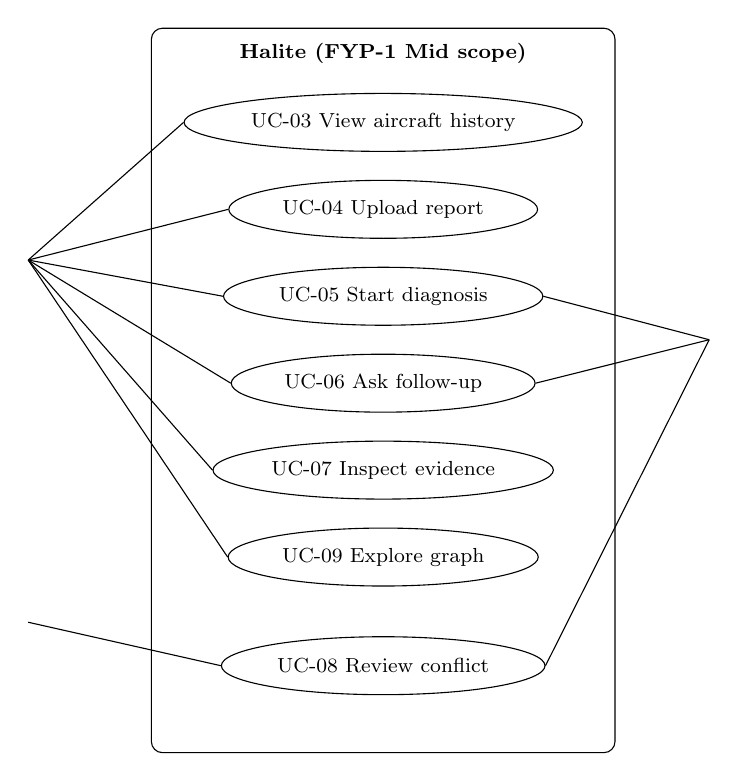
\begin{tikzpicture}[uc/.style={draw,ellipse,minimum width=3.5cm,minimum height=0.8cm,font=\footnotesize,align=center},>=Stealth,scale=0.92,transform shape]
\draw[rounded corners] (3.2,-3.4) rectangle (9.6,6.6);
\node[font=\footnotesize\bfseries] at (6.4,6.25) {Halite (FYP-1 Mid scope)};
\node[uc] (u3) at (6.4,5.3) {UC-03 View aircraft history};
\node[uc] (u4) at (6.4,4.1) {UC-04 Upload report};
\node[uc] (u5) at (6.4,2.9) {UC-05 Start diagnosis};
\node[uc] (u6) at (6.4,1.7) {UC-06 Ask follow-up};
\node[uc] (u7) at (6.4,0.5) {UC-07 Inspect evidence};
\node[uc] (u9) at (6.4,-0.7) {UC-09 Explore graph};
\node[uc] (u8) at (6.4,-2.2) {UC-08 Review conflict};
\stickman{0.9,3.3}{Maintenance\\technician}
\stickman{0.9,-1.8}{Maintenance\\supervisor}
\stickman{11.6,2.3}{Language model\\service (Groq)}
\foreach \u in {u3,u4,u5,u6,u7,u9} {\draw (1.5,3.4) -- (\u.west);}
\draw (1.5,-1.6) -- (u8.west);
\draw (10.9,2.3) -- (u5.east);
\draw (10.9,2.3) -- (u6.east);
\draw (10.9,2.3) -- (u8.east);
\end{tikzpicture}
\caption{Use case diagram. The language model service is a secondary actor: it phrases answers and proposes record classifications, but never decides a ranking. UC-05 and UC-08 both include UC-07: the user can open any cited record from them.}\label{fig:usecase}
\end{figure}

\section{Detailed Use Cases}
\subsection*{UC-03 View aircraft history}
\textbf{Actor:} technician. \textbf{Precondition:} records are loaded.\\
\textbf{Main flow:} (1) The technician opens Assets and sees each aircraft with its record count. (2) The technician searches by tail number or sorts by record count. (3) The technician opens an aircraft. (4) The system shows its records oldest first with the original FAA identifier, component, date and, where present, the analysis result.\\
\textbf{Alternative:} an unknown aircraft shows ``Aircraft not found'', not an empty history. A failed request shows an error with a retry action.\\
\textbf{Postcondition:} nothing is changed.

\subsection*{UC-04 Upload report}
\textbf{Actor:} technician. \textbf{Precondition:} a CSV in the FAA export format with \code{RegistryNNumber}, \code{DifficultyDate} (MM/DD/YYYY) and \code{OperatorControlNumber}.\\
\textbf{Main flow:} (1) The technician chooses a \code{.csv} file of at most 10~MB; nothing is sent yet. (2) The technician confirms ``Ingest this file''. (3) The system stores new records as unanalysed, skips invalid rows and duplicates, and returns counts. (4) The page shows the counts and a link to the new records.\\
\textbf{Alternative:} a non-CSV or oversize file is rejected before sending; an unreadable file produces an error message; re-uploading the same file reports every record as already stored.\\
\textbf{Postcondition:} new records exist as \code{unscored}; existing records are unchanged.

\subsection*{UC-05 Start diagnosis}
\textbf{Actor:} technician; secondary actor: language model. \textbf{Precondition:} an aircraft with history exists.\\
\textbf{Main flow:} (1) The technician selects an aircraft and enters a symptom. (2) The system validates the input and retrieves bounded graph context. (3) The system ranks inspection checks deterministically. (4) A live model phrases an explanation from the retrieved records only. (5) The system verifies every cited record identifier against the graph. (6) The interface shows the ranked checks, the explanation, the evidence records and the citation status.\\
\textbf{Alternative A:} no relevant history returns an explicit ``no relevant history'' result without invented records. \textbf{Alternative B:} no live model returns an HTTP 503 with a reason, and no diagnosis is shown. \textbf{Alternative C:} an identifier that does not exist is marked unverified.\\
\textbf{Postcondition:} nothing in the graph is changed.

\subsection*{UC-06 Ask follow-up}
As UC-05, with state carried between turns: the browser holds symptoms, observations, checks done, ruled-out components and open questions, and sends them with each message. The system re-ranks, reports which checks moved up or down, and asks at most one question. If the model is unavailable, the reply is empty but the ranking and evidence are still returned.

\subsection*{UC-07 Inspect evidence}
\textbf{Main flow:} the technician selects an evidence record identifier; the application opens that record on its aircraft's history page and marks it. \textbf{Alternative:} if the aircraft cannot be resolved, no link is shown and the identifier stays plain text.

\subsection*{UC-08 Review conflict}
\textbf{Actor:} maintenance supervisor. \textbf{Precondition:} the conflict engine has routed at least one record to review.\\
\textbf{Main flow:} (1) The supervisor opens the review queue. (2) The system shows the incoming record beside the retrieved prior record, with the classification, score and rationale. (3) The supervisor accepts, or rejects with a required note. (4) The system confirms with the server before changing the screen and stores the status, note and \code{reviewed} state.\\
\textbf{Alternative:} an action on a record that is no longer in a reviewable state returns a conflict error and leaves the queue unchanged. \textbf{Postcondition:} the source record is never deleted.

\section{Functional Requirements}
\textbf{Status key:} Met, Partial, Deferred. ``Check'' is the acceptance check.

\subsection{Module M02: Assets}
\begin{longtable}{p{0.08\textwidth}p{0.3\textwidth}p{0.4\textwidth}p{0.1\textwidth}}
\toprule \textbf{ID} & \textbf{Requirement} & \textbf{Acceptance check} & \textbf{Status} \\ \midrule \endhead
FR-05 & Register maintenance assets & Assets appear after ingest; no manual registration screen & Partial \\
FR-06 & Display chronological records for an asset & History for an aircraft lists its records oldest first; an unknown aircraft returns 404 & Met \\
FR-07 & Search assets by identifier & Typing part of a tail number filters the list & Met \\
FR-08 & Display record-linked diagnostic and conflict information & A corrected record shows its corrector; scores and states appear per record & Met \\
\bottomrule
\end{longtable}

\subsection{Module M03: Knowledge graph}
\begin{longtable}{p{0.08\textwidth}p{0.3\textwidth}p{0.4\textwidth}p{0.1\textwidth}}
\toprule \textbf{ID} & \textbf{Requirement} & \textbf{Acceptance check} & \textbf{Status} \\ \midrule \endhead
FR-13 & Create relationships among entities & After ingest every record has \code{ABOUT} to its aircraft and \code{PRECEDED_BY} to the earlier record on that aircraft & Met \\
FR-14 & Traverse related historical cases & The graph view shows one aircraft's records and the edges between them; counts equal the stored counts & Met \\
FR-15 & Expose provenance of graph results & The legend states which edges come from ingest and which are computed by the engine; a record shows its source & Met \\
\bottomrule
\end{longtable}

\subsection{Module M04: Diagnostics}
\begin{longtable}{p{0.08\textwidth}p{0.3\textwidth}p{0.4\textwidth}p{0.1\textwidth}}
\toprule \textbf{ID} & \textbf{Requirement} & \textbf{Acceptance check} & \textbf{Status} \\ \midrule \endhead
FR-16 & Accept natural-language symptoms & A Copilot message of 1 to 4000 characters is accepted; blank or longer input returns 422 & Met \\
FR-17 & Retrieve relevant historical evidence & Context is limited to the aircraft's recent history and a fleet scan capped at 2,500 records & Met (lexical) \\
FR-18 & Produce ranked hypotheses when evidence suffices & Ranking is deterministic: the same input gives the same order & Met (heuristic) \\
FR-19 & Display supporting record references & Each ranked check lists its record identifiers, each a link & Met \\
FR-20 & Ask for clarification when information is missing & The Copilot asks at most one question and tracks open questions & Partial \\
FR-21 & Distinguish unsupported from verified & Identifiers absent from the graph are marked unverified and omitted from the valid list & Met \\
FR-22 & Preserve diagnostic session history & Copilot sessions are saved in the browser only; no server-side history & Partial \\
\bottomrule
\end{longtable}

\subsection{Module M05: Conflict intelligence}
\begin{longtable}{p{0.08\textwidth}p{0.3\textwidth}p{0.4\textwidth}p{0.1\textwidth}}
\toprule \textbf{ID} & \textbf{Requirement} & \textbf{Acceptance check} & \textbf{Status} \\ \midrule \endhead
FR-23 & Compare new records with prior records & Candidates come only from the same aircraft, earlier in time, with at least one matching signal & Met \\
FR-24 & Classify potential conflicts & Each result is one of five labels; an unparseable reply routes to review & Met \\
FR-25 & Route uncertain cases for review & Contradicts and partially-supersedes always go to review; a supersession below the 0.50 threshold goes to review & Met \\
FR-26 & Record supervisor decisions & Accept stores status and note; reject requires a non-blank note & Met (no reviewer identity) \\
FR-27 & Audit trail of status changes & Status, review note and state are stored; no actor or event log & Partial \\
\bottomrule
\end{longtable}

\subsection{Module M06: Report intelligence}
\begin{longtable}{p{0.08\textwidth}p{0.3\textwidth}p{0.4\textwidth}p{0.1\textwidth}}
\toprule \textbf{ID} & \textbf{Requirement} & \textbf{Acceptance check} & \textbf{Status} \\ \midrule \endhead
FR-09 & Accept supported report formats & FAA-format CSV by upload or server path, and a single record form & Partial \\
FR-10 & Extract available fields & Tail, date, component, JASC code, location and text are stored & Partial \\
FR-11 & Retain the original source record & Text and identifier are stored unchanged; reject never deletes & Met \\
FR-12 & Flag ambiguous or invalid fields & Rows with no tail, a bad date or no identifier are counted separately & Partial \\
\bottomrule
\end{longtable}

\section{Non-Functional Requirements}
\subsection{Reliability}
\textbf{NFR-06:} failed external operations are reported and retried safely. \emph{Check:} a rate-limited model call is retried a bounded number of times; a missing live model returns 503 and never a stored stub as evidence; every page shows a failure state with a retry action and never an empty state that implies ``no data''. \emph{Status:} met, covered by the backfill, conflict-engine and component tests.

\subsection{Usability}
\textbf{NFR-08:} task completion and a usability score are measured. \emph{Status:} \textbf{not measured}; no user test was run. Design rules applied instead: errors name the cause, unanalysed records say so, scores carry their meaning, and destructive actions need confirmation.

\subsection{Performance}
\textbf{NFR-02:} non-generation requests meet a p95 of 500~ms. \emph{Measured:} the assets list took about 0.99~s as a single request on staging, \textbf{which exceeds the target}; no load test was run. The Service Records first load makes two page-initiated requests instead of 119. \textbf{NFR-03:} diagnostic latency is measured under a controlled workload; \emph{not measured}, because fresh diagnoses call an external model.

\subsection{Security}
\textbf{NFR-05} (no cross-tenant access) does not apply yet because there is no authentication or tenancy. What exists: the batch analysis and the log-retrieval endpoints need a secret operations token; secrets live in ignored environment files; the settings page no longer offers to wipe the graph. \textbf{Known risk:} \pth{DELETE /api/graph/reset} remains reachable without authentication (Section~\ref{sec:risks}).

\section{Acceptance Criteria}
The acceptance criteria are the checks above and the end-to-end acceptance tests T01 to T16 in Chapter~\ref{ch:testing}, which the team defined before the iteration.

\section{Requirements Traceability}
Table~\ref{tab:trace} traces the central requirements to their design, implementation and tests; the complete matrix is in Appendix~\ref{app:req}.

\begin{longtable}{p{0.1\textwidth}p{0.2\textwidth}p{0.3\textwidth}p{0.3\textwidth}}
\caption{Traceability of central requirements}\label{tab:trace}\\
\toprule \textbf{FR} & \textbf{Design element} & \textbf{Implementation} & \textbf{Tests} \\ \midrule \endfirsthead
\toprule \textbf{FR} & \textbf{Design element} & \textbf{Implementation} & \textbf{Tests} \\ \midrule \endhead
FR-06, 08 & Asset history API and page & \code{maintenance.py}, \code{AssetHistory.jsx} & \code{test_api_maintenance}; \code{AssetHistory.test} (12) \\
FR-13 & Graph schema, ingest & \code{maintenance_agent.py}, \code{queries.py} & \code{test_maintenance_agent} (10) \\
FR-14, 15 & Graph view & \code{Graph.jsx}, \code{graphScope.js} & \code{Graph.test} (18), \code{graphScope.test} (10) \\
FR-17, 18, 19 & Retrieval and ranking & \code{diagnostic_retrieval.py} & \code{test_diagnostic_retrieval} (26) \\
FR-21 & Citation validation & \code{citation_validation.py} & \code{test_citation_validation} (6) \\
FR-23, 24, 25 & Conflict engine & \code{conflict_engine.py} & \code{test_conflict_engine} (32), \code{test_conflict_cascade} (11) \\
FR-26 & Review actions & \code{maintenance.py}, \code{ReviewQueue.jsx} & \code{ReviewQueue.test} (18) \\
FR-09, 12 & CSV upload & \code{MaintenanceIngest.jsx}, \code{CsvUploader.jsx} & \code{MaintenanceIngest.test} (17) \\
\bottomrule
\end{longtable}

\chapter{System Design}\label{ch:design}

\section{System Architecture}
Halite is a client--server web application (Figure~\ref{fig:arch}). A React single-page application, hosted on Vercel, calls a FastAPI backend over JSON. The backend runs in Docker on a shared virtual machine and reads and writes a Neo4j graph database. A language model on the Groq API is called by the backend for three jobs only: phrasing an explanation, extracting structured facts from a technician's message in the multi-turn Copilot, and proposing a classification for a pair of records. The model never determines the diagnostic ranking.

\begin{figure}[htb]
\centering
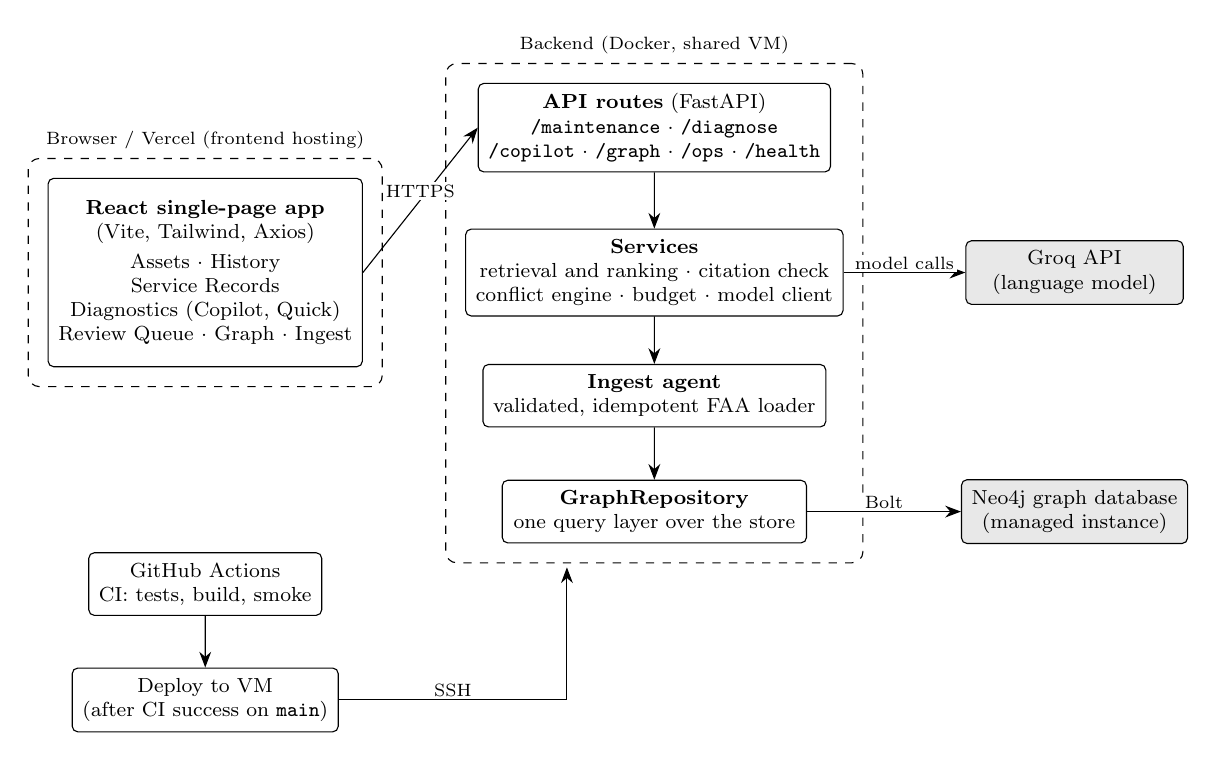
\begin{tikzpicture}[scale=0.92,transform shape]
\node[box,minimum width=3.7cm,minimum height=2.6cm] (ui) at (0,0) {\textbf{React single-page app}\\(Vite, Tailwind, Axios)\\[2pt]Assets $\cdot$ History\\Service Records\\Diagnostics (Copilot, Quick)\\Review Queue $\cdot$ Graph $\cdot$ Ingest};
\node[grp,fit=(ui),label={[font=\scriptsize]above:Browser / Vercel (frontend hosting)}] {};
\node[box,minimum width=4.2cm] (routes) at (6.2,2.0) {\textbf{API routes} (FastAPI)\\\code{/maintenance} $\cdot$ \code{/diagnose}\\\code{/copilot} $\cdot$ \code{/graph} $\cdot$ \code{/ops} $\cdot$ \code{/health}};
\node[box,minimum width=4.2cm] (svc) at (6.2,0) {\textbf{Services}\\retrieval and ranking $\cdot$ citation check\\conflict engine $\cdot$ budget $\cdot$ model client};
\node[box,minimum width=4.2cm] (agent) at (6.2,-1.7) {\textbf{Ingest agent}\\validated, idempotent FAA loader};
\node[box,minimum width=4.2cm] (repo) at (6.2,-3.3) {\textbf{GraphRepository}\\one query layer over the store};
\node[grp,fit=(routes)(svc)(agent)(repo),label={[font=\scriptsize]above:Backend (Docker, shared VM)}] {};
\node[ext,minimum width=3cm] (neo) at (12.0,-3.3) {Neo4j graph database\\(managed instance)};
\node[ext,minimum width=3cm] (groq) at (12.0,0) {Groq API\\(language model)};
\draw[arr] (ui.east) -- node[lab,above]{HTTPS} (routes.west);
\draw[arr] (routes) -- (svc);
\draw[arr] (svc) -- (agent);
\draw[arr] (agent) -- (repo);
\draw[arr] (repo.east) -- node[lab,above]{Bolt} (neo.west);
\draw[arr] (svc.east) -- node[lab,above]{model calls} (groq.west);
\node[box,minimum width=3.1cm] (ci) at (0,-4.3) {GitHub Actions\\CI: tests, build, smoke};
\node[box,minimum width=3.1cm] (dep) at (0,-5.9) {Deploy to VM\\(after CI success on \code{main})};
\draw[arr] (ci) -- (dep);
\draw[arr] (dep.east) -| node[lab,pos=0.25,above]{SSH} ([xshift=0.9cm,yshift=-0.33cm]repo.south west);
\end{tikzpicture}

\caption{System architecture and deployment path. Grey boxes are external services.}\label{fig:arch}
\end{figure}

\textbf{Runtime honesty.} \code{GET /api/health} reports the graph mode (\code{neo4j} or \code{memory}), whether the model is live, and the number of records loaded. The application and our evidence documents claim ``real data'' or ``live model'' only when this endpoint agrees. A \code{memory} mode exists for tests and degraded operation and is labelled as such.

\textbf{Domain registry.} Domain-specific rules (record labels, source authority) sit behind an adapter. The maintenance adapter is the product; the earlier software-engineering adapter is retained as frozen infrastructure, covered by seven regression tests, and is unreachable from the interface.

\section{Architectural Components}
\begin{longtable}{p{0.2\textwidth}p{0.4\textwidth}p{0.3\textwidth}}
\caption{Components and responsibilities}\label{tab:components}\\
\toprule \textbf{Component} & \textbf{Responsibility} & \textbf{Main files} \\ \midrule \endfirsthead
\toprule \textbf{Component} & \textbf{Responsibility} & \textbf{Main files} \\ \midrule \endhead
React application & Pages for assets, history, service records, diagnostics, review, graph, ingest; every failure state shown honestly & \code{frontend/src/pages}, \code{components}, \code{utils} \\
API client & One Axios instance and the functions for every endpoint & \pth{frontend/src/api/client.js} \\
API routes & HTTP contracts, validation, controlled errors (404, 409, 422, 503) & \code{backend/api/routes} \\
Ingest agent & Validated, idempotent loading of FAA records; explicit skip counts & \pth{agents/maintenance_agent.py} \\
Retrieval and ranking & Bounded graph context; deterministic ranking; copilot context and ranking delta & \pth{services/diagnostic_retrieval.py} \\
Citation validation & Extract FAA-shaped identifiers and check them against the graph & \pth{services/citation_validation.py} \\
Conflict engine & Candidate pairing, classification, adjudication, confidence, routing & \pth{services/conflict_engine.py}, \code{conflict_screen.py} \\
Analysis state and budget & Honest unanalysed state; per-day request and token budget & \code{analysis_state.py}, \code{analysis_budget.py} \\
Model client & Calls Groq; rejects empty content; bounded retries & \pth{services/groq_service.py} \\
Graph repository & One query layer over Neo4j or the in-memory store & \code{graph/queries.py}, \code{schema.py} \\
\bottomrule
\end{longtable}

\section{Interfaces and Dependencies}
\subsection{Backend interfaces}
\begin{longtable}{p{0.1\textwidth}p{0.36\textwidth}p{0.44\textwidth}}
\caption{Principal backend endpoints}\label{tab:api}\\
\toprule \textbf{Method} & \textbf{Path} & \textbf{Purpose and contract notes} \\ \midrule \endfirsthead
\toprule \textbf{Method} & \textbf{Path} & \textbf{Purpose and contract notes} \\ \midrule \endhead
GET & \code{/api/health} & Runtime mode and record count \\
GET & \pth{/api/maintenance/assets} & Aircraft with record counts, one aggregation query \\
GET & \code{/api/maintenance/assets/{id}/history} & One aircraft's records; keyed by the aircraft UUID; unknown returns 404 \\
GET & \pth{/api/maintenance/records} & Fleet-wide list: filters, deterministic pagination \\
POST & \pth{/api/maintenance/records} & Submit one record and process it \\
POST & \pth{/api/maintenance/ingest} & Ingest a CSV already on the server \\
POST & \pth{/api/maintenance/ingest/upload} & Multipart CSV upload, same ingest \\
GET & \pth{/api/maintenance/review-queue} & Records awaiting review \\
POST & \code{/api/maintenance/review-queue/{id}/accept} or \code{/reject} & Review action; reject needs a note; 409 if not reviewable \\
GET & \pth{/api/maintenance/corrections} & One row per \code{SUPERSEDES} edge with a summary \\
GET & \pth{/api/maintenance/analysis/status} & Analysis coverage and label counts \\
POST & \pth{/api/maintenance/analysis/run} & Batch analysis, at most 25 records; needs the operations token and a live model \\
POST & \pth{/api/maintenance/diagnose} & One-shot diagnosis; 404 unknown or empty history; 503 if the model is unavailable \\
POST & \pth{/api/maintenance/copilot/turn} & Multi-turn copilot; state carried by the client \\
GET & \code{/api/graph/overview} & Nodes and edges for the graph view; \code{limit} sets the node cap (default 200) \\
GET & \code{/api/ops/version}, \code{/api/ops/logs} & Deployed commit; recent log lines (token required) \\
DELETE & \code{/api/graph/reset} & Wipes the graph. Needs the operations token (503 if none is configured) and, for Neo4j, \code{confirm=WIPE} \\
\bottomrule
\end{longtable}

\subsection{Component dependencies}
Figure~\ref{fig:components} shows which module calls which. Routes call services; services call one repository; the repository is the only code that talks to the database. This keeps the graph queries in one place and lets the same service code run against an in-memory store in tests.

\begin{figure}[htb]
\centering
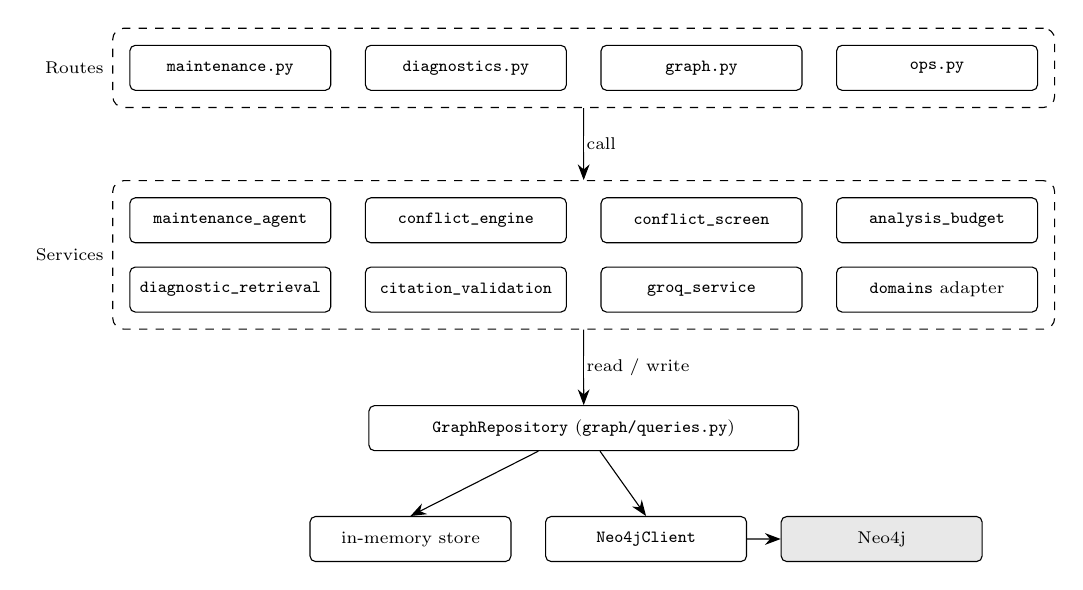
\begin{tikzpicture}[scale=0.88,transform shape,cb/.style={draw,rounded corners=2pt,font=\scriptsize,minimum width=2.9cm,minimum height=0.65cm,align=center,fill=white}]
% layer 1: routes
\foreach \x/\k/\n in {0/a/maintenance.py,3.4/b/diagnostics.py,6.8/c/graph.py,10.2/d/ops.py} {\node[cb] (r\k) at (\x,0) {\texttt{\n}};}
\node[draw,dashed,rounded corners=4pt,fit=(ra)(rb)(rc)(rd),inner sep=6pt,label={[font=\scriptsize]left:Routes}] (L1) {};
% layer 2: services
\node[cb] (s1) at (0,-2.2) {\code{maintenance_agent}};
\node[cb] (s2) at (3.4,-2.2) {\code{conflict_engine}};
\node[cb] (s3) at (6.8,-2.2) {\code{conflict_screen}};
\node[cb] (s4) at (10.2,-2.2) {\code{analysis_budget}};
\node[cb] (s5) at (0,-3.2) {\code{diagnostic_retrieval}};
\node[cb] (s6) at (3.4,-3.2) {\code{citation_validation}};
\node[cb] (s7) at (6.8,-3.2) {\code{groq_service}};
\node[cb] (s8) at (10.2,-3.2) {\code{domains} adapter};
\node[draw,dashed,rounded corners=4pt,fit=(s1)(s2)(s3)(s4)(s5)(s6)(s7)(s8),inner sep=6pt,label={[font=\scriptsize]left:Services}] (L2) {};
% layer 3
\node[cb,minimum width=6.2cm] (repo) at (5.1,-5.2) {\code{GraphRepository} (\code{graph/queries.py})};
% layer 4
\node[cb] (mem) at (2.6,-6.8) {in-memory store};
\node[cb] (n4j) at (6.0,-6.8) {\code{Neo4jClient}};
\node[cb,fill=gray!18] (db) at (9.4,-6.8) {Neo4j};
\draw[arr] (L1.south) -- node[lab,right]{call} (L2.north);
\draw[arr] (L2.south) -- node[lab,right]{read / write} (repo.north);
\draw[arr] (repo) -- (mem.north); \draw[arr] (repo) -- (n4j.north); \draw[arr] (n4j)--(db);
\end{tikzpicture}

\caption{Backend component dependencies.}\label{fig:components}
\end{figure}

\subsection{External dependencies}
Neo4j (graph database), Groq (language model), FastAPI and Pydantic, pandas (CSV loading), React 18, Vite, Tailwind CSS, Axios, \code{react-force-graph-3d}, Vitest, PyTest, Docker Compose, GitHub Actions and Vercel. Section~\ref{sec:external} gives the list with versions and purpose.

\section{Architecture Decisions and Rationale}
Non-obvious decisions are recorded as short decision records in the repository. Table~\ref{tab:dec} lists those most relevant to this iteration.
\begin{longtable}{p{0.3\textwidth}p{0.62\textwidth}}
\caption{Selected architecture and process decisions}\label{tab:dec}\\
\toprule \textbf{Decision (date)} & \textbf{Rationale} \\ \midrule \endfirsthead
\toprule \textbf{Decision (date)} & \textbf{Rationale} \\ \midrule \endhead
Maintenance-only frontend (16 Oct) & The product is maintenance diagnostics; the legacy software screens stay in the repository but are unreachable, so they cannot be mistaken for features \\
Frontend reflects backend outputs (16 Oct) & The interface may add labels and warnings but must never hide, alter or invent a value the backend returned \\
Review actions are server-confirmed (16 Oct) & Accept and reject change real data, so the screen changes only after the server confirms; no keyboard shortcut can trigger them \\
Centralised staging and CI-gated release (16 Oct) & One shared staging API for the whole team; only a commit that passed full CI on \code{main} is deployed, with a recorded rollback \\
Honest analysis state (17 Oct) & Analysis state is stored separately from confidence; ``unscored'' is never shown as a confident result \\
Fleet-wide paginated records (17 Oct) & Replaced a 119-request fan-out with one paginated, filterable endpoint \\
Opt-in cost cascade (17 Oct) & Pre-registered, off by default: a deterministic text screen before the model, and adaptive voting, to cut requests without tuning against the evaluation \\
Diagnostic copilot scope waiver (16 Oct) & A named, limited exception to file ownership so the copilot could be built across route, retrieval and UI without touching the conflict engine, ingest or CI \\
Graph shows one aircraft (17 Oct) & The whole graph is too dense to read; one aircraft's stored subgraph is readable and every drawn edge is a stored edge \\
Graph reset protected (18 Oct) & A destructive route had no authentication; it now needs the operations token and a typed confirmation, and regression tests prove an unauthenticated call changes nothing \\
Knowledge bank and agent protocol (16 Oct) & A written, versioned memory of context, flows and decisions that every contributor and every AI assistant must read first and update in the same change \\
\bottomrule
\end{longtable}

\section{Design Evolution}
\begin{longtable}{p{0.22\textwidth}p{0.3\textwidth}p{0.4\textwidth}}
\caption{Design as proposed against design as built}\label{tab:evolution}\\
\toprule \textbf{Aspect} & \textbf{Proposal} & \textbf{Built at Mid, and why} \\ \midrule \endfirsthead
\toprule \textbf{Aspect} & \textbf{Proposal} & \textbf{Built at Mid, and why} \\ \midrule \endhead
Retrieval & Graph-constrained plus embedding-based hybrid & Graph-bounded with lexical (Jaccard) similarity; embeddings deferred so the baseline is measured first \\
Ranking & Hybrid evidence score with a historical correction penalty & Deterministic: recency and similarity weights, factor 0.3 for superseded records \\
Conflict engine & Five-label classifier with human review & As proposed; plus a stored analysis state, a daily budget, and an opt-in cost cascade after we measured 9,175 projected requests \\
Tenancy and identity & PostgreSQL, organisations, roles & Not built; reviewer identity is therefore not recorded \\
Sessions & Server-side diagnostic session storage & Client-side state only; the server is stateless \\
Interface & Chat-centred workspace & Asset-first workspace with a Copilot tab; one-shot diagnose kept as the stable contract \\
Corpus & About 60 airframes & 118 aircraft, because every aircraft with a ground-truth pair is kept first \\
\bottomrule
\end{longtable}

\section{Domain Model}
Figure~\ref{fig:erd} is the graph schema. There are two node types and three relationship types. Each relationship records its provenance: \code{ABOUT} and \code{PRECEDED_BY} are created at ingest; \code{SUPERSEDES} is created only by the conflict engine when a supersession is confirmed. No relationship is invented to make the graph look richer; a causal ``component causes failure'' edge is deliberately absent because the data does not justify one.

\begin{figure}[htb]
\centering
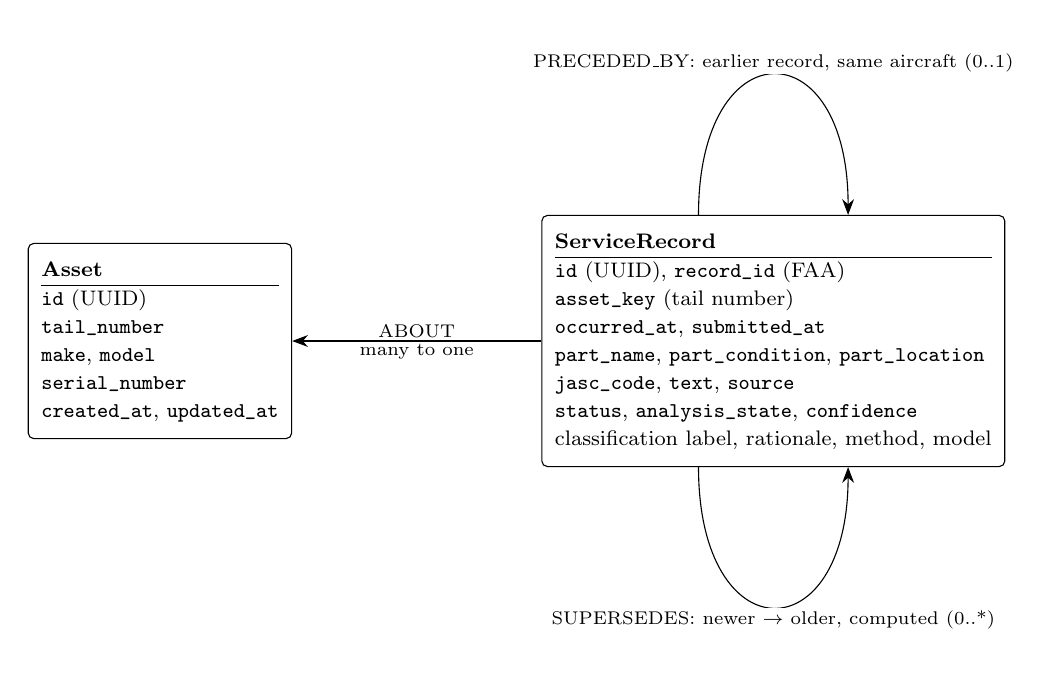
\begin{tikzpicture}[scale=0.95,transform shape]
\node[draw,rounded corners=2pt,align=left,font=\footnotesize,inner sep=5pt] (asset) at (0,0) {\begin{tabular}{@{}l@{}}\textbf{Asset}\\\hline \code{id} (UUID)\\ \code{tail_number}\\ \code{make}, \code{model}\\ \code{serial_number}\\ \code{created_at}, \code{updated_at}\end{tabular}};
\node[draw,rounded corners=2pt,align=left,font=\footnotesize,inner sep=5pt] (sr) at (8.2,0) {\begin{tabular}{@{}l@{}}\textbf{ServiceRecord}\\\hline \code{id} (UUID), \code{record_id} (FAA)\\ \code{asset_key} (tail number)\\ \code{occurred_at}, \code{submitted_at}\\ \code{part_name}, \code{part_condition}, \code{part_location}\\ \code{jasc_code}, \code{text}, \code{source}\\ \code{status}, \code{analysis_state}, \code{confidence}\\ classification label, rationale, method, model\end{tabular}};
\draw[arr] (sr.west) -- node[lab,above]{ABOUT} node[lab,below]{many to one} (asset.east);
\draw[arr] ([xshift=-1cm]sr.north) to[out=90,in=90,looseness=3.2] node[above,lab,pos=0.5]{PRECEDED\_BY: earlier record, same aircraft (0..1)} ([xshift=1cm]sr.north);
\draw[arr] ([xshift=-1cm]sr.south) to[out=-90,in=-90,looseness=3.2] node[below,lab,pos=0.5]{SUPERSEDES: newer $\rightarrow$ older, computed (0..*)} ([xshift=1cm]sr.south);
\end{tikzpicture}

\caption{Graph schema (entity--relationship view).}\label{fig:erd}
\end{figure}

\section{Data Design}\label{sec:data}
\textbf{Source.} FAA Service Difficulty Reports, 2025 file: 67,637 raw rows, 66,658 after removing duplicates on (aircraft, date, normalised text). The proof-of-concept corpus is a deterministic selection (fixed seed): every aircraft that has a ground-truth pair is included first, then others are added until about 2,000 records. It holds \textbf{2,079 records on 118 aircraft}; the largest aircraft has 153 records. Raw and processed files are not committed; a script downloads them \citep{faa-sdr}.

\textbf{Ground truth.} 141 valid correction pairs written by the FAA reporters (``supplemental report for \ldots'') were extracted; six candidates were discarded (five cite a record outside the corpus, one crosses aircraft).

\textbf{Ingest rules.} A row needs a tail number, a parseable \code{MM/DD/YYYY} date and an \code{OperatorControlNumber}; otherwise it is counted in a named skip category. A record that already exists is counted as a duplicate and left unchanged, and its \code{ABOUT} link is re-asserted so an interrupted earlier run is repaired. New records are stored with status \code{unscored}, \code{analysis_state} \code{unscored} and a null confidence.

\textbf{Status values.} Workflow \code{status}: \code{unscored}, \code{no_action}, \code{auto_accepted}, \code{needs_review}, \code{accepted}, \code{rejected}, \code{superseded}. Coverage \code{analysis_state}: \code{unscored}, \code{scored}, \code{needs_review}, \code{reviewed}. The two are separate on purpose: whether a record has been analysed is not the same as what the analysis decided.

\textbf{Known data fact.} On staging, 2,079 record nodes have 2,078 \code{ABOUT} links: one record (\code{AALA202506230216}, aircraft 991AU) is an orphan. Re-running ingest repairs it, but staging was not mutated without approval.

\section{Process / Behavior Design}
\subsection{Diagnosis}
Figure~\ref{fig:seq} shows the one-shot diagnosis. The retrieval and ranking happen before the model is called, so the ranking is identical with or without a model. If the model is unavailable, or returns empty text, the route returns HTTP 503 with a reason and the interface shows no diagnosis. After the model answers, every identifier in its text is looked up in the graph.

\begin{figure}[htb]
\centering
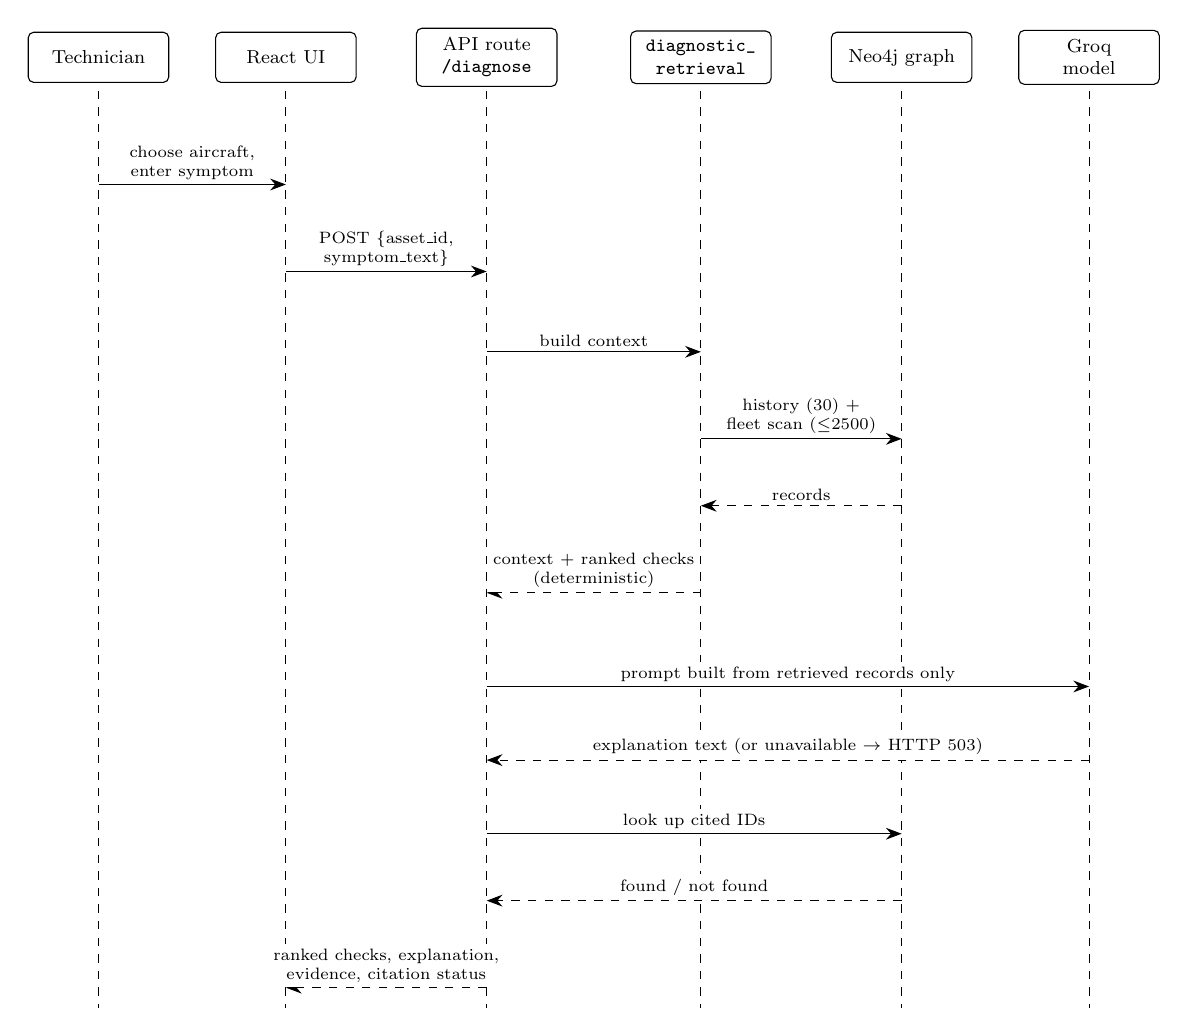
\begin{tikzpicture}[scale=0.85,transform shape]
\newcommand{\msg}[5]{\draw[#5] (#2,#1)--node[above,fill=white,font=\scriptsize,align=center,inner sep=2pt]{#4}(#3,#1);}
\foreach \x/\n in {0/Technician,2.8/React UI,5.8/{API route\\\code{/diagnose}},9.0/{\code{diagnostic_}\\\code{retrieval}},12.0/Neo4j graph,14.8/{Groq\\model}} {
  \node[box,minimum width=2.1cm] at (\x,0) {\n};
  \draw[dashed] (\x,-0.5)--(\x,-14.2);
}
\msg{-1.9}{0}{2.8}{choose aircraft,\\enter symptom}{arr}
\msg{-3.2}{2.8}{5.8}{POST \{asset\_id,\\symptom\_text\}}{arr}
\msg{-4.4}{5.8}{9.0}{build context}{arr}
\msg{-5.7}{9.0}{12.0}{history (30) +\\fleet scan ($\le$2500)}{arr}
\msg{-6.7}{12.0}{9.0}{records}{darr}
\msg{-8.0}{9.0}{5.8}{context + ranked checks\\(deterministic)}{darr}
\msg{-9.4}{5.8}{14.8}{prompt built from retrieved records only}{arr}
\msg{-10.5}{14.8}{5.8}{explanation text (or unavailable $\to$ HTTP 503)}{darr}
\msg{-11.6}{5.8}{12.0}{look up cited IDs}{arr}
\msg{-12.6}{12.0}{5.8}{found / not found}{darr}
\msg{-13.9}{5.8}{2.8}{ranked checks, explanation,\\evidence, citation status}{darr}
\end{tikzpicture}

\caption{Sequence diagram: one-shot diagnosis. Dashed arrows are returns.}\label{fig:seq}
\end{figure}

\subsection{Conflict analysis}
Figure~\ref{fig:flow} is the conflict pipeline. Only the leftmost path calls the model. Records with no comparable earlier record, and (in cascade mode) pairs the deterministic screen rules out, never reach it.

\begin{figure}[htb]
\centering
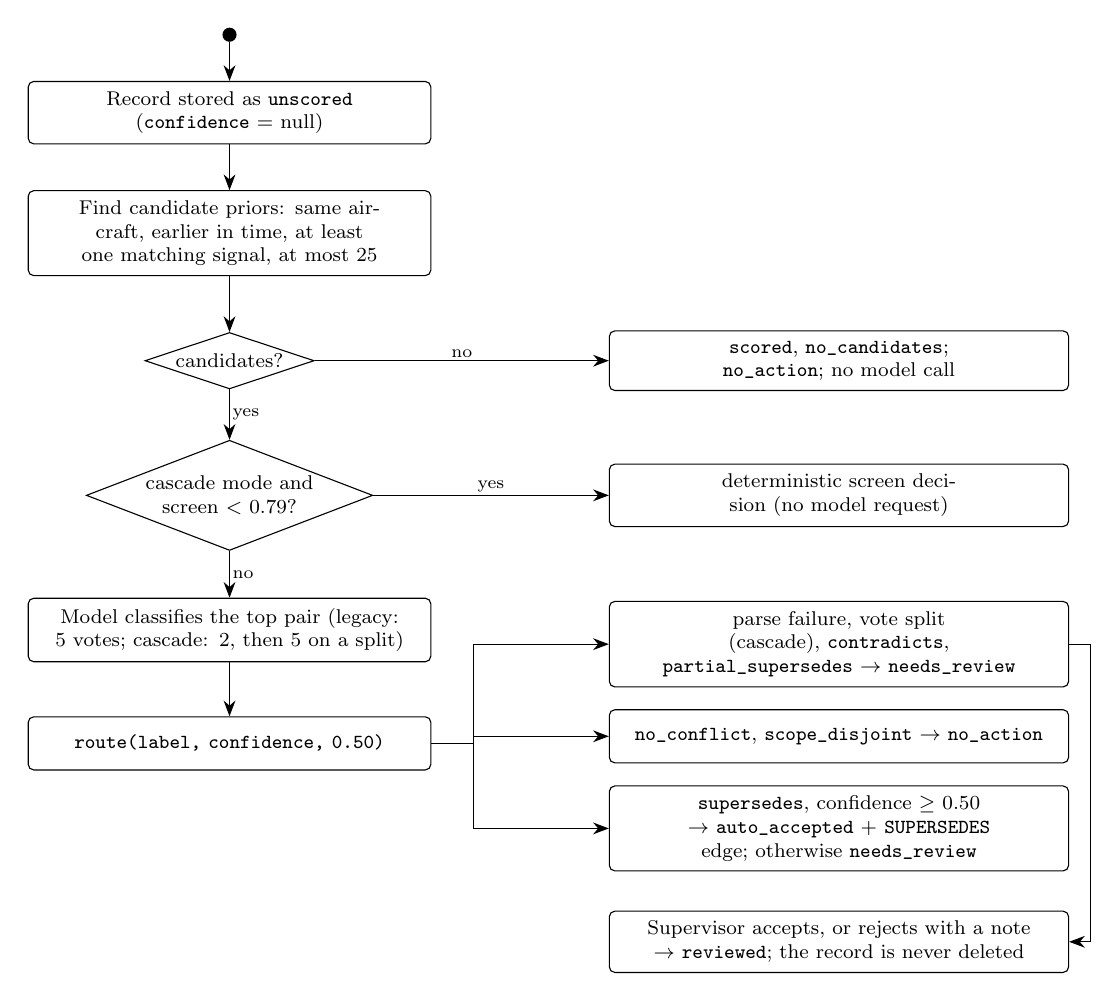
\begin{tikzpicture}[scale=0.9,transform shape,wbox/.style={box,text width=5.4cm},rbox/.style={box,text width=6.2cm}]
\node[circle,fill=black,inner sep=2pt] (s) at (0,0) {};
\node[wbox] (a) at (0,-1.1) {Record stored as \code{unscored}\\(\code{confidence} = null)};
\node[wbox] (b) at (0,-2.8) {Find candidate priors: same aircraft, earlier in time, at least one matching signal, at most 25};
\node[diamond,draw,aspect=3,font=\footnotesize,align=center,inner sep=1pt] (d1) at (0,-4.6) {candidates?};
\node[rbox] (o1) at (8.6,-4.6) {\code{scored}, \code{no_candidates}; \code{no_action}; no model call};
\node[diamond,draw,aspect=2.6,font=\footnotesize,align=center,inner sep=1pt] (d2) at (0,-6.5) {cascade mode and\\screen $<$ 0.79?};
\node[rbox] (o2) at (8.6,-6.5) {deterministic screen decision (no model request)};
\node[wbox] (c) at (0,-8.4) {Model classifies the top pair (legacy: 5 votes; cascade: 2, then 5 on a split)};
\node[wbox] (r) at (0,-10.0) {\code{route(label, confidence, 0.50)}};
\node[rbox] (n1) at (8.6,-8.6) {parse failure, vote split (cascade), \code{contradicts}, \code{partial_supersedes} $\to$ \code{needs_review}};
\node[rbox] (n2) at (8.6,-9.9) {\code{no_conflict}, \code{scope_disjoint} $\to$ \code{no_action}};
\node[rbox] (n3) at (8.6,-11.2) {\code{supersedes}, confidence $\ge$ 0.50 $\to$ \code{auto_accepted} + \code{SUPERSEDES} edge; otherwise \code{needs_review}};
\node[rbox] (rv) at (8.6,-12.8) {Supervisor accepts, or rejects with a note $\to$ \code{reviewed}; the record is never deleted};
\draw[arr] (s)--(a); \draw[arr] (a)--(b); \draw[arr] (b)--(d1);
\draw[arr] (d1.east)-- node[lab,above]{no} (o1.west);
\draw[arr] (d1)-- node[lab,right]{yes} (d2);
\draw[arr] (d2.east)-- node[lab,above]{yes} (o2.west);
\draw[arr] (d2)-- node[lab,right]{no} (c);
\draw[arr] (c)--(r);
\draw (r.east) -- ++(0.6,0) coordinate (bus);
\draw[arr] (bus) |- (n1.west); \draw[arr] (bus) |- (n2.west); \draw[arr] (bus) |- (n3.west);
\draw[arr] (n1.east) -- ++(0.3,0) |- (rv.east);
\end{tikzpicture}

\caption{Activity diagram: analysis of one record.}\label{fig:flow}
\end{figure}

\subsection{Record state}
Figure~\ref{fig:states} shows how the two state fields change. A record's \code{status} becomes \code{superseded} only when a later record's supersession is confirmed.

\begin{figure}[htb]
\centering
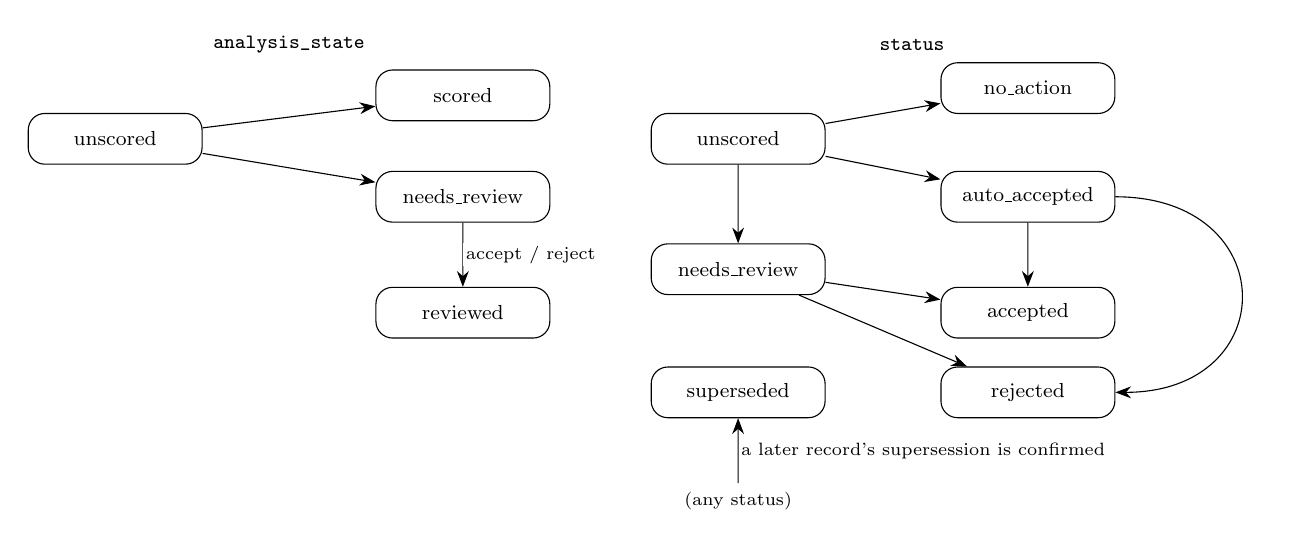
\begin{tikzpicture}[scale=0.92,transform shape,st/.style={draw,rounded corners=6pt,font=\footnotesize,minimum width=2.4cm,minimum height=0.7cm,align=center,fill=white}]
\node[font=\footnotesize\bfseries] at (2.4,2.1) {\code{analysis_state}};
\node[st] (u) at (0,0.8) {unscored};
\node[st] (sc) at (4.8,1.4) {scored};
\node[st] (nr) at (4.8,0) {needs\_review};
\node[st] (rv) at (4.8,-1.6) {reviewed};
\draw[arr] (u)--(sc); \draw[arr] (u)--(nr); \draw[arr] (nr)--node[lab,right]{accept / reject}(rv);
\node[font=\footnotesize\bfseries] at (11.0,2.1) {\code{status}};
\node[st] (su) at (8.6,0.8) {unscored};
\node[st] (na) at (12.6,1.5) {no\_action};
\node[st] (aa) at (12.6,0) {auto\_accepted};
\node[st] (nr2) at (8.6,-1.0) {needs\_review};
\node[st] (ac) at (12.6,-1.6) {accepted};
\node[st] (rj) at (12.6,-2.7) {rejected};
\node[st] (sp) at (8.6,-2.7) {superseded};
\draw[arr] (su)--(na); \draw[arr] (su)--(aa); \draw[arr] (su)--(nr2);
\draw[arr] (nr2)--(ac); \draw[arr] (nr2)--(rj); \draw[arr] (aa)--(ac); \draw[arr] (aa.east) to[out=0,in=0,looseness=2.2] (rj.east);
\node[font=\scriptsize] (any) at (8.6,-4.2) {(any status)};
\draw[arr] (any) -- node[lab,right]{a later record's supersession is confirmed} (sp);
\end{tikzpicture}

\caption{State diagrams for \texttt{analysis\_state} and \texttt{status}.}\label{fig:states}
\end{figure}

\subsection{Build and release}
Figure~\ref{fig:cicd} shows how a change reaches users. The frontend is built by Vercel on every push. The backend is deployed to staging only from a \code{main} commit that passed all three CI jobs; a manual deploy or rollback needs an exact commit and a typed confirmation.

\begin{figure}[htb]
\centering
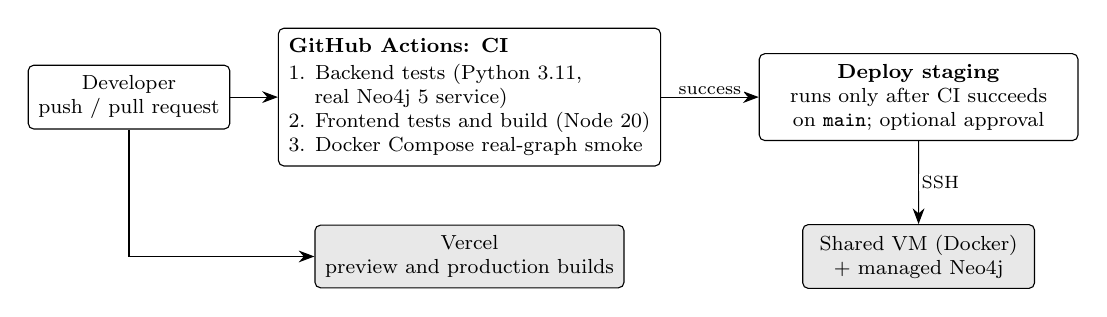
\begin{tikzpicture}[scale=0.92,transform shape]
\node[box,minimum width=2.6cm] (dev) at (0,0) {Developer\\push / pull request};
\node[box,minimum width=4.2cm,align=left] (ci) at (4.7,0) {\textbf{GitHub Actions: CI}\\[1pt]1. Backend tests (Python 3.11,\\\hspace{1.2em}real Neo4j 5 service)\\2. Frontend tests and build (Node 20)\\3. Docker Compose real-graph smoke};
\node[box,minimum width=4.4cm] (dep) at (10.9,0) {\textbf{Deploy staging}\\runs only after CI succeeds\\on \code{main}; optional approval};
\node[ext,minimum width=3.2cm] (vm) at (10.9,-2.2) {Shared VM (Docker)\\+ managed Neo4j};
\node[ext,minimum width=3.2cm] (vc) at (4.7,-2.2) {Vercel\\preview and production builds};
\draw[arr] (dev)--(ci); \draw[arr] (ci)--node[lab,above]{success}(dep); \draw[arr] (dep)--node[lab,right]{SSH}(vm);
\draw[arr] (dev) |- (vc.west);
\end{tikzpicture}

\caption{CI/CD pipeline.}\label{fig:cicd}
\end{figure}

\chapter{Iteration 1: Design and Implementation}\label{ch:iter1}

\section{Iteration Objectives}
Deliver a working vertical slice on real data: a technician selects a real aircraft, reads its dated records, enters a symptom, receives a ranked, evidence-linked investigation, opens a cited record, and sees a real correction or conflict. The same commit has automated tests and a continuous-integration run, and every failure path is reported honestly.

\section{Selected Use Cases / Features}
UC-03 (view history), UC-04 (upload report), UC-05 (start diagnosis), UC-06 (ask follow-up), UC-07 (inspect evidence), UC-08 (review conflict) and UC-09 (explore graph), as defined in Chapter~\ref{ch:req}.

\section{Design}
The design is in Chapter~\ref{ch:design}. Three iteration-specific design rules governed the work:
\begin{enumerate}
\item \textbf{The interface reflects the backend and never improves on it.} It may add labels and warnings; it may not hide, alter or invent a value.
\item \textbf{Real data or a stated reason.} A missing live model or graph is reported, never replaced by a stub that looks like a result.
\item \textbf{One owner per file, contracts frozen.} The diagnose request and response were fixed early so that three people could build in parallel.
\end{enumerate}

\section{Implementation}\label{sec:setup}
\subsection{Reproducing the system}
The full guide is \code{docs/mid1_setup.md}. In outline, with Docker, Python 3.11 and Node 20:
\begin{lstlisting}
# 1. Graph database
docker compose up -d neo4j
# 2. Backend (environment values, never committed, go in backend/.env)
cd backend && python -m venv venv && . venv/bin/activate
pip install -r requirements.txt
python scripts/fetch_sdr_data.py          # downloads the FAA 2025 file, builds the corpus
uvicorn main:app --port 8000               # DEMO_MODE=false, NEO4J_URI, NEO4J_PASSWORD, GROQ_API_KEY
curl -X POST localhost:8000/api/maintenance/ingest   # loads 2,079 records
# 3. Frontend
cd ../frontend && npm ci && npm run dev    # http://localhost:5173
# 4. Checks
cd ../backend && python -m pytest -q
cd ../frontend && npm test && npm run build
\end{lstlisting}
\code{GET /api/health} must report \code{graph_mode: neo4j} and a non-zero record count before any claim of ``real data'' is made. A Docker Compose smoke test in CI starts the whole stack and checks health, the corpus and the maintenance APIs. We have not yet had a person outside the team follow the guide on a clean machine (acceptance test T15).

\subsection{Repository layout}
\begin{longtable}{p{0.3\textwidth}p{0.6\textwidth}}
\toprule \textbf{Path} & \textbf{Content} \\ \midrule \endhead
\code{backend/api/routes} & HTTP routes \\
\code{backend/services} & Retrieval, ranking, citation check, conflict engine, budget, model client \\
\code{backend/agents} & Ingest agent \\
\code{backend/graph} & Schema, repository (queries), Neo4j client, in-memory store \\
\code{backend/tests} & 194 PyTest tests \\
\code{frontend/src} & Pages, components, hooks, utilities, API client; 171 Vitest tests in \code{src/test} \\
\code{knowledge/} & Context, flows, decision records \\
\code{docs/mid1/} & Dated evidence: audits, measurements, screenshots \\
\code{.github/workflows} & CI, staging deployment, log retrieval \\
\bottomrule
\end{longtable}

\section{Completed Features / Module}
\begin{description}
\item[M02 Assets.] \code{Assets} lists 118 aircraft with record counts from one aggregation query, searchable by tail number. \code{AssetHistory} shows an aircraft's records oldest first with identifiers, a ``Corrected by'' banner when a later record supersedes one, and deep links (\code{#recordId}) that scroll to and mark a record. \code{ServiceRecords} is a fleet-wide, URL-backed, paginated list with filters for text, status, analysis state, component and date.
\item[M03 Knowledge graph.] \code{Graph} loads the stored graph and shows one aircraft's subgraph: the aircraft, its records, and the edges between them. It states the true counts and draws \code{SUPERSEDES} apart from the other edges, with a legend that says where each comes from. A fallback for browsers without WebGL is in an open pull request and is not part of the commit this report cites.
\item[M04 Diagnostics.] \code{Diagnostics} has a multi-turn Copilot and a one-shot ``Quick diagnose''. Both show the ranked checks, the evidence records (each a link), the model's explanation when one exists, and the citation status.
\item[M05 Conflict intelligence.] \code{ReviewQueue} shows the incoming record beside the retrieved prior record with the label, score and rationale, and offers accept and reject. A second tab lists detected corrections with a component-change rate.
\item[M06 Report intelligence.] \code{MaintenanceIngest} uploads a CSV (explicit confirmation step, backend counts) or submits one record.
\end{description}

\section{Technical Implementation Details}
\subsection{Ingest}
\code{MaintenanceAgent} reads the CSV with every column as a string (a tail number such as \code{26226} must not become an integer). For each row it checks the tail, the date and the identifier, finds or creates the \code{Asset}, skips a record whose identifier already exists (re-asserting its \code{ABOUT} link), creates the \code{ServiceRecord} as unscored, links it to its aircraft, and links it to the previous record on that aircraft with \code{PRECEDED_BY}, in date order. It returns counts: records created, duplicates skipped, rows skipped for no tail, and rows skipped for a bad date or missing identifier.

\subsection{Retrieval and ranking}\label{sec:alg-rank}
\textbf{Context.} For a diagnosis the backend takes the aircraft's most recent records (default 30) and scans up to 2,500 records from other aircraft. Each fleet record is scored by
\[
s_{\text{fleet}} = 0.5\,[\text{JASC code equal}] + 0.3\,J(\text{symptom},\text{part name}) + 0.2\,J(\text{symptom},\text{record text}),
\]
where $J$ is the Jaccard similarity of the two word sets \citep{jaccard1912}; records scoring below 0.05 are dropped and the best 20 are kept.

\textbf{Ranking.} Each component (part name) receives the sum of its evidence weights:
\[
\text{score}(c) = \sum_{i\in H_c} \frac{0.4}{i+1}\,p_i \;+\; \sum_{r\in F_c} 0.6\, s_{\text{fleet}}(r)\, p_r ,
\qquad p = \begin{cases}0.3 & \text{record superseded}\\ 1 & \text{otherwise}\end{cases}
\]
with $H_c$ the aircraft's own recent records for component $c$ (position $i$ counted from the newest, starting at 0) and $F_c$ the fleet matches. Ties are broken by evidence count (higher first), then by component name, so the order is the same on every run. The weights (0.4, 0.6, 0.3) are constants chosen by the team and are not fitted to data; the score is a ranking aid, not a probability, and the interface says so.

\textbf{Copilot.} The Copilot repeats retrieval over all symptoms and observations the user has accumulated, excludes components the user has ruled out, excludes superseded records from recommendations (they stay visible as evidence), and reports which checks moved up, moved down, appeared or dropped since the previous turn.

\subsection{Citation validation}
Every token shaped like an FAA identifier (two to six capital letters followed by at least six digits) in the model's text is looked up in the graph. Those found are \code{valid}; the rest are \code{invalid} and are wrapped as \code{[UNVERIFIED:id]} in the displayed text. This confirms that a record exists; it does not confirm that the sentence citing it is supported, and the interface says that too.

\subsection{Conflict engine}
\textbf{Candidates.} For a record $r$ on aircraft $a$, every earlier record on $a$ is scored: \code{same part name} +3, \code{same JASC code} +2, \code{same location} +1, \code{within 30 days} +1. Only records with a positive score are candidates; ties are ordered by date (newest first) and identifier; at most 25 are kept. Records from the future are never compared, which prevents leakage.

\textbf{Classification.} The model returns a label (\code{no_conflict}, \code{scope_disjoint}, \code{supersedes}, \code{partial_supersedes}, \code{contradicts}) and a one-sentence rationale for the top candidate. An unparseable reply is flagged and routed to review.

\textbf{Confidence.} Signals are summed with weights that depend on whether the new record contains the FAA phrase ``SUPPLEMENTAL REPORT FOR'':
\begin{center}
\begin{tabular}{lcc}
\toprule \textbf{Signal} & \textbf{With phrase} & \textbf{Without} \\ \midrule
Explicit supersession language & 0.40 & 0 \\
Model says supersedes / partially & 0.20 & 0.35 \\
New record is clearly later & 0.15 & 0.25 \\
Source authority not lower & 0.10 & 0.15 \\
Same part and JASC code & 0.10 & 0.15 \\
Within 30 days & 0.05 & 0.10 \\
\bottomrule
\end{tabular}
\end{center}
The result is clamped to $[0,1]$. In cascade mode the model signal is scaled by vote agreement.

\textbf{Routing.} An unparseable reply, \code{contradicts} and \code{partial_supersedes} always go to review; \code{no_conflict} and \code{scope_disjoint} need no action; \code{supersedes} is accepted automatically only when confidence reaches the threshold 0.50, which the earlier evaluation selected and which we did not change to improve a demonstration. Only an accepted supersession creates a \code{SUPERSEDES} edge and marks the older record superseded.

\subsection{Honest analysis state and the cost cascade}
Ingest never invents a score: records start unscored with a null confidence. Analysis runs separately (a command-line resume, or a batch endpoint limited to 25 records and protected by an operations token), needs a live model, and stops cleanly at 90\% of a per-day request or token budget. Records ingested by an early version that carry an untouched confidence of 1.0 are reported by the API as unscored instead of as a perfect score.

The cascade is off by default and was pre-registered before it was evaluated. A deterministic text and scope screen (threshold 0.79) removes pairs that need no model request; for the rest, two votes are taken and escalated to five only on disagreement; a persistent split goes to review. Method, model, votes, passes and token use are stored with every result.

\subsection{Frontend technical decisions}
\begin{itemize}
\item \textbf{One failure model.} A single helper turns a failed request into a plain message (unreachable, not found, service unavailable, server error), so no page shows an empty state when the real cause is a failure.
\item \textbf{Selection, never invention.} The graph page only \emph{selects} nodes and edges the backend stored (one aircraft, maintenance nodes only); it never creates an edge.
\item \textbf{Server-confirmed actions.} Accept and reject update the screen only after a successful response; buttons lock while a request is pending.
\item \textbf{Two-step upload.} Choosing a CSV changes nothing; ingesting is a separate confirmed action because it writes to the graph.
\end{itemize}

\section{Algorithms and Technical Decisions}
The algorithms are described in the subsections above; the reasons for the main choices are in Table~\ref{tab:findings} and Table~\ref{tab:dec}. Two limits matter for how the results may be read. The ranking weights are not tuned and have not been evaluated against baselines. The confidence threshold was selected on an earlier evaluation with a different model from the one now configured on staging.

\section{Tools, Frameworks and Technologies}\label{sec:external}
\begin{longtable}{p{0.27\textwidth}p{0.2\textwidth}p{0.45\textwidth}}
\caption{External components and tools}\label{tab:tools}\\
\toprule \textbf{Component} & \textbf{Version} & \textbf{Purpose} \\ \midrule \endfirsthead
\toprule \textbf{Component} & \textbf{Version} & \textbf{Purpose} \\ \midrule \endhead
FastAPI, Uvicorn & 0.111.0, 0.30.1 & Backend web framework and server \\
Pydantic Settings & 2.3.1 & Configuration and request validation \\
Neo4j (database, Python driver) & 5, 5.20.0 & Graph storage and queries \\
Groq Python client & 0.9.0 & Calls to the hosted language model \\
pandas & 2.2.2 & CSV loading and data preparation \\
PyTest, pytest-cov & 8.2.2, 5.0.0 & Backend tests \\
React, React Router & 18.3, 6.24 & Frontend framework and routing \\
Vite, Tailwind CSS & 5.3, 3.4 & Build tool and styling \\
Axios & 1.7 & HTTP client \\
\code{react-force-graph-3d}, three & 1.24, 0.185 & Interactive 3D graph \\
Vitest, Testing Library, jsdom & 2.1, 16, 29 & Frontend tests \\
Docker Compose & v2 & Local and CI full-stack runs \\
GitHub Actions & --- & CI and staging deployment \\
Vercel & --- & Frontend hosting and previews \\
Groq-hosted model & \code{openai/gpt-oss-120b} (evaluation) and \code{openai/gpt-oss-20b} (current default) & Phrasing and classification; replaceable \\
\bottomrule
\end{longtable}
The model is an external component. Replacing it changes classification quality but not the ranking, the graph, the citation check or the review workflow.

\section{Demonstration Evidence}\label{sec:demo}
The figures below are screenshots of the running application. Figures~\ref{fig:shot-assets} to~\ref{fig:shot-fail} were captured on 16 October against a local stack holding the full corpus with a live model. Figures~\ref{fig:shot-records} to~\ref{fig:shot-ingest} were captured on 18 October against a local scratch graph that holds only aircraft 800NN, which was analysed for this purpose (Section~\ref{sec:oneaircraft}); they are not staging.

\begin{figure}[H]\centering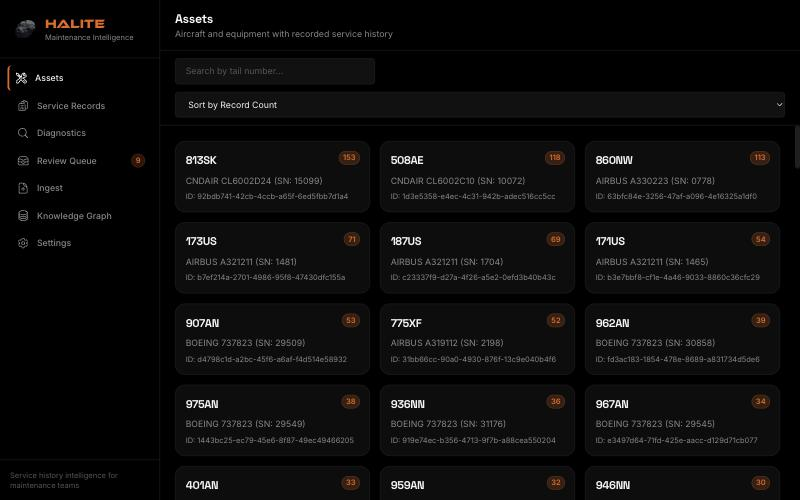
\includegraphics[width=0.92\textwidth]{02_assets_live_corpus.jpg}\caption{Assets: the real corpus with record counts.}\label{fig:shot-assets}\end{figure}
\begin{figure}[H]\centering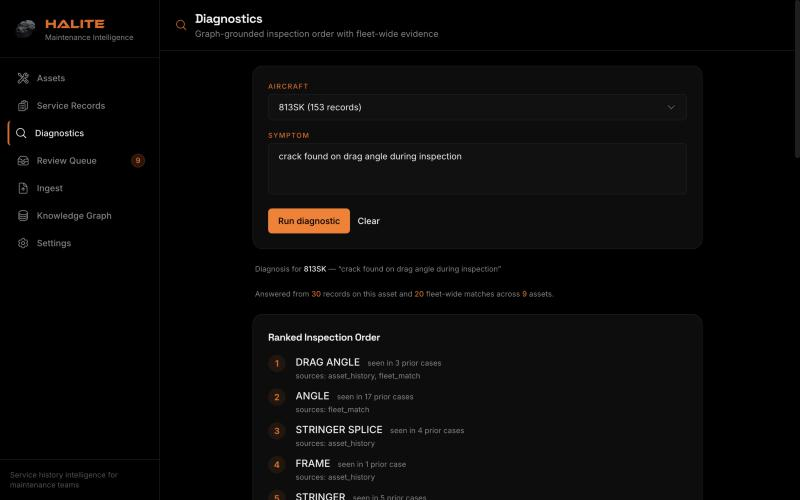
\includegraphics[width=0.92\textwidth]{06_diagnostics_ranked_checks.jpg}\caption{Quick diagnose for aircraft 813SK: ranked inspection order with sources.}\label{fig:shot-diag}\end{figure}
\begin{figure}[H]\centering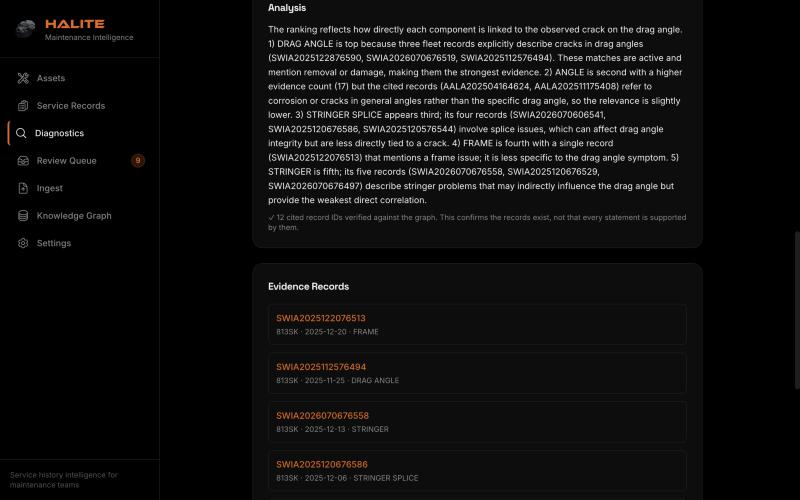
\includegraphics[width=0.92\textwidth]{07_diagnostics_analysis_citations_evidence.jpg}\caption{The model's explanation, the line ``12 cited record IDs verified against the graph'', and the evidence records, each a link.}\label{fig:shot-cite}\end{figure}
\begin{figure}[H]\centering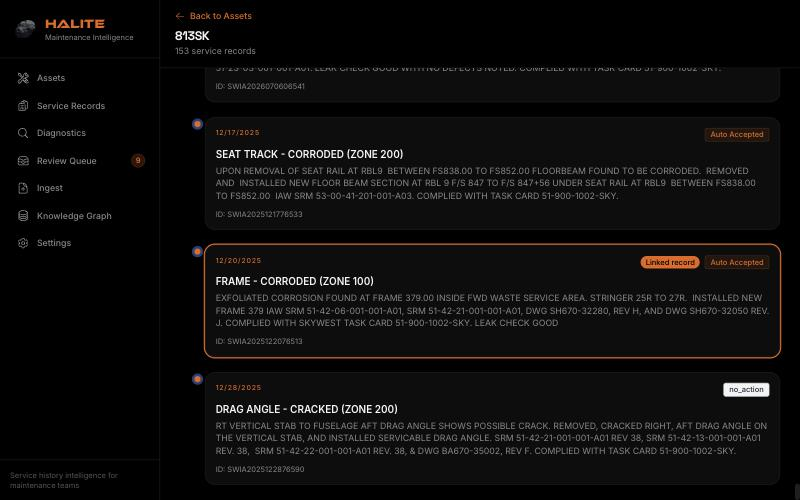
\includegraphics[width=0.92\textwidth]{03_history_linked_record.jpg}\caption{Asset History opened on a cited record, marked as the linked record.}\label{fig:shot-history-linked}\end{figure}
\begin{figure}[H]\centering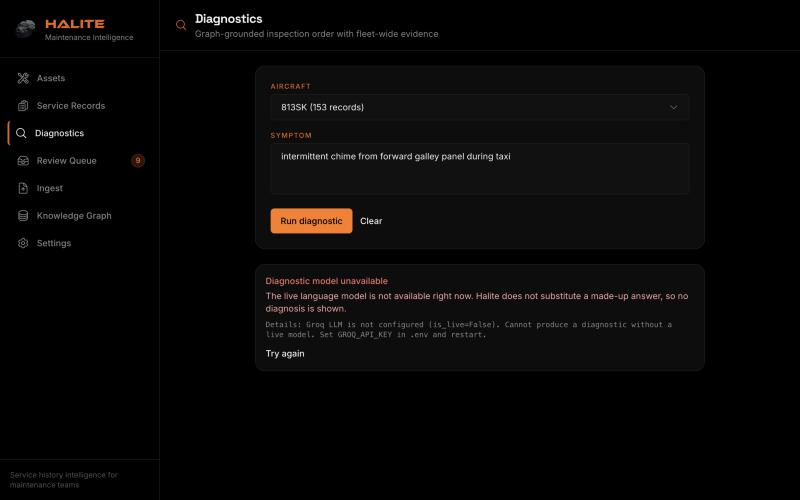
\includegraphics[width=0.92\textwidth]{10_diagnostics_model_unavailable_real_503.jpg}\caption{Failure case: the model is unavailable. The backend's real HTTP 503 reason is shown and no diagnosis is invented.}\label{fig:shot-fail}\end{figure}
\begin{figure}[H]\centering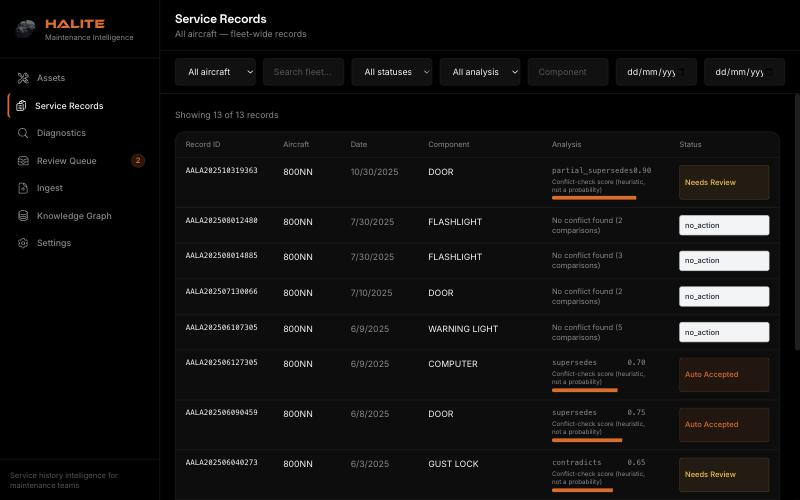
\includegraphics[width=0.92\textwidth]{14_records_scored_800NN.jpg}\caption{Service Records for aircraft 800NN after analysis: label, score (marked heuristic, not a probability) and status per record.}\label{fig:shot-records}\end{figure}
\begin{figure}[H]\centering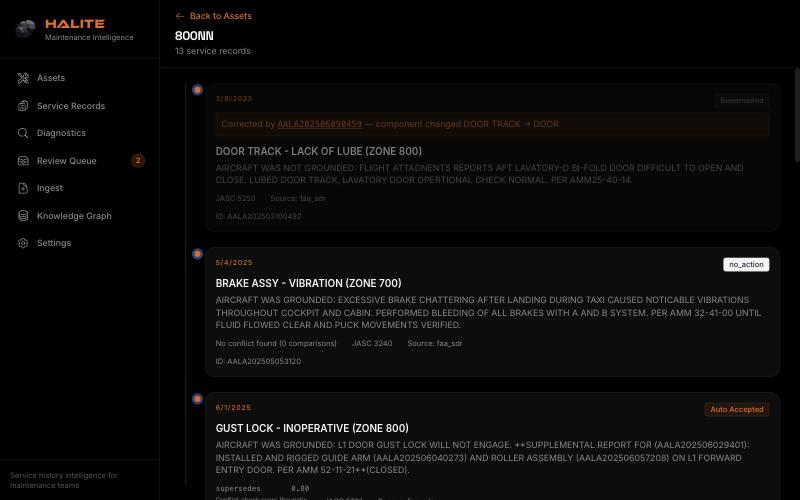
\includegraphics[width=0.92\textwidth]{15_history_correction_800NN.jpg}\caption{Asset History: the older DOOR TRACK record is greyed and reads ``Corrected by \ldots component changed DOOR TRACK $\to$ DOOR''.}\label{fig:shot-history}\end{figure}
\begin{figure}[H]\centering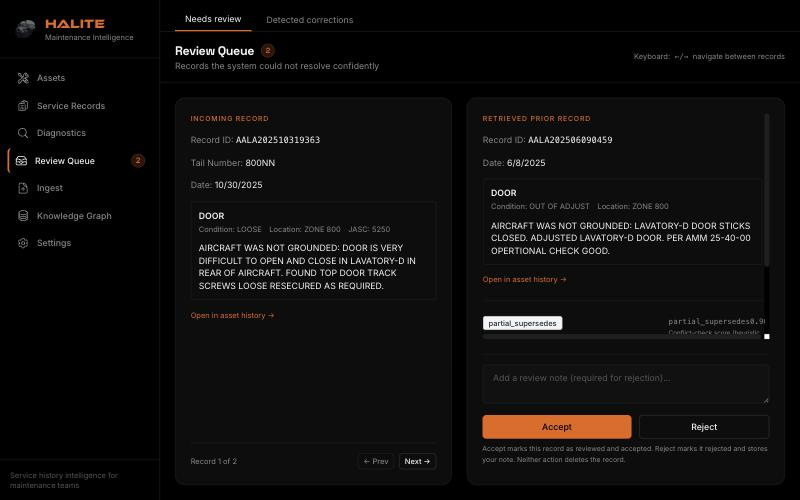
\includegraphics[width=0.92\textwidth]{16_review_queue_800NN.jpg}\caption{Review Queue: the incoming record beside the retrieved prior record, with the model's rationale and the accept and reject actions (not used on this data).}\label{fig:shot-review}\end{figure}
\begin{figure}[H]\centering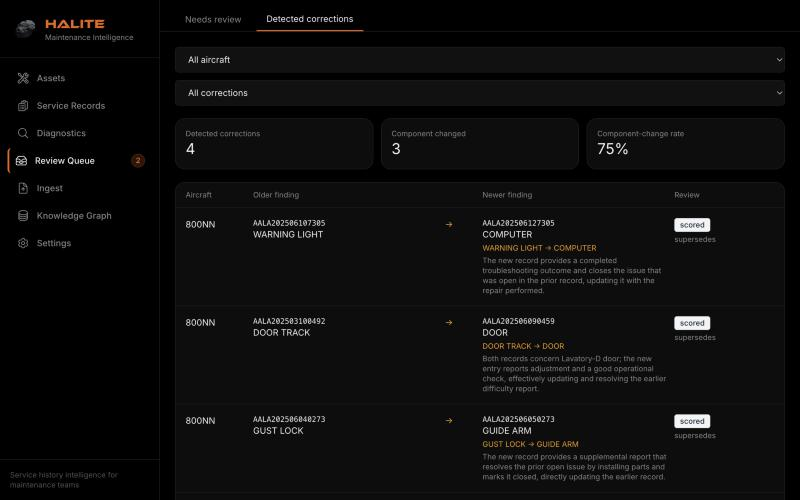
\includegraphics[width=0.92\textwidth]{17_corrections_tab_800NN.jpg}\caption{Detected corrections: four found, three with a component change.}\label{fig:shot-corr}\end{figure}
\begin{figure}[H]\centering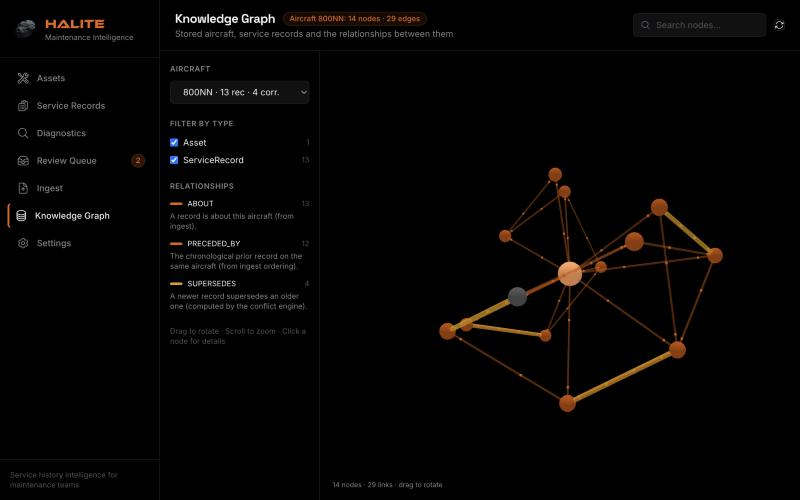
\includegraphics[width=0.92\textwidth]{18_graph_800NN_amber_corrections.jpg}\caption{Knowledge Graph for aircraft 800NN: 14 nodes and 29 edges; the four \code{SUPERSEDES} corrections are thick and amber, the superseded record is grey.}\label{fig:shot-graph}\end{figure}
\begin{figure}[H]\centering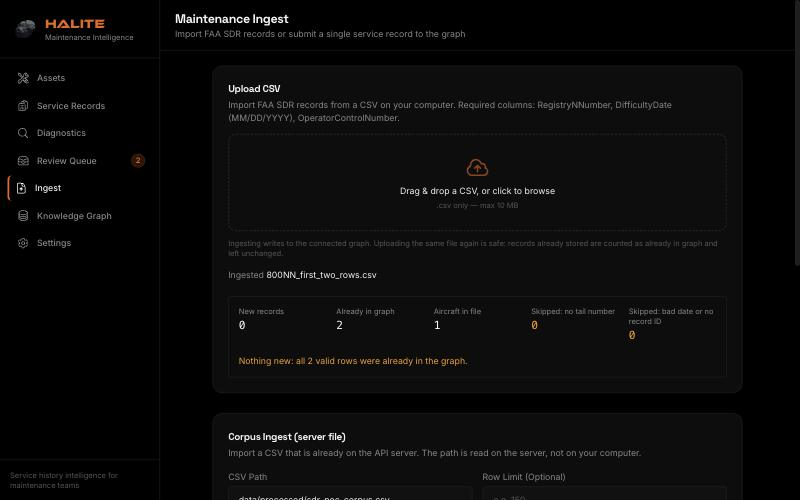
\includegraphics[width=0.92\textwidth]{19_ingest_upload_nothing_new.jpg}\caption{Ingest: re-uploading rows that are already stored reports zero new records and the duplicates, and changes nothing.}\label{fig:shot-ingest}\end{figure}

\section{Iteration Outcome}
Every feature planned for the iteration is implemented at the level stated in Table~\ref{tab:progress}, with three qualifications: retrieval is lexical, the ranking is a heuristic that has not been evaluated against baselines, and the full corpus has not been analysed. The slice runs on real data, is covered by automated tests, and reports its own failures.

\chapter{Testing and Early Validation}\label{ch:testing}

\section{Testing Strategy}
We test at four levels and add manual end-to-end checks against the running system. The aim is that every claim in this report maps to a test, a measurement or a screenshot, and that a failure is reported instead of hidden.
\begin{enumerate}
\item \textbf{Unit tests} of backend services with the language model replaced by a fake, so classification, routing, ranking and citation rules are tested deterministically.
\item \textbf{API tests} that call the routes through FastAPI's test client, including the failure codes (404, 409, 422, 503).
\item \textbf{Repository contract tests} that run the same graph operations against the in-memory store and a real Neo4j service.
\item \textbf{Component tests} of the React pages with the API mocked, covering every response shape and every error state.
\item \textbf{Smoke and end-to-end checks.} A Docker Compose job in CI starts the whole stack and verifies health, the loaded corpus and the maintenance APIs; the acceptance tests T01--T16 are run by hand against a running system.
\end{enumerate}
For the frontend work added late in the iteration we also applied \emph{mutation checks}: after writing a test, we deliberately broke the code it protects (for example, removed a size limit or reverted a label) and confirmed that the test failed, then restored the code.

\section{Test Levels and Techniques}
\begin{longtable}{p{0.34\textwidth}p{0.12\textwidth}p{0.44\textwidth}}
\caption{Automated tests by area (commit \texttt{36a98a3})}\label{tab:testcounts}\\
\toprule \textbf{File} & \textbf{Tests} & \textbf{What it covers} \\ \midrule \endfirsthead
\toprule \textbf{File} & \textbf{Tests} & \textbf{What it covers} \\ \midrule \endhead
\multicolumn{3}{l}{\textit{Backend (PyTest): 194 tests, of which 145 need no database}} \\
\code{test_conflict_engine.py} & 32 & Candidate pairing, classification parsing, adjudication, confidence, routing \\
\code{test_conflict_cascade.py} & 11 & Cost cascade: screen, voting, budget \\
\code{test_api_maintenance.py} & 27 & Maintenance endpoints and failure paths \\
\code{test_diagnostic_retrieval.py} & 26 & Bounded retrieval, ranking, tie-breaks, copilot ranking \\
\code{test_api_copilot.py} & 10 & Copilot contract and failure behaviour \\
\code{test_maintenance_agent.py} & 10 & Ingest: validation, duplicates, orphan repair \\
\code{test_citation_validation.py} & 6 & Identifier extraction and checking \\
\code{test_backfill_conflict_scores.py} & 6 & Resume, budget stop, bounded retries \\
\code{test_api_diagnostics.py}, \code{test_ops.py}, \code{test_conflict_analysis_migration.py} & 4, 3, 3 & Diagnose contract, operations endpoints, legacy-placeholder migration \\
\code{test_regression_software.py} & 7 & Frozen legacy domain still works \\
\code{test_graph_maintenance.py} & 49 & Repository contract against memory and real Neo4j (runs in CI) \\
\midrule
\multicolumn{3}{l}{\textit{Frontend (Vitest): 171 tests in 15 files}} \\
\code{Diagnostics.test.jsx}, \code{DiagnosticsCopilot.test.jsx}, \code{diagnosticsUtils.test.js} & 29, 4, 24 & Diagnose and Copilot states, safety, contract \\
\code{ServiceRecords.test.jsx} & 22 & Fleet list, filters, pagination, deep links \\
\code{ReviewQueue.test.jsx} & 18 & Queue, server-confirmed actions, corrections \\
\code{Graph.test.jsx}, \code{graphScope.test.js} & 18, 10 & Graph selection, counts, edge styling \\
\code{MaintenanceIngest.test.jsx}, \code{ingestClient.test.js} & 17, 1 & CSV upload flow and errors \\
\code{AssetHistory.test.jsx}, \code{Assets.test.jsx} & 12, 3 & History, failure states, list \\
\code{Settings}, \code{Sidebar}, \code{DomainContext}, \code{dummy} & 6, 3, 3, 1 & Navigation and system status \\
\bottomrule
\end{longtable}

\section{Test Cases}
\subsection{End-to-end acceptance tests}
The team defined T01--T16 before the iteration (owner in brackets). Table~\ref{tab:accept} gives each result and its evidence.
\begin{longtable}{p{0.06\textwidth}p{0.27\textwidth}p{0.11\textwidth}p{0.46\textwidth}}
\caption{Acceptance tests and results}\label{tab:accept}\\
\toprule \textbf{ID} & \textbf{Scenario} & \textbf{Result} & \textbf{Evidence and caveat} \\ \midrule \endfirsthead
\toprule \textbf{ID} & \textbf{Scenario} & \textbf{Result} & \textbf{Evidence and caveat} \\ \midrule \endhead
T01 & Application opens the maintenance workspace & Pass & Route smoke log; \code{Sidebar} tests. Browser console was not audited systematically \\
T02 & API lists loaded assets & Pass & \code{test_api_maintenance}; staging lists 118 aircraft \\
T03 & Selected asset history is displayed & Pass & \code{AssetHistory} tests; Figure~\ref{fig:shot-history} \\
T04 & Diagnosis returns graph-backed evidence and ranking & Partly & Full result with a live model locally (Figure~\ref{fig:shot-diag}); on staging fresh diagnoses returned no explanation text on 16 Oct (not re-checked) \\
T05 & Explanation cites a real record that opens & Pass & \code{test_citation_validation}; Figure~\ref{fig:shot-cite}, ``12 cited record IDs verified'' \\
T06 & Unknown asset request & Pass & Controlled 404, ``Aircraft not found'', no invented history \\
T07 & Model unavailable & Pass & HTTP 503 with a reason; Figure~\ref{fig:shot-fail} \\
T08 & Empty or ambiguous evidence & Pass & Explicit ``no relevant history'' result; ranking withheld when there is no evidence \\
T09 & Review queue shows a known case & Pass & Figure~\ref{fig:shot-review} \\
T10 & Review action on a test case & Pass & \code{ReviewQueue} and API tests (confirmation, 409, required note). Accept and reject were \emph{not} exercised live on shared data, on purpose \\
T11 & Frontend tests and build & Pass & 171 tests pass; production build passes \\
T12 & Backend tests & Pass & 194 tests pass in CI \\
T13 & Pull-request CI runs and passes & Pass & Checks run on every pull request; run 39068741787 on \code{36a98a3} succeeded \\
T14 & Real graph health & Pass & Staging reports Neo4j graph mode, live model, 2,079 records (18 Oct); Compose smoke test \\
T15 & Setup on a clean machine & Partly & CI builds the stack from a clean checkout; nobody outside the team has followed the guide \\
T16 & Legacy screen isolation & Pass & \code{Sidebar} and \code{DomainContext} tests; legacy URLs redirect \\
\bottomrule
\end{longtable}
Appendix~\ref{app:tests} lists every automated test by name.

\section{Test Results}
At commit \code{36a98a3} the CI run (id 39068741787) reported: backend \textbf{194 passed}; frontend \textbf{171 passed} in 15 files; the Docker Compose real-graph smoke test passed; the staging deployment that followed succeeded. Code coverage has \textbf{not been measured} (NFR-04), so no coverage figure is claimed.

\section{Acceptance Testing / Validation}
\subsection{One-aircraft analysis run}\label{sec:oneaircraft}
To show scores, corrections and a review queue on real records, and to test the conflict engine on a bounded input, we analysed one aircraft, 800NN (13 records, three FAA-recorded correction pairs), on a throwaway Neo4j graph. Shared staging was not touched. The records were loaded through the new upload route and analysed in the original (\code{legacy}) mode with \code{openai/gpt-oss-120b} and the 0.50 threshold, with an empty classification cache so every result came from a real model call.

\begin{center}
\begin{tabular}{lr}
\toprule \textbf{Measure} & \textbf{Result} \\ \midrule
Records processed & 13 \\
Model classifications / screened without a model & 11 / 2 \\
Successful model requests & 55 \\
Tokens used & 29,386 \\
Rate-limit (HTTP 429) responses, all retried successfully & 27 \\
\code{SUPERSEDES} edges created & 4 \\
Status: no\_action / auto\_accepted / needs\_review & 7 / 4 / 2 \\
FAA-recorded pairs found & \textbf{3 of 3} \\
Edges not in the FAA list & 1 \\
\bottomrule
\end{tabular}
\end{center}
The FAA ground-truth file lists only corrections the FAA reporters themselves recorded, so the one extra edge is \emph{unverified, not shown to be wrong}. We do not compute a precision from one aircraft. Two records were sent to human review. These figures describe this aircraft only: about 2,260 tokens and 4.2 requests per record must not be extrapolated to the full corpus. The method and results are in \pth{docs/mid1/23_single_aircraft_analysis_evidence.md}.

\subsection{Earlier offline evaluation of conflict detection}
An earlier evaluation measured the conflict engine on 350 pairs (141 FAA-recorded positives and 209 sampled negatives, one evaluation per superseding record), with \code{openai/gpt-oss-120b} at threshold 0.50:
\begin{center}
\begin{tabular}{lrrrr}
\toprule \textbf{System} & \textbf{Precision} & \textbf{Recall} & \textbf{F1} & \textbf{False-conflict rate} \\ \midrule
Baseline (most recent prior) & 0.380 & 0.908 & 0.536 & 1.000 \\
Engine (threshold 0.50) & 0.903 & 0.660 & 0.762 & 0.048 \\
\bottomrule
\end{tabular}
\end{center}
The baseline reaches its recall by asserting a supersession on every pair it sees, which is why its false-conflict rate is 1.000. Measured at pair level over the 141 FAA-recorded pairs, precision is 0.788 and recall 0.660; the two precision figures answer different questions and must not be mixed.

\textbf{How far this evidence goes.} It is \emph{historical}: it comes from saved result files of the older run, with a model that is not the one now configured on staging. It measures conflict detection and is \textbf{not} a measure of diagnostic accuracy. The full-corpus counts published with it (121 detected, 117 auto-resolved, 4 for review, 1,617 without candidates) cannot be reproduced from the current code and are not used here.

\section{Edge and Failure Cases}
\begin{longtable}{p{0.3\textwidth}p{0.62\textwidth}}
\caption{Edge and failure cases, and the behaviour tested}\label{tab:edge}\\
\toprule \textbf{Case} & \textbf{Behaviour} \\ \midrule \endfirsthead
\toprule \textbf{Case} & \textbf{Behaviour} \\ \midrule \endhead
Unknown aircraft & 404 and ``Aircraft not found'', never an empty history \\
Aircraft looked up by tail number & The history route takes the UUID; a tail number returns 404 (recorded in the contract) \\
No live model & HTTP 503 with a reason; Copilot returns an empty reply but keeps ranking and evidence \\
Empty model output & Explicit 503, never a blank success \\
Invented record identifier & Marked \code{[UNVERIFIED]} and left out of the valid list \\
Rate limit & Bounded retries; a daily budget stops runs cleanly \\
Superseded record in the Copilot & Visible as evidence, excluded from recommendations \\
Legacy confidence 1.0 & Reported as unscored with null confidence \\
Review action on a record that is not reviewable & HTTP 409; the queue is unchanged \\
Reject without a note & Rejected by validation (HTTP 422) \\
Oversize or non-CSV upload & Rejected in the browser before anything is sent \\
Re-upload of the same CSV & Every record counted as already stored; nothing changes \\
Unreadable CSV (for example empty) & Backend raises an unhandled error (HTTP 500 without CORS headers), which the browser reports as a network failure; the interface words the message to say so (open issue) \\
Browser storage denied or corrupt & Copilot remains usable; a warning is shown \\
\bottomrule
\end{longtable}

\section{Defects and Corrective Actions}
\begin{longtable}{p{0.04\textwidth}p{0.43\textwidth}p{0.4\textwidth}p{0.08\textwidth}}
\caption{Defects found and their resolution}\label{tab:defects}\\
\toprule \textbf{\#} & \textbf{Defect} & \textbf{Corrective action} & \textbf{State} \\ \midrule \endfirsthead
\toprule \textbf{\#} & \textbf{Defect} & \textbf{Corrective action} & \textbf{State} \\ \midrule \endhead
1 & Frontend CI failed: a review-queue test mock lacked \code{getRecord} & Mock fixed; storage shim added for the test environment & Fixed \\
2 & Review-queue ``Open in asset history'' links used tail numbers and led to 404 & Resolve the aircraft UUID; show no link if it cannot be resolved & Fixed \\
3 & Deep link did not scroll when the page was still showing its loading skeleton & Scroll effect depends on the loading state & Fixed \\
4 & Service Records issued 1 + 118 requests on load & Fleet-wide paginated endpoint; two page-initiated calls & Fixed \\
5 & Assets list was slow (one history query per aircraft) & Single aggregation query; about 1.0\,s on staging & Fixed \\
6 & Placeholder confidence 1.0 and ``auto-accepted'' shown as a real result & Honest analysis state; placeholders reported as unscored & Fixed \\
7 & Graph requested 200 nodes yet claimed ``Capped at 2000'' & Request 3,000; truthful counts; warning when the cap is hit & Fixed \\
8 & CSV upload client posted to a route that accepts only a server path; nothing used it & Posts to the upload route; new upload panel & Fixed \\
9 & Small graphs hid their edges behind large nodes & Spacing and node size changed & Fixed \\
10 & Staging fresh diagnoses returned no explanation text & Cause not established (the staging model is smaller); the API reports empty output as 503 & Open \\
11 & Unreadable CSV returns an unhandled HTTP 500 & Interface wording only; backend change belongs to its owner & Open \\
12 & One staging record has no \code{ABOUT} link & Re-running ingest repairs it; not applied to shared data without approval & Open \\
\bottomrule
\end{longtable}

\section{Current Validation Status}
\textbf{Validated:} the code paths covered by 365 automated tests; the end-to-end slice on real records; the failure behaviour in Table~\ref{tab:edge}; the engine on one aircraft against the FAA's own labels (3 of 3). \textbf{Not validated:} diagnostic accuracy of the ranking; retrieval quality against baselines; the engine on the full corpus or with the staging model; usability with real technicians; load performance; code coverage; setup by an outside person. These are planned in Chapter~\ref{ch:remaining}.

\chapter{Project Management and Development Evidence}\label{ch:evidence}

\section{Work Completed}
\begin{itemize}
\item The data pipeline: FAA acquisition, ground-truth extraction, a validated idempotent ingest, 2,079 records on 118 aircraft in Neo4j.
\item The backend: maintenance, diagnostics, graph and operations routes; deterministic retrieval and ranking; citation validation; the conflict engine with an honest analysis state, a budget and an opt-in cost cascade.
\item The frontend: assets, history, fleet records, diagnostics (Copilot and Quick diagnose), review queue and corrections, knowledge graph, CSV ingest, system status.
\item Quality and delivery: 365 automated tests, CI on every push, a CI-gated staging deployment, decision records and a knowledge bank, and dated evidence under \code{docs/mid1/}.
\end{itemize}

\section{Work Remaining}
Hybrid retrieval and its evaluation; role-based access and organisations; server-side session history; the training and analytics modules; analysis of the full corpus; usability testing; coverage measurement; and the open defects in Table~\ref{tab:defects}. Chapter~\ref{ch:remaining} gives the plan.

\section{Individual Responsibilities}
\begin{longtable}{p{0.17\textwidth}p{0.4\textwidth}p{0.33\textwidth}}
\caption{Ownership of files and work packages}\label{tab:owners}\\
\toprule \textbf{Member} & \textbf{Owns} & \textbf{Work packages} \\ \midrule \endfirsthead
\toprule \textbf{Member} & \textbf{Owns} & \textbf{Work packages} \\ \midrule \endhead
Shahmeer Atif (23I-0711) & React pages and components, the Axios client, frontend tests & S1--S5, then the graph view, CSV upload, evidence refresh \\
Muhammad Umar (23I-0782) & Graph schema and queries, diagnose internals, ranking, citation validation, diagnostic tests & U1--U5 \\
Muhammad Usman Al Haq (23I-0585) & Ingest, maintenance APIs, conflict engine, Docker Compose, CI, application wiring & A1--A4, then copilot, confidence and corrections, cost cascade \\
\bottomrule
\end{longtable}

\section{Contribution of Each Team Member}\label{sec:contrib}
Commit and pull-request counts below are evidence of activity, not a measure of contribution; the proposal states the same. They are counted at commit \code{36a98a3}, excluding merge commits. GitHub attributes the commits made under the author name ``Your Name'' (email \code{i230585@isb.nu.edu.pk}) to Usman's account; Shahmeer's commits carry two author identities.
\begin{longtable}{p{0.2\textwidth}p{0.1\textwidth}p{0.22\textwidth}p{0.4\textwidth}}
\caption{Repository activity by member}\label{tab:activity}\\
\toprule \textbf{Member} & \textbf{Commits} & \textbf{Pull requests authored} & \textbf{Main deliverables} \\ \midrule \endfirsthead
\toprule \textbf{Member} & \textbf{Commits} & \textbf{Pull requests authored} & \textbf{Main deliverables} \\ \midrule \endhead
Shahmeer & 20 & \#3, \#4, \#8--\#13 merged; \#14 open & Frontend rework and tests; graph view; CSV upload; knowledge-bank entries for the frontend; evidence documents; this report \\
Umar & 19 & none on GitHub; his branch was merged through the integration branches & Bounded retrieval (U2), deterministic ranking (U3), citation boundary and tests (U4, U5); shared staging deployment workflow and operations API; the knowledge bank and agent protocol \\
Usman & 59 & \#2, \#5, \#6, \#7 merged; \#1 closed unmerged & Maintenance domain and conflict engine, FAA data acquisition and ingest, evaluation harness, maintenance APIs, CI, diagnostic copilot, confidence and corrections, cost cascade \\
\bottomrule
\end{longtable}
\confirm{each member to read their own row and the paragraph below before submission}

\textbf{Shahmeer Atif} rebuilt the maintenance frontend against the frozen backend contract (work packages S1--S5): maintenance-only navigation, asset and history pages with dependable evidence deep links, diagnostics states, a server-confirmed review queue, and the fleet-wide records page that replaced a 119-request fan-out. He then added the one-aircraft knowledge graph, the CSV upload page and the evidence and demonstration documents, and ran and recorded the one-aircraft analysis (Section~\ref{sec:oneaircraft}). \emph{Can demonstrate and explain:} the page code and its tests; the failure model; how each screen reflects a backend field.

\textbf{Muhammad Umar} audited the existing diagnostics (U1), made retrieval bounded on the real Neo4j corpus (U2), wrote the deterministic ranking with a stable tie-break (U3), the citation boundary and its failure behaviour (U4) and the diagnostic backend tests (U5), and set up the shared staging deployment, the operations API and the knowledge bank. \emph{Can demonstrate and explain:} the ranking formula, the retrieval bounds, the citation validation and the staging release path. \confirm{Umar to confirm}

\textbf{Muhammad Usman Al Haq} built the maintenance proof of concept in September (domain registry, FAA acquisition with 141 ground-truth pairs, ingest, the conflict engine and its evaluation) and, in October, the maintenance APIs and hosted CI (A1--A4), then the diagnostic copilot, the honest analysis state with corrections, and the cost cascade. \emph{Can demonstrate and explain:} the conflict pipeline and its routing, the ingest agent, the budget and cascade, and the CI workflows. \confirm{Usman to confirm}

\section{Repository and Version Control Evidence}
The repository is \pth{github.com/umaritics/halite}. Work is organised in feature branches and pull requests; each pull request ran the CI checks before merge. Table~\ref{tab:prs} lists them.
\begin{longtable}{p{0.06\textwidth}p{0.2\textwidth}p{0.12\textwidth}p{0.5\textwidth}}
\caption{Pull requests}\label{tab:prs}\\
\toprule \textbf{PR} & \textbf{Author} & \textbf{State} & \textbf{Title} \\ \midrule \endfirsthead
\toprule \textbf{PR} & \textbf{Author} & \textbf{State} & \textbf{Title} \\ \midrule \endhead
\#1 & Usman & closed & Maintenance domain integration (September proof of concept; the commits are in \code{main}'s history through the integration branch) \\
\#2 & Usman & merged & Mid-I backend release hygiene closure \\
\#3 & Shahmeer & merged & Frontend maintenance UX, Service Records performance, diagnose and review hardening \\
\#4 & Shahmeer & merged & Frontend reflects backend outputs \\
\#5 & Usman & merged & Evidence-grounded diagnostic copilot \\
\#6 & Usman & merged & Confidence, corrections, conflict-cost evidence \\
\#7 & Usman & merged & Opt-in conflict-analysis cost cascade \\
\#8 & Shahmeer & merged & Documentation sync after \#5--\#7 \\
\#9 & Shahmeer & merged & Knowledge graph focused on one aircraft \\
\#10 & Shahmeer & merged & CSV upload with honest counts and inline errors \\
\#11 & Shahmeer & merged & Graph spacing and layout settling \\
\#12 & Shahmeer & merged & Single-aircraft analysis evidence \\
\#13 & Shahmeer & merged & Frontend evidence and demo script refresh \\
\#14 & Shahmeer & open & WebGL check and error boundary for the graph \\
\bottomrule
\end{longtable}
\textbf{Release marking.} \confirm{release tag name and the commit it marks; not yet created at the time of writing}

\section{Milestones and Commit Evidence}
\begin{longtable}{p{0.16\textwidth}p{0.45\textwidth}p{0.3\textwidth}}
\caption{Milestone log with evidence}\label{tab:milestones}\\
\toprule \textbf{Date (2026)} & \textbf{Milestone} & \textbf{Evidence} \\ \midrule \endfirsthead
\toprule \textbf{Date (2026)} & \textbf{Milestone} & \textbf{Evidence} \\ \midrule \endhead
11 Jul -- 18 Aug & Earlier software-engineering prototype (later set aside) & Commits by Umar's account \\
8 -- 10 Sep & Maintenance proof of concept: domain registry, FAA acquisition, conflict engine, evaluation harness, first maintenance screens & Commits T0--T10, C--E, F, G, H, J \\
15 Oct & Mid-I engineering blueprint; runtime smoke test fixed in CI & \pth{docs/halite_work_division_mid1.pdf}; commit \code{2651eab} \\
16 Oct & Frontend S1--S5; retrieval, ranking and citation boundary U2--U5; staging deployment; PRs \#2--\#5 merged & Commits; \code{docs/mid1/02}, \code{08}, \code{11}--\code{13} \\
17 Oct & Confidence and corrections; cost cascade; knowledge graph; PRs \#6, \#7, \#9 & \code{docs/mid1/19}--\code{21} \\
18 Oct & CSV upload; evidence refresh; one-aircraft analysis; this report; PRs \#10--\#13 & \code{docs/mid1/23}; CI run 39068741787 \\
\bottomrule
\end{longtable}

\section{Tools and Tool-Assisted Development}\label{sec:tools}
\textbf{Disclosure.} The team used three generative-AI tools during development and during the preparation of this report: \textbf{Claude} (Claude Code, model Claude Sonnet 5.5), \textbf{OpenAI Codex} and \textbf{Cursor}. This section states what is recorded about each, how the output was checked, and where each member must add to it. The proposal committed the team to an AI usage log (\S3.9.4); the repository's agent protocol (\code{AGENTS.md}) and the existing report addendum (\code{docs/mid1/15}) already say that a tool's absence from a list is not permission to omit it.

\begin{longtable}{p{0.14\textwidth}p{0.36\textwidth}p{0.4\textwidth}}
\caption{Generative-AI tools used}\label{tab:aitools}\\
\toprule \textbf{Tool} & \textbf{Where it is recorded in the repository} & \textbf{Recorded use} \\ \midrule \endfirsthead
\toprule \textbf{Tool} & \textbf{Where it is recorded} & \textbf{Recorded use} \\ \midrule \endhead
Claude Code (Claude Sonnet 5.5) & \code{Co-Authored-By} trailers on the commits it helped write; the frontend, knowledge-bank and evidence documents & Frontend code and tests (work packages S1--S5 and PRs \#3, \#4, \#8--\#14), knowledge-bank and evidence documents, the one-aircraft analysis run, and the drafting of this report from the repository and its evidence \\
OpenAI Codex & \pth{docs/mid1/15_report_mid1_addendum.md} & The 16 October integration audit: inspecting repository state, proposing scoped edits, running tests and builds, drafting engineering documentation \\
Cursor & \code{Co-authored-by: Cursor} trailers on five commits (four on 11 July, one on 15 October); \code{.cursor/rules}; \pth{docs/mid1/22_cursor_handoff_2026-10-17.md} & Backend work and hand-offs recorded in the repository; \confirm{Umar and Usman to state which work packages used Cursor and for what} \\
\bottomrule
\end{longtable}

\textbf{Member statements.}
\begin{longtable}{p{0.16\textwidth}p{0.18\textwidth}p{0.62\textwidth}}
\toprule \textbf{Member} & \textbf{Tools} & \textbf{Used for, and what the member verified} \\ \midrule \endhead
Shahmeer & Claude Code & Frontend and documentation. Verified every change by running the tests and the build, by mutation checks on new tests, by live checks in a browser against a running backend, and by reading each diff before merging \\
Umar & \confirm{tools} & \confirm{purpose and verification} \\
Usman & \confirm{tools} & \confirm{purpose and verification} \\
\bottomrule
\end{longtable}

\textbf{Checks applied to tool output.} Code produced with a tool was accepted only after (1) the automated tests and the build passed, (2) for new tests, a mutation check showed that the test fails when the protected code is broken, (3) the behaviour was checked live where a running system was available, (4) another member could review it through a pull request with CI, and (5) numbers in documents were traced to a test, a measurement or a CI log. Where something could not be verified, the documents say so. The members remain responsible for being able to explain every change.

\textbf{Not a development tool.} The Groq-hosted language model is an external component of the product, not a development assistant; it is described in Section~\ref{sec:external}.

\section{External Components and Dependencies}
The runtime and development dependencies are in Table~\ref{tab:tools}. The data source is the FAA Service Difficulty Report collection \citep{faa-sdr}, public domain, downloaded by script and excluded from version control. The language model is called over the network, is rate limited, and can be replaced without changing the ranking, the graph or the citation check.

\section{Risks and Mitigation}\label{sec:risks}
\begin{longtable}{p{0.06\textwidth}p{0.28\textwidth}p{0.5\textwidth}p{0.08\textwidth}}
\caption{Risk register and outcome}\label{tab:risks}\\
\toprule \textbf{ID} & \textbf{Risk} & \textbf{Mitigation and what happened} & \textbf{State} \\ \midrule \endfirsthead
\toprule \textbf{ID} & \textbf{Risk} & \textbf{Mitigation and what happened} & \textbf{State} \\ \midrule \endhead
R1 & Too much new code in too little time & Occurred in part: 77 commits in four days. Mitigation: ownership, small pull requests, CI, tests, decision records; each member explains their own code & Residual \\
R2 & Graph unavailable & Compose smoke test; health endpoint reports the real mode & Mitigated \\
R3 & Live model or key unavailable & 503 and failure screens; occurred on staging (empty explanations) & Open \\
R4 & Different JSON assumptions between owners & Contract freeze and recorded fixtures; one miss (UUID versus tail number) fixed & Mitigated \\
R5 & Merge conflicts from several people and tools & One owner per file, hand-off decisions, small pull requests & Mitigated \\
R6 & Exposed secrets & Secrets only in ignored files; audit by Usman; \code{.env.local} was found not to be in \code{.gitignore} and must not be committed & Residual \\
R7 & Wrong dataset version & Dataset profile and counts recorded with the file year & Mitigated \\
R8 & No hosted CI proof & CI on \code{main}; run 39068741787 & Mitigated \\
R9 & Legacy software scope leaks into the interface & Isolation by routing; tests & Mitigated \\
R10 & Conflict metrics presented as diagnostic accuracy & Addendum and this report keep them apart & Mitigated \\
R11 & Missing university artefacts & This report; evidence documents & Mitigated \\
R12 & Shared staging data changed by a demonstration & Staging is read-only for demonstrations; analysis was run on a scratch graph & Mitigated \\
R13 & Model quota and cost & Daily budget, bounded retries, opt-in cascade; full run deferred & Residual \\
R14 & Unauthenticated destructive endpoint (\pth{DELETE /api/graph/reset}) & Removed from the interface; the route itself remains & Open \\
\bottomrule
\end{longtable}

\section{Security and Privacy Considerations}
No personal data about users is stored; the corpus holds public FAA reports. Secrets (model key, database password, operations token, deployment keys) are read from environment files that are not committed. The batch analysis endpoint and the log endpoint require an operations token. Authentication and authorisation for ordinary users do not exist yet. The graph-reset route is the known gap in Table~\ref{tab:risks}. Staging is shared, so the team avoids writing to it for demonstrations.

\section{Current Limitations}
\begin{itemize}
\item The ranking is a heuristic with unevaluated weights; semantic retrieval is not built.
\item The full corpus has not been analysed; on staging every record is unanalysed.
\item No authentication, organisations or reviewer identity; the audit trail records status and a note, not who acted.
\item Copilot sessions live in the browser only.
\item No usability study, load test or coverage measurement.
\item The staging model differs from the model used for the evaluation; staging explanations were empty on 16 October.
\item The graph side panel was verified by unit tests, not by a live click.
\end{itemize}

\chapter{Remaining FYP Plan}\label{ch:remaining}

\section{Remaining Scope}
The proposal's nine modules and thirteen objectives remain the scope of the project. At this mid-report four modules are in a working vertical slice (Table~\ref{tab:scope}); the rest, and the evaluation that makes the research claims, remain. Nothing is dropped. The plan below is ordered by what the research questions need first: a measured retrieval baseline, then the evaluation of correction-aware ranking, then the product features around them.

\section{Remaining Modules and Features}
\begin{longtable}{p{0.2\textwidth}p{0.26\textwidth}p{0.44\textwidth}}
\caption{Remaining work by module}\label{tab:remmods}\\
\toprule \textbf{Module} & \textbf{State now} & \textbf{Remaining} \\ \midrule \endfirsthead
\toprule \textbf{Module} & \textbf{State now} & \textbf{Remaining} \\ \midrule \endhead
M01 Workspace & Not started & Authentication, roles, organisations, reviewer identity in the audit trail \\
M02 Assets & Working & Manual asset registration; component view \\
M03 Knowledge graph & Working (one aircraft) & Component-level graph; path exploration; fallback when WebGL is missing (pull request open) \\
M04 Diagnostics & Working (lexical, heuristic) & Semantic and hybrid retrieval; evaluation against baselines; server-side session history; clarification policy \\
M05 Conflict intelligence & Working; mostly unanalysed & Token measurement; full-corpus analysis with the cascade; review audit log \\
M06 Report intelligence & CSV and single record & Extraction from documents; ambiguous-field flags \\
M07 Academy & Not started & Case-based scenarios, learner steps, feedback linked to evidence \\
M08 Analytics & Not started & Recurring-fault and fleet views with descriptive statistics only \\
M09 Administration & Status page only & Audit, configuration, governance \\
\bottomrule
\end{longtable}

\section{Remaining Iterations}
The proposal's later iterations stand: \textbf{Iteration 2 (FYP-1 Final)}, an integrated minimum viable product with hybrid retrieval, role-based access, multi-turn sessions with server-side history and a deployed demonstration; \textbf{Iteration 3 (FYP-2 Early)} for training, analytics and graph exploration; \textbf{Iteration 4 (FYP-2 Mid)}, a job-fair-ready integrated product; and \textbf{Iteration 5 (FYP-2 Final)} for hardening, final evaluation and handover. The percentages in the timeline are targets, not measured progress.

\section{Implementation Plan}
\textbf{Iteration 2 (FYP-1 Final).} Tasks are ordered by dependency; owners follow the ownership in Table~\ref{tab:owners}.
\begin{longtable}{p{0.05\textwidth}p{0.5\textwidth}p{0.14\textwidth}p{0.21\textwidth}}
\toprule \textbf{\#} & \textbf{Task} & \textbf{Owner} & \textbf{Done when} \\ \midrule \endhead
1 & Close the open defects in Table~\ref{tab:defects}: staging explanations, an HTTP 400 for unreadable CSV, the orphan record, protection of the graph-reset route & Usman, Umar & Each has a test or a recorded check \\
2 & Measure live token use on a bounded sample and project the full-corpus cost; decide the default analysis mode & Usman & Measured numbers in an evidence document \\
3 & Embedding-based retrieval and a hybrid ranker behind a switch & Umar & Runs on the corpus; unit tests \\
4 & Diagnostic evaluation harness and baselines (keyword, lexical, semantic, graph-only, hybrid, direct model) & Umar, Usman & Metrics reproducible from a script \\
5 & Roles and authentication; reviewer identity in the audit trail & Usman, Shahmeer & Requests carry an identity; review events record who and when \\
6 & Server-side session history for the Copilot & Umar, Shahmeer & Sessions survive a browser change \\
7 & Analysis of the full corpus with the cascade on a scratch graph, then staging with approval & Usman & Coverage shown in the interface \\
8 & Quality: lint job in CI, coverage report for core modules, release tags & Shahmeer, Usman & CI reports them \\
\bottomrule
\end{longtable}

\section{Testing and Validation Plan}
\begin{longtable}{p{0.07\textwidth}p{0.4\textwidth}p{0.43\textwidth}}
\caption{Validation plan against the research questions}\label{tab:valplan}\\
\toprule \textbf{RQ} & \textbf{Question} & \textbf{Planned evidence} \\ \midrule \endfirsthead
\toprule \textbf{RQ} & \textbf{Question} & \textbf{Planned evidence} \\ \midrule \endhead
RQ1 & Does graph-constrained retrieval beat keyword retrieval at finding relevant cases? & Recall at $k$ and mean reciprocal rank on the 141 FAA pairs, same queries for both methods \\
RQ2 & Does hybrid retrieval improve ranking over semantic alone? & Same metrics, with an ablation of each signal \\
RQ3 & Does correction-aware retrieval reduce misleading recommendations? & Using the FAA pairs in which the follow-up names a different component (92 of 141): does the system surface the later component for the earlier symptom? \\
RQ4 & Can abstention reduce unsupported suggestions? & Coverage against error rate as the evidence threshold changes \\
RQ5 & Does case-based training improve learners' results? & Planned with the training module in FYP-2 \\
\bottomrule
\end{longtable}
To avoid leakage the evaluation will use a different year of FAA data than the one used to choose weights and thresholds, and any threshold will be fixed before it is applied to held-out data, as the cascade threshold was. Usability will be measured with proxy participants (a task and a System Usability Scale questionnaire), which the proposal already says will be declared as proxies. Load performance will be tested against the 500~ms target (NFR-02), and coverage measured against NFR-04.

\section{Deployment Plan}
The staging deployment, with its recorded rollback and approval gate, is the model for later releases. For FYP-2 the plan is a production-style deployment of the same pipeline with backups of the graph before any migration, read-only demonstrations on shared data, and a prerecorded backup of every demonstration.

\section{Tentative Timeline}
Dates follow the university calendar once it is published; the weeks below are relative to the FYP-1 Final evaluation.
\begin{longtable}{p{0.18\textwidth}p{0.72\textwidth}}
\toprule \textbf{Period} & \textbf{Work} \\ \midrule \endhead
Weeks 1--2 & Close open defects (task 1); live token measurement (task 2); lint and coverage in CI (task 8) \\
Weeks 3--5 & Embedding retrieval and hybrid ranker (task 3); evaluation harness and baselines (task 4) \\
Weeks 4--6 & Roles, authentication and reviewer identity (task 5) \\
Weeks 6--7 & Server-side session history (task 6); full-corpus analysis on a scratch graph (task 7) \\
Week 8 & Integration, regression, updated requirements and design specification, rehearsal \\
\bottomrule
\end{longtable}
Each week ends with a demonstrable milestone, recorded with its evidence in the milestone log, so that progress is checkable against the demonstration and not against a task list.

\section{Expected Final Deliverables}
A deployed, tested and documented multi-user system with the nine modules; a reproducible evaluation against baselines with stated limits; the repository with tags, setup instructions and decision records; the final report; and a demonstration that every member can explain.

\chapter{Conclusion}\label{ch:conclusion}
Maintenance records are evidence that changes over time: a later report can correct an earlier one, often by naming a different component. In the FAA reports we studied, 65.2\% of the correction pairs the reporters wrote themselves point to a different part. Halite is built around that fact. It stores records and their order in a graph, links a correction to the record it replaces, retrieves evidence from a bounded neighbourhood of that graph, ranks components with a documented deterministic heuristic, checks every cited record identifier against the data, and sends records it cannot resolve to a human.

At FYP-1 Mid the project has a working vertical slice on 2,079 real records for 118 aircraft: asset history, a one-aircraft knowledge graph, a multi-turn diagnostic assistant, a conflict engine with a review queue, a CSV upload path, 371 automated tests that pass in continuous integration, a deployment pipeline gated by those tests, and a live re-validation that found, and then fixed, a defect the tests could not see. On one aircraft the conflict engine found all three corrections the FAA itself recorded.

The report is equally clear about what is not yet shown. The ranking is a heuristic whose weights have not been evaluated; semantic retrieval is not built; most of the corpus has not been analysed; there is no authentication; and the earlier evaluation of conflict detection is historical and says nothing about diagnostic accuracy. Most of the code was merged in the last days before this report, so we have tied every module to a named owner, a test and a decision record, and every member must be able to explain their part.

FYP-1 Final starts with a measured baseline and the closing of the open defects, then adds hybrid retrieval, an evaluation against baselines, role-based access and server-side sessions. FYP-2 adds the training and analytics modules and the final evaluation. The research contribution---correction-aware retrieval that preserves provenance and abstains when evidence is weak---will be judged by that evaluation, not by this report.


\appendix
\chapter{Proposal Action Register}\label{app:register}
\section*{Panel actions}
No panel feedback or required changes were issued at the proposal stage, so no panel action exists to register. The supervisor can confirm this.

\section*{Corrections the team made to its own proposal}
\begin{longtable}{p{0.05\textwidth}p{0.24\textwidth}p{0.33\textwidth}p{0.1\textwidth}p{0.18\textwidth}}
\toprule \textbf{No.} & \textbf{Statement in the proposal} & \textbf{Correction} & \textbf{Status} & \textbf{Evidence} \\ \midrule \endhead
T1 & Embedding-based and hybrid retrieval are described in the proposal's \S10.4 & Stated as planned for FYP-1 Final; implemented retrieval is lexical over a bounded candidate set & Corrected & \texttt{docs/mid1/15\_report\_mid1\_addendum.md}; Table~\ref{tab:compare} \\
T2 & About 60 airframes & 118 aircraft, because every aircraft with a ground-truth pair is selected first & Corrected & \texttt{docs/dataset\_profile.md}; Section~\ref{sec:data} \\
T3 & A complete nine-module product at Mid & A vertical slice through four modules, with every module's scope stated & Corrected & Table~\ref{tab:scope} \\
\bottomrule
\end{longtable}

\chapter{Detailed Requirements}\label{app:req}
The requirement identifiers are those of the proposal. The status is the status at this mid-report: Met, Partial, Deferred (outside the Mid scope), or Not measured.

\section*{Functional requirements}
\begin{longtable}{p{0.09\textwidth}p{0.36\textwidth}p{0.14\textwidth}p{0.31\textwidth}}
\caption{All functional requirements and their Mid status}\label{tab:allfr}\\
\toprule \textbf{ID} & \textbf{Requirement} & \textbf{Mid status} & \textbf{Evidence or reason} \\ \midrule \endfirsthead
\toprule \textbf{ID} & \textbf{Requirement} & \textbf{Mid status} & \textbf{Evidence or reason} \\ \midrule \endhead
FR-01 & Authenticate authorised users & Deferred & No authentication yet \\
FR-02 & Associate users with organisations & Deferred & No organisations yet \\
FR-03 & Enforce role-based permissions & Deferred & FYP-1 Final \\
FR-04 & Prevent cross-tenant access & Deferred & No tenancy \\
FR-05 & Register maintenance assets & Partial & Assets are created by ingest; no registration screen \\
FR-06 & Show chronological records for an asset & Met & \code{AssetHistory.test} (12); API 404 for unknown asset \\
FR-07 & Search assets by identifier & Met & \code{Assets.test} \\
FR-08 & Show record-linked diagnostic and conflict information & Met & Corrected-by banner; \code{ServiceRecords.test} (22) \\
FR-09 & Accept supported report formats & Partial & FAA CSV by upload or path; single record; no PDF or DOCX for maintenance \\
FR-10 & Extract asset, component, symptom and date & Partial & Structured CSV fields only; no free-text extraction \\
FR-11 & Retain the original source record & Met & Text and identifier stored; reject never deletes \\
FR-12 & Flag ambiguous extraction fields & Partial & Skipped rows counted by reason; no per-field flags \\
FR-13 & Create relationships among entities & Met & \code{test_maintenance_agent} (10) \\
FR-14 & Traverse related historical cases & Met & \code{Graph.test}, \code{graphScope.test} \\
FR-15 & Expose provenance of graph results & Met & Edge legend; record \code{source} \\
FR-16 & Accept natural-language symptoms & Met & \code{test_api_diagnostics}, \code{test_api_copilot} \\
FR-17 & Retrieve relevant historical evidence & Met (lexical) & \code{test_diagnostic_retrieval} (26) \\
FR-18 & Rank hypotheses when evidence suffices & Met (heuristic) & Deterministic ranking tests \\
FR-19 & Display supporting record references & Met & Evidence links; \code{Diagnostics.test} (29) \\
FR-20 & Request clarification when information is missing & Partial & Copilot asks at most one question \\
FR-21 & Distinguish unsupported from verified & Met & \code{test_citation_validation} (6) \\
FR-22 & Preserve diagnostic session history & Partial & Browser storage only \\
FR-23 & Compare new records with prior records & Met & \code{test_conflict_engine} (32) \\
FR-24 & Classify potential conflicts & Met & Five labels; parse-failure routing \\
FR-25 & Route uncertain cases for review & Met & Routing tests; threshold 0.50 \\
FR-26 & Record supervisor review decisions & Met & No reviewer identity \\
FR-27 & Audit trail of status changes & Partial & Status and note stored; no actor or event log \\
FR-28 & Start a training case & Deferred & FYP-2 \\
FR-29 & Record learner steps & Deferred & FYP-2 \\
FR-30 & Feedback linked to case evidence & Deferred & FYP-2 \\
FR-31 & Store training completion history & Deferred & FYP-2 \\
FR-32 & Display recorded fault trends & Deferred & FYP-2 \\
FR-33 & Identify repeated faults on the same asset & Deferred & FYP-2 \\
FR-34 & Filters by asset, component and date range & Partial & Service Records filters exist; no analytics view \\
FR-35 & Distinguish descriptive statistics from predictions & Deferred & FYP-2 \\
\bottomrule
\end{longtable}

\section*{Non-functional requirements}
\begin{longtable}{p{0.09\textwidth}p{0.36\textwidth}p{0.14\textwidth}p{0.31\textwidth}}
\caption{All non-functional requirements and their Mid status}\label{tab:allnfr}\\
\toprule \textbf{ID} & \textbf{Requirement} & \textbf{Mid status} & \textbf{Evidence or reason} \\ \midrule \endfirsthead
\toprule \textbf{ID} & \textbf{Requirement} & \textbf{Mid status} & \textbf{Evidence or reason} \\ \midrule \endhead
NFR-01 & Availability & Partial & Staging reachable at each check; no uptime monitoring \\
NFR-02 & API performance, p95 $\le$ 500 ms & Not shown to be met & One observed 0.99 s request exceeds 500 ms; a p95 cannot be established from one measurement; no load test \\
NFR-03 & Diagnostic latency measured & Not measured & Fresh diagnoses call an external model \\
NFR-04 & 80\% coverage of core backend modules & Not measured & No coverage run; test counts only \\
NFR-05 & No unauthorised tenant access & Deferred & No tenancy yet \\
NFR-06 & Failed external operations reported and retried safely & Met & Bounded retries; 503; failure states \\
NFR-07 & Citations resolve to real record IDs & Met & Citation validation and tests \\
NFR-08 & Usability measured & Not measured & No user study \\
NFR-09 & Independent setup succeeds & Partial & Setup guide and CI Compose smoke; no outside run \\
NFR-10 & Review changes traceable to actor and time & Partial & No actor recorded \\
\bottomrule
\end{longtable}

\section*{Summary of functional requirements}
Of the 35 functional requirements: deferred 11, met 16, partial 8.

\chapter{Detailed Test Cases}\label{app:tests}
These lists are generated from the test runners by \texttt{gen\_appendix\_tests.py}; they are not typed by hand. Test names describe the behaviour checked. The Neo4j repository-contract file is collected here and executed only in CI, against a real Neo4j service.
\section{Backend tests (194 tests)}\label{app:tests-backend}
\small
\subsection*{\texttt{test\_api\_copilot.py} (10)}
\begin{longtable}{p{0.05\textwidth}p{0.9\textwidth}}
1 & test\_second\_turn\_reranks\_accumulated\_case\_and\_reports\_delta \\
2 & test\_ruled\_out\_component\_is\_not\_recommended \\
3 & test\_invalid\_citation\_is\_flagged\_and\_never\_verified \\
4 & test\_superseded\_record\_is\_marked\_but\_not\_used\_in\_ranked\_recommendations \\
5 & test\_validation\_unknown\_asset\_and\_model\_failure\_states \\
6 & test\_fleet\_only\_mode\_and\_deterministic\_record\_report\_selection \\
7 & test\_period\_and\_topic\_report\_selects\_only\_matching\_asset\_records \\
8 & test\_diagnose\_empty\_explanation\_regression\_is\_explicit\_503 \\
9 & test\_groq\_wrapper\_rejects\_none\_content\_with\_finish\_reason \\
10 & test\_groq\_wrapper\_returns\_provider\_usage\_metadata \\
\end{longtable}
\subsection*{\texttt{test\_api\_diagnostics.py} (4)}
\begin{longtable}{p{0.05\textwidth}p{0.9\textwidth}}
1 & TestDiagnoseLlmBoundary > test\_503\_when\_llm\_not\_live \\
2 & TestDiagnoseLlmBoundary > test\_404\_when\_no\_history \\
3 & TestDiagnoseCitations > test\_flags\_invented\_ids\_keeps\_real \\
4 & TestDiagnoseCitations > test\_all\_valid\_when\_only\_graph\_ids \\
\end{longtable}
\subsection*{\texttt{test\_api\_maintenance.py} (27)}
\begin{longtable}{p{0.05\textwidth}p{0.9\textwidth}}
1 & TestDomains > test\_returns\_two\_domains \\
2 & TestDomains > test\_software\_is\_default \\
3 & TestDomains > test\_maintenance\_not\_default \\
4 & TestDomains > test\_domain\_has\_required\_fields \\
5 & TestHealthMaintenance > test\_health\_includes\_domains \\
6 & TestHealthMaintenance > test\_health\_includes\_maintenance\_fields \\
7 & TestHealthMaintenance > test\_health\_maintenance\_false\_before\_ingest \\
8 & TestHealthMaintenance > test\_health\_uses\_count\_query\_not\_record\_materialization \\
9 & TestAssetsEmpty > test\_returns\_empty\_list \\
10 & TestAssetsEmpty > test\_unknown\_asset\_history\_is\_404 \\
11 & TestAssetsEmpty > test\_ingest\_rejects\_non\_positive\_limit \\
12 & TestAssetsEmpty > test\_record\_processing\_rejects\_invalid\_threshold \\
13 & TestIngestAndQuery > test\_assets\_listed\_after\_seed \\
14 & TestIngestAndQuery > test\_asset\_history\_returned \\
15 & TestIngestAndQuery > test\_legacy\_perfect\_score\_is\_returned\_as\_not\_analysed \\
16 & TestIngestAndQuery > test\_review\_queue\_returns\_needs\_review \\
17 & TestIngestAndQuery > test\_accept\_changes\_status \\
18 & TestIngestAndQuery > test\_reject\_requires\_note \\
19 & TestIngestAndQuery > test\_reject\_disallows\_blank\_note \\
20 & TestIngestAndQuery > test\_reject\_with\_note\_succeeds \\
21 & TestIngestAndQuery > test\_reject\_cannot\_overwrite\_completed\_review \\
22 & TestIngestAndQuery > test\_conflict\_detection\_on\_seeded\_record \\
23 & TestConflictAnalysisApi > test\_status\_counts\_and\_records\_list\_limit\_validation \\
24 & TestConflictAnalysisApi > test\_analysis\_run\_requires\_token\_and\_live\_llm \\
25 & TestConflictAnalysisApi > test\_no\_candidate\_is\_analysed\_without\_model\_call\_and\_scored\_is\_skipped \\
26 & TestConflictAnalysisApi > test\_analysis\_run\_stops\_cleanly\_at\_persistent\_budget \\
27 & TestConflictAnalysisApi > test\_corrections\_endpoint\_returns\_live\_summary \\
\end{longtable}
\subsection*{\texttt{test\_backfill\_conflict\_scores.py} (6)}
\begin{longtable}{p{0.05\textwidth}p{0.9\textwidth}}
1 & test\_backfill\_refuses\_to\_run\_without\_live\_groq \\
2 & test\_resume\_uses\_analysis\_state\_only[record0-True] \\
3 & test\_resume\_uses\_analysis\_state\_only[record1-False] \\
4 & test\_resume\_uses\_analysis\_state\_only[record2-False] \\
5 & test\_resume\_uses\_analysis\_state\_only[record3-False] \\
6 & test\_resume\_uses\_analysis\_state\_only[record4-True] \\
\end{longtable}
\subsection*{\texttt{test\_citation\_validation.py} (6)}
\begin{longtable}{p{0.05\textwidth}p{0.9\textwidth}}
1 & TestExtractRecordIdCandidates > test\_real\_faa\_shapes \\
2 & TestExtractRecordIdCandidates > test\_dedupes\_preserving\_order \\
3 & TestExtractRecordIdCandidates > test\_ignores\_short\_or\_underscore\_ids \\
4 & TestValidateCitations > test\_all\_valid \\
5 & TestValidateCitations > test\_invented\_id\_flagged \\
6 & TestValidateCitations > test\_empty\_text \\
\end{longtable}
\subsection*{\texttt{test\_conflict\_analysis\_migration.py} (3)}
\begin{longtable}{p{0.05\textwidth}p{0.9\textwidth}}
1 & test\_dry\_run\_does\_not\_mutate\_and\_apply\_is\_idempotent \\
2 & test\_genuinely\_scored\_record\_is\_never\_reset \\
3 & test\_restore\_uses\_legacy\_confidence\_only\_if\_still\_unscored \\
\end{longtable}
\subsection*{\texttt{test\_conflict\_cascade.py} (11)}
\begin{longtable}{p{0.05\textwidth}p{0.9\textwidth}}
1 & test\_answer\_key\_is\_removed\_from\_screen\_and\_date\_is\_not\_a\_feature \\
2 & test\_containment\_first\_ranks\_true\_full\_text\_above\_recent\_sparse\_match \\
3 & test\_cascade\_stops\_after\_two\_agreeing\_votes\_and\_meters\_each\_vote \\
4 & test\_cascade\_escalates\_disagreement\_and\_persistent\_split\_routes\_review \\
5 & test\_cascade\_screen\_skips\_model\_and\_persists\_method\_metadata \\
6 & test\_positive\_above\_screen\_threshold\_is\_retained\_for\_model \\
7 & test\_legacy\_mode\_preserves\_five\_pass\_golden\_output \\
8 & test\_vote\_agreement\_changes\_cascade\_confidence\_without\_using\_pass\_count \\
9 & test\_daily\_budget\_persists\_and\_rolls\_over\_at\_utc\_midnight \\
10 & test\_daily\_budget\_stops\_before\_token\_reserve\_would\_cross\_cap \\
11 & test\_cached\_classification\_is\_backward\_compatible\_and\_does\_not\_bill \\
\end{longtable}
\subsection*{\texttt{test\_conflict\_engine.py} (32)}
\begin{longtable}{p{0.05\textwidth}p{0.9\textwidth}}
1 & TestFindCandidatePairs > test\_returns\_only\_same\_asset\_records \\
2 & TestFindCandidatePairs > test\_respects\_max\_candidates \\
3 & TestFindCandidatePairs > test\_excludes\_same\_asset\_records\_with\_no\_pairing\_signal \\
4 & TestFindCandidatePairs > test\_excludes\_self \\
5 & TestFindCandidatePairs > test\_only\_older\_records\_are\_candidates \\
6 & TestClassifyConflict > test\_each\_classification\_label[no\_conflict] \\
7 & TestClassifyConflict > test\_each\_classification\_label[scope\_disjoint] \\
8 & TestClassifyConflict > test\_each\_classification\_label[supersedes] \\
9 & TestClassifyConflict > test\_each\_classification\_label[partial\_supersedes] \\
10 & TestClassifyConflict > test\_each\_classification\_label[contradicts] \\
11 & TestClassifyConflict > test\_parse\_failure\_handled \\
12 & TestClassifyConflict > test\_invalid\_label\_defaults\_to\_no\_conflict \\
13 & TestAdjudicate > test\_prefers\_later\_record\_at\_equal\_authority \\
14 & TestAdjudicate > test\_action\_supersedes\_on\_explicit\_citation \\
15 & TestAdjudicate > test\_action\_no\_action\_when\_no\_evidence \\
16 & TestScoreConfidence > test\_bounded\_above\_at\_1 \\
17 & TestScoreConfidence > test\_bounded\_below\_at\_0 \\
18 & TestScoreConfidence > test\_explicit\_citation\_is\_highest\_weight \\
19 & TestRoute > test\_at\_threshold\_is\_auto\_accepted \\
20 & TestRoute > test\_just\_below\_threshold\_is\_needs\_review \\
21 & TestRoute > test\_just\_above\_threshold\_is\_auto\_accepted \\
22 & TestRoute > test\_zero\_confidence\_is\_needs\_review \\
23 & TestRoute > test\_max\_confidence\_is\_auto\_accepted \\
24 & TestRoute > test\_contradicts\_always\_needs\_review \\
25 & TestRoute > test\_partial\_supersedes\_always\_needs\_review \\
26 & TestRoute > test\_no\_action\_for\_no\_conflict\_and\_scope\_disjoint \\
27 & TestProcessRecord > test\_raises\_when\_not\_live\_and\_no\_stub \\
28 & TestProcessRecord > test\_succeeds\_with\_allow\_stub \\
29 & TestProcessRecord > test\_parse\_failure\_counted \\
30 & TestProcessRecord > test\_applies\_link\_when\_auto\_accepted \\
31 & TestProcessRecord > test\_no\_candidates\_is\_scored\_without\_model\_classification \\
32 & TestProcessRecord > test\_no\_candidates\_dry\_run\_does\_not\_persist\_score \\
\end{longtable}
\subsection*{\texttt{test\_diagnostic\_retrieval.py} (26)}
\begin{longtable}{p{0.05\textwidth}p{0.9\textwidth}}
1 & TestAssetHistoryContext > test\_returns\_correct\_count \\
2 & TestAssetHistoryContext > test\_newest\_first \\
3 & TestAssetHistoryContext > test\_all\_have\_record\_id \\
4 & TestAssetHistoryContext > test\_superseded\_flagged \\
5 & TestAssetHistoryContext > test\_limit\_respected \\
6 & TestAssetHistoryContext > test\_unknown\_asset\_returns\_empty \\
7 & TestAssetHistoryContext > test\_null\_confidence\_is\_preserved\_without\_error \\
8 & TestSimilarSymptomRecords > test\_excludes\_own\_asset \\
9 & TestSimilarSymptomRecords > test\_returns\_fleet\_match \\
10 & TestSimilarSymptomRecords > test\_jasc\_boost \\
11 & TestSimilarSymptomRecords > test\_all\_have\_record\_id \\
12 & TestSimilarSymptomRecords > test\_superseded\_flagged \\
13 & TestResolutionOutcomes > test\_basic \\
14 & TestResolutionOutcomes > test\_superseded\_labelled \\
15 & TestResolutionOutcomes > test\_missing\_id\_skipped \\
16 & TestResolutionOutcomes > test\_empty\_list \\
17 & TestBuildDiagnosticContext > test\_returns\_all\_keys \\
18 & TestBuildDiagnosticContext > test\_asset\_id\_matches \\
19 & TestBuildDiagnosticContext > test\_fleet\_excludes\_own\_asset \\
20 & TestBuildDiagnosticContext > test\_resolution\_outcomes\_non\_empty \\
21 & TestBuildDiagnosticContext > test\_all\_provenance\_fields\_present \\
22 & TestBuildDiagnosticContext > test\_context\_size\_accurate \\
23 & TestRankDiagnosticChecks > test\_ranks\_have\_provenance \\
24 & TestRankDiagnosticChecks > test\_stable\_tie\_break\_by\_part\_name \\
25 & TestRankDiagnosticChecks > test\_deterministic\_across\_calls \\
26 & TestRankDiagnosticChecks > test\_skips\_blank\_part\_names \\
\end{longtable}
\subsection*{\texttt{test\_graph\_maintenance.py} (49)}
\begin{longtable}{p{0.05\textwidth}p{0.9\textwidth}}
1 & TestFindOrCreateAsset > test\_creates\_new\_asset[memory] \\
2 & TestFindOrCreateAsset > test\_creates\_new\_asset[neo4j] \\
3 & TestFindOrCreateAsset > test\_returns\_existing\_on\_repeat[memory] \\
4 & TestFindOrCreateAsset > test\_returns\_existing\_on\_repeat[neo4j] \\
5 & TestFindOrCreateAsset > test\_different\_tails\_are\_different\_assets[memory] \\
6 & TestFindOrCreateAsset > test\_different\_tails\_are\_different\_assets[neo4j] \\
7 & TestCreateServiceRecord > test\_creates\_record[memory] \\
8 & TestCreateServiceRecord > test\_creates\_record[neo4j] \\
9 & TestCreateServiceRecord > test\_idempotent\_on\_record\_id[memory] \\
10 & TestCreateServiceRecord > test\_idempotent\_on\_record\_id[neo4j] \\
11 & TestCreateServiceRecord > test\_custom\_status[memory] \\
12 & TestCreateServiceRecord > test\_custom\_status[neo4j] \\
13 & TestGetServiceRecord > test\_returns\_record[memory] \\
14 & TestGetServiceRecord > test\_returns\_record[neo4j] \\
15 & TestGetServiceRecord > test\_returns\_none\_for\_unknown[memory] \\
16 & TestGetServiceRecord > test\_returns\_none\_for\_unknown[neo4j] \\
17 & TestLinkRecordAboutAsset > test\_link\_creates\_retrievable\_history[memory] \\
18 & TestLinkRecordAboutAsset > test\_link\_creates\_retrievable\_history[neo4j] \\
19 & TestLinkRecordAboutAsset > test\_repeated\_link\_is\_idempotent[memory] \\
20 & TestLinkRecordAboutAsset > test\_repeated\_link\_is\_idempotent[neo4j] \\
21 & TestCountServiceRecords > test\_counts\_nodes\_including\_unlinked\_records[memory] \\
22 & TestCountServiceRecords > test\_counts\_nodes\_including\_unlinked\_records[neo4j] \\
23 & TestCountServiceRecords > test\_neo4j\_count\_query\_returns\_only\_aggregate \\
24 & TestListAssetsWithCounts > test\_returns\_sorted\_assets\_and\_counts[memory] \\
25 & TestListAssetsWithCounts > test\_returns\_sorted\_assets\_and\_counts[neo4j] \\
26 & TestListAssetHistory > test\_ascending\_order[memory] \\
27 & TestListAssetHistory > test\_ascending\_order[neo4j] \\
28 & TestListAssetHistory > test\_limit\_respected[memory] \\
29 & TestListAssetHistory > test\_limit\_respected[neo4j] \\
30 & TestListAssetHistory > test\_recent\_newest\_first\_and\_limited[memory] \\
31 & TestListAssetHistory > test\_recent\_newest\_first\_and\_limited[neo4j] \\
32 & TestLinkRecordSupersedes > test\_supersedes\_edge\_created[memory] \\
33 & TestLinkRecordSupersedes > test\_supersedes\_edge\_created[neo4j] \\
34 & TestListServiceRecords > test\_filter\_by\_status[memory] \\
35 & TestListServiceRecords > test\_filter\_by\_status[neo4j] \\
36 & TestListServiceRecords > test\_filter\_by\_asset[memory] \\
37 & TestListServiceRecords > test\_filter\_by\_asset[neo4j] \\
38 & TestUpdateServiceRecord > test\_partial\_update[memory] \\
39 & TestUpdateServiceRecord > test\_partial\_update[neo4j] \\
40 & TestUpdateServiceRecord > test\_update\_nonexistent\_returns\_none[memory] \\
41 & TestUpdateServiceRecord > test\_update\_nonexistent\_returns\_none[neo4j] \\
42 & TestFleetRecordPage > test\_filters\_orders\_and\_paginates[memory] \\
43 & TestFleetRecordPage > test\_filters\_orders\_and\_paginates[neo4j] \\
44 & TestFleetRecordPage > test\_analysis\_status\_counts\_states\_and\_labels[memory] \\
45 & TestFleetRecordPage > test\_analysis\_status\_counts\_states\_and\_labels[neo4j] \\
46 & TestCorrectionsPage > test\_summary\_component\_change\_and\_filters[memory] \\
47 & TestCorrectionsPage > test\_summary\_component\_change\_and\_filters[neo4j] \\
48 & TestNeo4jPaginationQueryShape > test\_records\_filters\_count\_and\_page\_in\_cypher \\
49 & TestNeo4jPaginationQueryShape > test\_corrections\_summary\_and\_page\_are\_computed\_in\_cypher \\
\end{longtable}
\subsection*{\texttt{test\_maintenance\_agent.py} (10)}
\begin{longtable}{p{0.05\textwidth}p{0.9\textwidth}}
1 & test\_creates\_asset\_and\_record \\
2 & test\_asset\_linked\_to\_record \\
3 & test\_idempotent\_second\_run \\
4 & test\_duplicate\_retry\_repairs\_missing\_about\_link\_without\_duplication \\
5 & test\_skip\_blank\_tail \\
6 & test\_skip\_bad\_date \\
7 & test\_preceded\_by\_chain \\
8 & test\_mixed\_rows \\
9 & test\_empty\_records \\
10 & test\_multiple\_records\_same\_asset \\
\end{longtable}
\subsection*{\texttt{test\_ops.py} (3)}
\begin{longtable}{p{0.05\textwidth}p{0.9\textwidth}}
1 & test\_ops\_version\_public \\
2 & test\_ops\_logs\_requires\_token \\
3 & test\_ops\_logs\_unconfigured \\
\end{longtable}
\subsection*{\texttt{test\_regression\_software.py} (7)}
\begin{longtable}{p{0.05\textwidth}p{0.9\textwidth}}
1 & test\_health\_ok \\
2 & test\_api\_health\_ok \\
3 & test\_decisions\_lists\_seeded \\
4 & test\_graph\_overview\_returns\_structure \\
5 & test\_ingest\_document\_creates\_decision \\
6 & test\_alerts\_responds \\
7 & test\_invalidation\_flags\_linked\_decision \\
\end{longtable}
\normalsize
\section{Frontend tests (171 tests)}\label{app:tests-frontend}
\small
\subsection*{\texttt{AssetHistory.test.jsx} (12)}
\begin{longtable}{p{0.05\textwidth}p{0.9\textwidth}}
1 & AssetHistory deep links to a record scrolls to the linked record and marks it \\
2 & AssetHistory deep links to a record decodes a URL-encoded record id in the hash \\
3 & AssetHistory deep links to a record says so when the linked record is not in this aircraft history \\
4 & AssetHistory deep links to a record does nothing special without a hash \\
5 & AssetHistory honesty and failure states does not invent a superseding record or rationale the backend did not provide \\
6 & AssetHistory honesty and failure states shows a missing date plainly and puts undated records last \\
7 & AssetHistory honesty and failure states 404: says the aircraft was not found (not "no records"), no retry \\
8 & AssetHistory honesty and failure states network failure: reports it, and Try again recovers \\
9 & AssetHistory honesty and failure states still shows the empty state when the aircraft genuinely has no records \\
10 & AssetHistory shows the conflict-engine and ingest fields the backend returns shows confidence, JASC code and source on each record \\
11 & AssetHistory shows the conflict-engine and ingest fields the backend returns shows nothing extra for fields the backend did not send \\
12 & AssetHistory shows the conflict-engine and ingest fields the backend returns never renders a numeric confidence for an unscored record \\
\end{longtable}
\subsection*{\texttt{Assets.test.jsx} (3)}
\begin{longtable}{p{0.05\textwidth}p{0.9\textwidth}}
1 & Assets renders assets \\
2 & AssetHistory renders empty state \\
3 & AssetHistory renders populated and superseded records \\
\end{longtable}
\subsection*{\texttt{Diagnostics.test.jsx} (29)}
\begin{longtable}{p{0.05\textwidth}p{0.9\textwidth}}
1 & Diagnostics renders ranked list, evidence links, and handles rare-case expansion \\
2 & Diagnostics renders error state on API failure \\
3 & Diagnostics loading and submission shows a progress state and blocks duplicate submissions \\
4 & Diagnostics loading and submission keeps Run disabled until an aircraft and a symptom are present \\
5 & Diagnostics loading and submission names the asset and symptom the result belongs to \\
6 & Diagnostics loading and submission clears the symptom and result with the Clear button \\
7 & Diagnostics failure states (no invented diagnosis) 503: model unavailable, with technical detail and a retry that re-sends the same request \\
8 & Diagnostics failure states (no invented diagnosis) 404: aircraft has no history; offers no retry \\
9 & Diagnostics failure states (no invented diagnosis) 429: rate limited, retryable \\
10 & Diagnostics failure states (no invented diagnosis) 500: reports a server error with the status, retryable \\
11 & Diagnostics failure states (no invented diagnosis) 422: flattens FastAPI validation detail (an array) instead of crashing \\
12 & Diagnostics failure states (no invented diagnosis) network failure: says the API is unreachable \\
13 & Diagnostics response states 200 with no evidence: says so, and still shows the model text, labelled as unsupported (never hidden) \\
14 & Diagnostics response states renders the warnings field and the citation-validation status \\
15 & Diagnostics response states flags unverified citations instead of reporting them as verified \\
16 & Diagnostics response states shows readable text when the backend returns the raw model JSON as the explanation \\
17 & Diagnostics response states tolerates missing optional fields in the response \\
18 & Diagnostics response states always states that this is decision support \\
19 & Diagnostics contract with the backend (docs/mid1/12\_u4\_u5\_diagnostics\_handoff.md) lets a ranked check's evidence record ids open the history when the record is known \\
20 & Diagnostics contract with the backend (docs/mid1/12\_u4\_u5\_diagnostics\_handoff.md) caps long record lists per check and says how many more there are \\
21 & Diagnostics contract with the backend (docs/mid1/12\_u4\_u5\_diagnostics\_handoff.md) shows each check's rank score, labelled as a rank score and not a probability \\
22 & Diagnostics contract with the backend (docs/mid1/12\_u4\_u5\_diagnostics\_handoff.md) omits the rank score when the backend does not send one (no invented number) \\
23 & Diagnostics contract with the backend (docs/mid1/12\_u4\_u5\_diagnostics\_handoff.md) shows the server time from context\_size.wall\_clock\_s \\
24 & Diagnostics contract with the backend (docs/mid1/12\_u4\_u5\_diagnostics\_handoff.md) lets the reader expand a check to see every record id, not just the first few \\
25 & Diagnostics contract with the backend (docs/mid1/12\_u4\_u5\_diagnostics\_handoff.md) styles [UNVERIFIED:ID] markers as warnings \\
26 & Diagnostics contract with the backend (docs/mid1/12\_u4\_u5\_diagnostics\_handoff.md) does not call citations verified when all\_valid is false, even with no invalid ids listed \\
27 & Diagnostics contract with the backend (docs/mid1/12\_u4\_u5\_diagnostics\_handoff.md) says so when the model returns no explanation but a ranking exists (not a silent omission) \\
28 & Diagnostics contract with the backend (docs/mid1/12\_u4\_u5\_diagnostics\_handoff.md) does not show the no-explanation notice when an explanation is present \\
29 & Diagnostics contract with the backend (docs/mid1/12\_u4\_u5\_diagnostics\_handoff.md) warns that a fresh diagnosis can be slow while it is loading \\
\end{longtable}
\subsection*{\texttt{DiagnosticsCopilot.test.jsx} (4)}
\begin{longtable}{p{0.05\textwidth}p{0.9\textwidth}}
1 & Diagnostics copilot defaults to All fleet and carries accumulated case state across turns \\
2 & Diagnostics copilot shows model-unavailable output and retries a network failure without a blank success \\
3 & Diagnostics copilot saves, resumes, and deletes a local session \\
4 & Diagnostics copilot deep-links evidence to the matching aircraft history record \\
\end{longtable}
\subsection*{\texttt{DomainContext.test.jsx} (3)}
\begin{longtable}{p{0.05\textwidth}p{0.9\textwidth}}
1 & DomainContext is locked to the maintenance domain \\
2 & DomainContext ignores a stale software value left in localStorage by the old switcher \\
3 & DomainContext cannot be switched to the software domain \\
\end{longtable}
\subsection*{\texttt{Graph.test.jsx} (18)}
\begin{longtable}{p{0.05\textwidth}p{0.9\textwidth}}
1 & Graph page asks the backend for enough nodes rather than its 200-node default \\
2 & Graph page opens on the aircraft with the most records and shows only its real subgraph \\
3 & Graph page states the true node and edge counts and no longer claims a 2000-node cap \\
4 & Graph page warns when the loaded cap is reached because the graph may be incomplete \\
5 & Graph page never shows legacy software nodes \\
6 & Graph page marks aircraft that have a stored correction in the selector \\
7 & Graph page switches aircraft and shows that aircraft only \\
8 & Graph page explains each stored relationship and counts the ones in view \\
9 & Graph page draws SUPERSEDES corrections apart from other edges \\
10 & Graph page settles a small layout before the first frame so the camera fits the final positions \\
11 & Graph page keeps large views to a short animated settle instead of blocking on a long warm-up \\
12 & Graph page labels nodes by tail number and record id, not by UUID \\
13 & Graph page reports a load failure with retry and no stale "port 8000" advice \\
14 & Graph page warns that the whole fleet is too dense to read \\
15 & GraphSidePanel shows a record's stored fields and links to its asset history entry \\
16 & GraphSidePanel does not show the stored confidence, which can be a legacy 1.00 placeholder \\
17 & GraphSidePanel shows no link for a record whose aircraft cannot be resolved \\
18 & GraphSidePanel links an aircraft node to its own history \\
\end{longtable}
\subsection*{\texttt{MaintenanceIngest.test.jsx} (17)}
\begin{longtable}{p{0.05\textwidth}p{0.9\textwidth}}
1 & Corpus ingest (server file) renders corpus ingest and processes result \\
2 & Corpus ingest (server file) sends the path and limit it was given \\
3 & Corpus ingest (server file) shows a failure inline and never as a browser alert \\
4 & CSV upload selecting a file writes nothing until the user confirms \\
5 & CSV upload posts the file as multipart form data under the field name "file" \\
6 & CSV upload shows the backend counts with honest labels and a link to the new records \\
7 & CSV upload says so when no record was created \\
8 & CSV upload says so when everything was already in the graph \\
9 & CSV upload rejects a non-CSV file before sending anything \\
10 & CSV upload rejects a file over the size limit before sending anything \\
11 & CSV upload shows the backend reason when the server refuses the file \\
12 & CSV upload reports a server failure honestly and keeps the file so it can be retried \\
13 & CSV upload does not blame a stopped API when an upload fails without a readable reply \\
14 & CSV upload lets the user drop the chosen file \\
15 & CSV upload tells the user the date format the backend accepts \\
16 & CSV upload warns that ingesting writes to the graph and is safe to repeat \\
17 & Single record submission shows a failure inline and never as a browser alert \\
\end{longtable}
\subsection*{\texttt{ReviewQueue.test.jsx} (18)}
\begin{longtable}{p{0.05\textwidth}p{0.9\textwidth}}
1 & Detected corrections tab defaults the corrections aircraft filter to All aircraft and renders live summary \\
2 & Detected corrections tab filters corrections by aircraft \\
3 & ReviewQueue renders queued item and pruning line \\
4 & ReviewQueue loading the queue a failed fetch is reported as a failure, never as an empty queue \\
5 & ReviewQueue loading the queue an analysed empty queue states the analysed count \\
6 & ReviewQueue loading the queue an unanalysed empty queue states the remaining count \\
7 & ReviewQueue loading the queue uses the backend history\_size and skips the extra history request \\
8 & ReviewQueue loading the queue explains what the conflict label means \\
9 & ReviewQueue loading the queue links the incoming and prior record to the asset history by asset UUID \\
10 & ReviewQueue loading the queue shows no history link rather than a broken one when the asset cannot be resolved \\
11 & ReviewQueue finding details never shows the previous record's finding when the next one fails to load \\
12 & ReviewQueue finding details Retry re-requests the finding \\
13 & ReviewQueue accept and reject change real data, so the UI waits for the server does not remove the record or announce success until the server confirms \\
14 & ReviewQueue accept and reject change real data, so the UI waits for the server keeps the record in the queue and shows the server reason when accept fails \\
15 & ReviewQueue accept and reject change real data, so the UI waits for the server requires a note to reject and sends nothing without one \\
16 & ReviewQueue accept and reject change real data, so the UI waits for the server rejects with the note once the server confirms \\
17 & ReviewQueue accept and reject change real data, so the UI waits for the server a stray key press cannot accept or reject a record \\
18 & ReviewQueue accept and reject change real data, so the UI waits for the server says plainly that neither action deletes the record \\
\end{longtable}
\subsection*{\texttt{ServiceRecords.test.jsx} (22)}
\begin{longtable}{p{0.05\textwidth}p{0.9\textwidth}}
1 & confidence and status states renders unscored without a numeric score \\
2 & confidence and status states renders a flagged legacy 1.00 placeholder as not analysed \\
3 & confidence and status states renders no-conflict comparisons without a numeric score \\
4 & confidence and status states renders a relation as a heuristic score \\
5 & confidence and status states explains screen and adaptive model methods in the score tooltip \\
6 & confidence and status states hides confidence for superseded records \\
7 & ServiceRecords fleet view defaults to All aircraft \\
8 & ServiceRecords fleet view makes exactly two page-initiated calls on first load \\
9 & ServiceRecords fleet view renders tail number on every row and the fleet total \\
10 & ServiceRecords fleet view keeps record deep links on the asset UUID and record ID \\
11 & ServiceRecords fleet view preselects an asset from a shareable URL \\
12 & ServiceRecords fleet view highlights a linked record from a shareable URL \\
13 & ServiceRecords fleet view sends aircraft filter changes to the fleet endpoint \\
14 & ServiceRecords fleet view sends the Search records filter through URL-backed params \\
15 & ServiceRecords fleet view sends the Status filter through URL-backed params \\
16 & ServiceRecords fleet view sends the Analysis state filter through URL-backed params \\
17 & ServiceRecords fleet view sends the Component filter through URL-backed params \\
18 & ServiceRecords fleet view sends the Date from filter through URL-backed params \\
19 & ServiceRecords fleet view sends the Date to filter through URL-backed params \\
20 & ServiceRecords fleet view loads the next page and appends records \\
21 & ServiceRecords fleet view shows a corrected-by banner with a link \\
22 & ServiceRecords fleet view reports a records failure and can retry \\
\end{longtable}
\subsection*{\texttt{Settings.test.jsx} (6)}
\begin{longtable}{p{0.05\textwidth}p{0.9\textwidth}}
1 & Settings system status mirrors /api/health shows the runtime-honesty fields the backend reports \\
2 & Settings system status mirrors /api/health flags a degraded runtime instead of presenting it as healthy \\
3 & Settings system status mirrors /api/health omits fields the backend did not send rather than showing them as "No" \\
4 & Settings system status mirrors /api/health does not show a version when the backend reports "unknown" \\
5 & Settings system status mirrors /api/health exposes no control that can wipe the graph \\
6 & Settings system status mirrors /api/health says plainly when the backend is unreachable \\
\end{longtable}
\subsection*{\texttt{Sidebar.test.jsx} (3)}
\begin{longtable}{p{0.05\textwidth}p{0.9\textwidth}}
1 & Sidebar renders the maintenance destinations \\
2 & Sidebar does not expose dropped software-domain screens or a domain switcher \\
3 & Sidebar shows the review count badge only when records await review \\
\end{longtable}
\subsection*{\texttt{diagnosticsUtils.test.js} (24)}
\begin{longtable}{p{0.05\textwidth}p{0.9\textwidth}}
1 & formatDetail passes strings through \\
2 & formatDetail flattens FastAPI validation arrays to text \\
3 & formatDetail returns null for empty or unusable detail \\
4 & describeDiagnosticError maps HTTP 404 to no-history (retryable: false) \\
5 & describeDiagnosticError maps HTTP 422 to validation (retryable: false) \\
6 & describeDiagnosticError maps HTTP 503 to model-unavailable (retryable: true) \\
7 & describeDiagnosticError maps HTTP 429 to rate-limited (retryable: true) \\
8 & describeDiagnosticError maps HTTP 500 to server-error (retryable: true) \\
9 & describeDiagnosticError maps HTTP 502 to server-error (retryable: true) \\
10 & describeDiagnosticError keeps the backend detail for 503 so the limitation is explained \\
11 & describeDiagnosticError always returns strings, never objects, even for array detail \\
12 & describeDiagnosticError detects a network failure \\
13 & describeDiagnosticError does not call an unrelated thrown error a network failure \\
14 & describeDiagnosticError falls back to the backend detail when there is no status \\
15 & extractExplanation returns ordinary prose untouched \\
16 & extractExplanation unwraps a raw JSON blob from the model \\
17 & extractExplanation unwraps JSON inside a markdown fence \\
18 & extractExplanation recovers the explanation from truncated JSON \\
19 & extractExplanation leaves JSON without an explanation key alone \\
20 & extractExplanation handles non-string input \\
21 & splitUnverified returns one plain segment when there are no markers \\
22 & splitUnverified flags [UNVERIFIED:ID] and bare [UNVERIFIED] markers and keeps the surrounding text in order \\
23 & splitUnverified does not flag lookalikes \\
24 & splitUnverified handles empty and non-string input \\
\end{longtable}
\subsection*{\texttt{dummy.test.jsx} (1)}
\begin{longtable}{p{0.05\textwidth}p{0.9\textwidth}}
1 & Dummy test should pass \\
\end{longtable}
\subsection*{\texttt{graphScope.test.js} (10)}
\begin{longtable}{p{0.05\textwidth}p{0.9\textwidth}}
1 & maintenanceGraph drops non-maintenance nodes and the edges that touched them \\
2 & maintenanceGraph tolerates empty or missing data \\
3 & maintenanceGraph understands edges whose ends were already resolved to objects by the force graph \\
4 & aircraftOptions counts the stored corrections per aircraft \\
5 & aircraftOptions lists aircraft by record count, then tail number \\
6 & focusAircraft keeps one aircraft, its records and only the stored edges between them \\
7 & focusAircraft never invents an edge \\
8 & focusAircraft returns the whole graph when no aircraft is chosen \\
9 & focusAircraft returns an empty graph for an unknown aircraft \\
10 & countBy counts, bucketing missing keys as Other \\
\end{longtable}
\subsection*{\texttt{ingestClient.test.js} (1)}
\begin{longtable}{p{0.05\textwidth}p{0.9\textwidth}}
1 & maintenanceAPI.ingestFile posts to the multipart upload route, not the JSON csv\_path route \\
\end{longtable}
\normalsize

\chapter{Repository and Contribution Evidence}\label{app:repo}
\section*{How to verify the figures in this report}
\begin{lstlisting}
git clone https://github.com/umaritics/halite && cd halite
git checkout 36a98a3                         # the commit the counts refer to
git rev-list --count HEAD                     # 115 commits
git rev-list --no-merges --count HEAD         # 98 commits
git shortlog -sn --no-merges HEAD             # commits by author identity
git log --format='%ad' --date=short | sort | uniq -c   # commits per day
\end{lstlisting}

\section*{Commits per day}
\begin{longtable}{lrlr}
\toprule \textbf{Date (2026)} & \textbf{Commits} & \textbf{Date (2026)} & \textbf{Commits} \\ \midrule
11 Jul & 4 & 9 Sep & 8 \\
16 Aug & 1 & 10 Sep & 5 \\
17 Aug & 2 & 15 Oct & 9 \\
18 Aug & 2 & 16 Oct & 43 \\
8 Sep & 16 & 17 Oct & 17 \\
 & & 18 Oct & 8 \\
\bottomrule
\end{longtable}
Total 115, of which 17 are merge commits.

\section*{Continuous integration}
Run 39068741787 on commit \code{36a98a3} (branch \code{main}): backend tests 194 passed (Python 3.11 with a Neo4j 5 service), frontend tests 171 passed with a successful build (Node 20), Docker Compose real-graph smoke test passed. The staging deployment workflow ran after it and succeeded.

\section*{Branches merged into \texttt{main}}
\pth{feat/maintenance-domain}, \pth{fix/mid1-backend-release-hygiene}, \pth{umar/mid1-graph-diagnostics}, \code{usman}, \pth{feat/mid1/frontend-diagnostics}, \pth{feat/mid1/show-backend-outputs}, \pth{feat/mid1/diagnostic-copilot}, \pth{feat/mid1/confidence-and-corrections}, \pth{feat/mid1/analysis-cost-cascade}, \pth{feat/mid1/graph-aircraft-focus}, \pth{feat/mid1/ingest-upload-ui}, \pth{fix/mid1/graph-spacing}, \pth{docs/mid1/sync-after-prs-6-7}, \pth{docs/mid1/single-aircraft-analysis}, \pth{docs/mid1/evidence-refresh}.

\section*{Release tag}
\confirm{release tag name, the commit it marks, and the date it was created}

\section*{Pull requests and contributions}
The pull requests, with their authors and states, are in Table~\ref{tab:prs}; the activity of each member is in Table~\ref{tab:activity}; the milestone log is Table~\ref{tab:milestones}.

\chapter{Additional Design Diagrams}\label{app:diagrams}
\section*{One turn of the diagnostic Copilot}
Figure~\ref{fig:copilot} shows the data flow of one Copilot turn. The server is stateless: the browser carries the case state and sends it with every message.
\begin{figure}[htb]
\centering
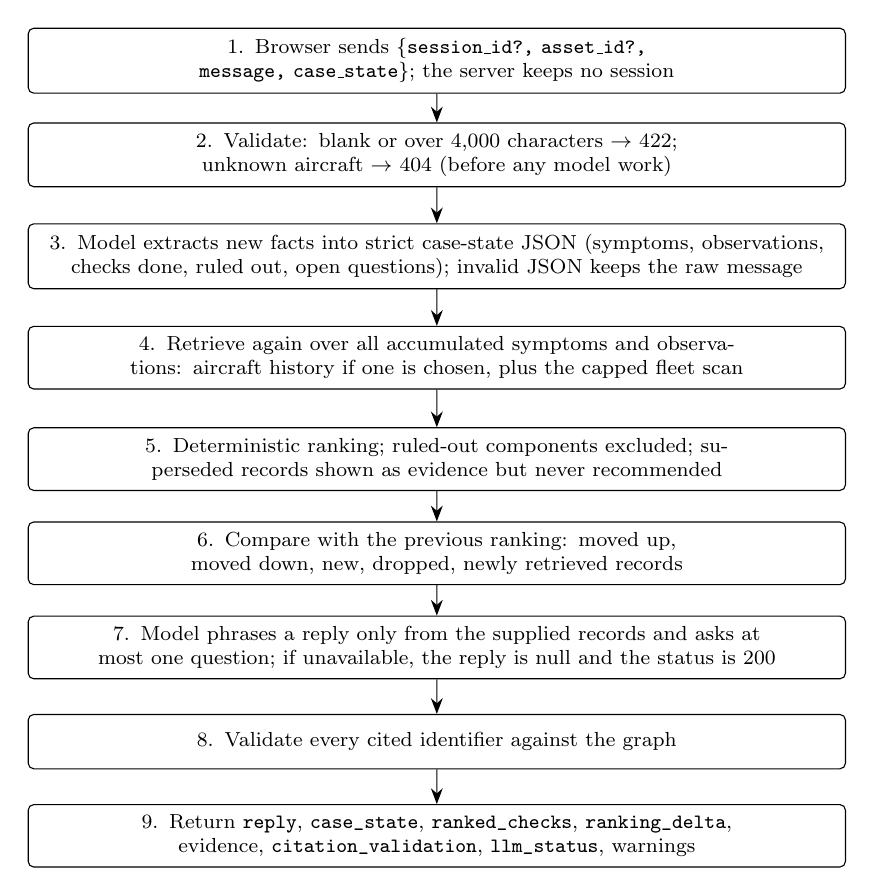
\begin{tikzpicture}[scale=0.92,transform shape,wbox/.style={box,text width=11cm}]
\node[wbox] (a) at (0,0) {1. Browser sends \texttt{\{session\_id?, asset\_id?, message, case\_state\}}; the server keeps no session};
\node[wbox] (b) at (0,-1.3) {2. Validate: blank or over 4,000 characters $\to$ 422; unknown aircraft $\to$ 404 (before any model work)};
\node[wbox] (c) at (0,-2.7) {3. Model extracts new facts into strict case-state JSON (symptoms, observations, checks done, ruled out, open questions); invalid JSON keeps the raw message};
\node[wbox] (d) at (0,-4.1) {4. Retrieve again over all accumulated symptoms and observations: aircraft history if one is chosen, plus the capped fleet scan};
\node[wbox] (e) at (0,-5.5) {5. Deterministic ranking; ruled-out components excluded; superseded records shown as evidence but never recommended};
\node[wbox] (f) at (0,-6.8) {6. Compare with the previous ranking: moved up, moved down, new, dropped, newly retrieved records};
\node[wbox] (g) at (0,-8.1) {7. Model phrases a reply only from the supplied records and asks at most one question; if unavailable, the reply is null and the status is 200};
\node[wbox] (h) at (0,-9.4) {8. Validate every cited identifier against the graph};
\node[wbox] (i) at (0,-10.7) {9. Return \code{reply}, \code{case_state}, \code{ranked_checks}, \code{ranking_delta}, evidence, \code{citation_validation}, \code{llm_status}, warnings};
\foreach \a/\b in {a/b,b/c,c/d,d/e,e/f,f/g,g/h,h/i} {\draw[arr] (\a) -- (\b);}
\end{tikzpicture}

\caption{Processing of one Copilot turn.}\label{fig:copilot}
\end{figure}

\section*{Frontend routes and the data they read}
\begin{longtable}{p{0.36\textwidth}p{0.22\textwidth}p{0.34\textwidth}}
\toprule \textbf{Route} & \textbf{Page} & \textbf{Main endpoint(s)} \\ \midrule \endhead
\code{/app/assets} & Assets & \pth{GET /maintenance/assets} \\
\pth{/app/asset-history/:id} (optionally with \#record) & Asset History & \code{GET /maintenance/assets/{id}/history} \\
\code{/app/records} & Service Records & \pth{GET /maintenance/records}, \code{/assets} \\
\code{/app/diagnostics} & Diagnostics & \pth{POST /maintenance/copilot/turn}, \code{/diagnose} \\
\code{/app/review-queue} & Review Queue, Detected corrections & \code{GET /review-queue}, \code{/corrections}; \code{POST} accept, reject \\
\pth{/app/maintenance-ingest} & Ingest & \pth{POST /maintenance/ingest/upload}, \code{/ingest}, \code{/records} \\
\code{/app/graph} & Knowledge Graph & \code{GET /graph/overview} \\
\code{/app/settings} & Settings and system status & \code{GET /health} \\
\bottomrule
\end{longtable}

\chapter{Meeting and Progress Evidence}\label{app:progress}
\section*{Dated progress documents}
The repository keeps dated evidence documents under \texttt{docs/mid1/}. Table~\ref{tab:progressdocs} lists each with the date it was first committed (from the git history at commit \code{36a98a3}); a later edit does not change the date shown.
\begin{longtable}{p{0.14\textwidth}p{0.36\textwidth}p{0.4\textwidth}}
\caption{Evidence documents with their commit dates}\label{tab:progressdocs}\\
\toprule \textbf{First committed} & \textbf{File} & \textbf{Title} \\ \midrule \endfirsthead
\toprule \textbf{First committed} & \textbf{File} & \textbf{Title} \\ \midrule \endhead
2026-10-16 & \texttt{02\_frontend\_evidence.md} & Frontend evidence --- FYP-I Mid \\
2026-10-15 & \texttt{04\_data\_conflict\_devops\_evidence.md} & Muhammad Usman Al Haq --- Data, Conflict, Testing and DevOps Evidence \\
2026-10-15 & \texttt{05\_usman\_final\_audit.md} & Usman final verification, remediation, and evidence closure \\
2026-10-16 & \texttt{06\_demo\_script.md} & Mid-I demo script and defence notes \\
2026-10-15 & \texttt{06\_frontend\_review\_queue\_handoff.md} & Frontend owner handoff: Review Queue test gate \\
2026-10-15 & \texttt{07\_usman\_release\_readiness.md} & Usman Mid-I release readiness \\
2026-10-16 & \texttt{08\_repository\_hygiene\_and\_handoff.md} & Repository hygiene and release handoff audit \\
2026-10-16 & \texttt{08\_umar\_progress.md} & Umar Mid-I final verification, evidence, and partner closure \\
2026-10-16 & \texttt{09\_frontend\_shared\_api.md} & Frontend $\to$ shared staging API (Mid-I) \\
2026-10-16 & \texttt{10\_perf\_assets\_api\_handoff.md} & Mid-I performance handoff --- slow frontend loads \\
2026-10-16 & \texttt{11\_u2\_real\_data\_retrieval.md} & U2 --- Real-data graph retrieval (staging + Neo4j proof) \\
2026-10-16 & \texttt{12\_u4\_u5\_diagnostics\_handoff.md} & U4 / U5 --- Citation boundary, LLM gate, diagnose tests, UI handoff \\
2026-10-16 & \texttt{13\_u3\_deterministic\_ranking.md} & U3 --- Deterministic ranking and provenance \\
2026-10-16 & \texttt{14\_usman\_umar\_integration.md} & Usman + Umar Mid-I integration audit \\
2026-10-16 & \texttt{15\_report\_mid1\_addendum.md} & Halite FYP-I Mid Report Addendum \\
2026-10-16 & \texttt{16\_backend\_release\_hygiene.md} & Umar + Usman Mid-I backend release hygiene \\
2026-10-16 & \texttt{16\_usman\_conflict\_score\_backfill\_handoff.md} & Usman handoff --- corpus is unscored (all confidence=1 / auto\_accepted) \\
2026-10-17 & \texttt{17\_diagnostic\_copilot\_evidence.md} & Diagnostic copilot evidence --- 2026-10-17 \\
2026-10-17 & \texttt{19\_confidence\_and\_corrections\_evidence.md} & Confidence, fleet records, and corrections evidence --- 2026-10-17 \\
2026-10-17 & \texttt{20\_analysis\_cost\_report.md} & Conflict-analysis cost and quality report --- 2026-10-17 \\
2026-10-17 & \texttt{21\_analysis\_cascade\_evidence.md} & Conflict-analysis cost cascade evidence --- 2026-10-17 \\
2026-10-17 & \texttt{22\_cursor\_handoff\_2026-10-17.md} & Halite FYP --- corrected Cursor handoff \\
2026-10-18 & \texttt{23\_single\_aircraft\_analysis\_evidence.md} & Single-aircraft conflict analysis --- 800NN \\
\bottomrule
\end{longtable}
Document \texttt{24\_live\_revalidation\_2026-10-18.md} (the live re-validation of the diagnosis path, which found and fixed a defect) was added at commit \code{06bc614}, after the snapshot above, and is dated 18 October 2026.

\section*{Supervisor meetings}
No supervisor meeting minutes are stored in the repository, and none are reproduced here. The dated documents above are the progress evidence. Meeting dates and notes can be added if the evaluation asks for them.


\bibliographystyle{plainnat}
\bibliography{references/references}
\end{document}

